\documentclass[a4paper,12pt]{ctexbook}

\usepackage{amsmath}
\usepackage{amssymb}
\usepackage{caption}
\usepackage[colorlinks=true]{hyperref}
\usepackage{graphicx}
\usepackage{float}
\usepackage{tikz}
\usepackage{subfigure}
\usepackage{pgfplots}

\newtheorem{example}{例}[chapter]
\newtheorem{definition}{定义}[chapter]
\newtheorem{theorem}[definition]{定理}
\newtheorem{remark}{注解}
\newtheorem{proof}{证明}
\newtheorem{algorithm}{算法}
\newtheorem{axiom}{公理}
\newtheorem{property}{性质}
\newtheorem{proposition}{命题}
\newtheorem{lemma}{引理}
\newtheorem{corollary}{推论}
\newtheorem{condition}{条件}
\newtheorem{conclusion}{结论}
\newtheorem{assumption}{假设}

% 常用命令的简写
\newcommand{\mb}[1]{\mathbb{#1}}
\newcommand{\mc}[1]{\mathcal{#1}}
\newcommand{\bs}[1]{\boldsymbol{#1}}
\newcommand{\spn}{\mathrm{span}}
% \newcommand{\spn}[1]{\mathrm{span}\left\lbrack #1 \right\rbrack}
\newcommand{\rk}{\mathrm{rk}}
\newcommand{\id}{\mathrm{id}}
\renewcommand{\Im}{\mathrm{Im}}
\newcommand{\innerproduct}[2]{\left\langle#1,#2\right\rangle}
\newcommand{\norm}[1]{\left\|#1\right\|}
\newcommand{\tr}[1]{\mathrm{tr}\left( #1 \right)}
\newcommand{\rad}{\mathrm{rad}}

% 常用符号的简写
\newcommand{\R}{\mathbb{R}}
\newcommand{\A}{\bs{A}}
\newcommand{\B}{\bs{B}}
\newcommand{\T}{\bs{T}}
\newcommand{\I}{\bs{I}}
\newcommand{\D}{\bs{D}}
\newcommand{\U}{\bs{U}}
\newcommand{\V}{\bs{V}}
\renewcommand{\L}{\bs{L}}
\renewcommand{\S}{\bs{S}}
\renewcommand{\P}{\bs{P}}
\newcommand{\x}{\bs{x}}
\newcommand{\y}{\bs{y}}
\newcommand{\z}{\bs{z}}
\newcommand{\e}{\bs{e}}
\newcommand{\g}{\bs{g}}
\renewcommand{\a}{\bs{a}}
\renewcommand{\b}{\bs{b}}
\renewcommand{\c}{\bs{c}}
\renewcommand{\u}{\bs{u}}
\renewcommand{\v}{\bs{v}}
\newcommand{\p}{\bs{p}}
\newcommand{\w}{\bs{w}}
\newcommand{\0}{\bs{0}}

\begin{document}

\author{翻译 by NothNess , 感谢原书作者}
\title{机器学习中的数学}
\date{从2021年07月18日 -- 今 }

\frontmatter
\maketitle
\tableofcontents
\chapter{前言}

机器学习是一种最新的尝试,它试图将人类的知识和逻辑提炼成适合构建机器和工程自动化的系统.
随着机器学习变得越来越普遍,它的软件包也变得越来越易于使用,
很自然的,也是人们所希望的, 一些底层的技术细节被抽象出来, 学习者(practitioner)无从得知.
然而, 这带来了一些危险,即学习者并不了解相关设计的原因,因此也不知道机器学习算法的局限性.

那些有兴趣了解机器学习算法背后魔力的热情学习者面临着一些令人生畏的先决知识:

\begin{itemize}
	\item 编程语言和数据分析工具
	\item 大规模计算和相关框架
	\item 数学, 统计学, 以及机器学习是如何在此基础上构建的
\end{itemize}

在大学里,关于机器学习的入门课程通常在课程的早期就会涉及到这些知识. 
由于历史原因,机器学习课程往往在计算机科学系被教授,学生通常在前两个知识领域接受训练,但在数学和统计学方面则没有那么多.

当前的机器学习教科书主要侧重于机器学习算法和方法,并假设读者擅长数学和统计学. 
因此,这些书只在书的开头或附录中用了一两章介绍相关数学知识. 
我们发现很多人本来想要深入研究机器学习的理论知识,结果却在为弄明白其中的数学知识而苦苦挣扎. 
在大学教授本科和研究生课程后,我们发现高中数学与阅读标准机器学习教科书所需的数学水平之间的差距对很多人来说太大了.

本书将基本机器学习概念的数学基础放在首位,并将所有信息集中在一起,从而缩小甚至完全弥补了这种技能差距.

\begin{center}
	\textbf{为什么又是一本关于机器学习的书?}
\end{center}

机器学习建立在数学语言的基础上,用以表达看似直观但难以形式化的概念. 
一旦正确形式化,我们就可以深入了解我们想要解决的任务.
全球数学专业学生的一个普遍抱怨是:所学习的主题似乎与实际问题几乎没有关系.
我们相信机器学习是人们学习数学的明显而直接的动机.

\marginpar{数学在大众心目中与恐惧和焦虑相联系. 你会认为我们是在讨论蜘蛛. (Strogatz, 2014, page 281)}
这本书的目的是作为众多数学文献的指南, 成为现代机器学习的基石.
我们通过直接指出数学概念在基本机器学习问题的背景下的有用性来激起学习数学概念的需求.
为了使这本书保持简短,许多细节和更先进的概念被省略了.
在了解了这里提出的基本概念,以及它们如何适应机器学习的更大背景之后,读者可以找到大量的资源进行进一步的研究,我们将在相关章节的末尾提供这些资源.
对于具有数学背景的读者,本书简要但准确地介绍了机器学习.
与其他专注于机器学习方法和模型的书籍相比
(MacKay,2003;Bishop,2006;Alpaydin,2010;Barber,2012;Murphy,2012;Shalev-Shwartz 和 Ben-David,2014;Rogers 和 Girolami,2016)
或机器学习的程序方面
(Müller Guido,2016;Raschka 和 Mirjalili,2017;Chollet 和 Allaire,2018),
我们只提供了机器学习算法的四个代表性示例.同时,我们专注于模型本身背后的数学概念.我们希望读者能够对机器学习中的基本问题有更深入的理解,并将机器学习中出现的实际问题与数学模型选择联系起来.

我们的目标不是写一本经典的机器学习书籍. 相反,我们的目的是提供应用于四个核心机器学习问题的数学基础,以便更容易阅读其他机器学习教科书.

\begin{center}
	\textbf{谁适合看本书?}
\end{center}

随着机器学习在社会中的应用越来越广泛,我们相信每个人都应该对其基本原理有所了解. 本书以学术数学风格编写,使我们能够准确了解机器学习背后的概念. 
我们鼓励不熟悉这种看似简洁的风格的读者坚持不懈,并牢记每个主题的目标.
我们在整篇文章中有大量的评论和注释,希望它为您的整体理解提供有用的指导.

本书假设读者具有高中数学和物理中常见的数学知识. 
例如,读者之前应该已经看过微分和积分,以及二维或三维的几何向量.
从这里开始,我们归纳这些概念. 因此,本书的目标读者包括本科大学生、自学者和参加在线机器学习课程的学习者.

与音乐类似,人们与机器学习有三种类型的交互:

\paragraph{精明的倾听者} 通过提供开源软件、在线教程和基于云的工具,机器学习的大众化使用户不必担心这些过程的细节. 用户可以专注于使用现成的工具从数据中提取见解. 这使得不精通技术的领域专家能够从机器学习中受益,这类似于听音乐; 用户能够选择和辨别不同类型的机器学习,并从中受益. 更有经验的用户就像音乐评论家一样,询问有关机器学习在社会中应用的重要问题,例如道德、公平和个人隐私. 我们希望本书为思考机器学习系统的认证和风险管理提供了基础,并允许他们利用他们的领域专业知识来构建更好的机器学习系统.

\paragraph{经验丰富的艺术家} 熟练的机器学习从业者可以将不同的工具和库插入到分析过程中. 典型的从业者是数据科学家或工程师,他们了解机器学习接口及其用例,并且能够从数据中进行出色的预测. 这类似于演奏音乐的演奏家,高技能的从业者可以将现有的乐器带入生活,并为观众带来乐趣. 使用此处介绍的数学作为入门,从业者将能够了解他们最喜欢的方法的优点和局限性,并扩展和概括现有的机器学习算法. 我们希望本书为机器学习方法的更严格和更有原则的发展提供动力.

\paragraph{初出茅庐的作曲家} 随着机器学习应用于新领域,机器学习开发人员需要开发新方法并扩展现有算法. 这些研究人员需要了解机器学习的数学基础并发现不同任务之间关系. 这类似于音乐作曲家,他们在音乐理论的规则和结构内,创作出令人惊叹的新作品.我们希望这本书为那些想成为机器学习作曲家的人提供其他技术书籍的高水平概述.社会需要新的研究人员,他们能够提出和探索新的方法来应对数据学习中的更多挑战.

\begin{center}
	\textbf{致谢}
\end{center}

我们感谢许多看过本书早期草稿并经历了痛苦的概念阐述的人. 不是原则性的问题,我们尽量试图实现他们的想法.
我们要特别感谢 Christfried Webers 对本书许多部分的仔细阅读,以及他对结构和表述的详细建议. 
许多朋友和同事也很友好地为每一章的不同版本付出了他们的时间和精力. 
我们很幸运地受益于在线社区的慷慨解囊,他们通过 https://github.com 提出了改进建议,这极大地改进了本书. 
以下人员通过 https://github.com 或个人交流发现了错误、建议的澄清和建议的相关文献. 他们的名字按字母顺序排列.

Abdul-Ganiy Usman

Adam Gaier

Adele Jackson

Aditya Menon

Alasdair Tran

Aleksandar Krnjaic

Alexander Makrigiorgos

Alfredo Canziani

Ali Shafti

Amr Khalifa

Andrew Tanggara

Angus Gruen

Antal A. Buss

Antoine Toisoul Le Cann

Areg Sarvazyan

Artem Artemev

Artyom Stepanov

Bill Kromydas

Bob Williamson

Boon Ping Lim

Chao Qu

Cheng Li

Chris Sherlock

Christopher Gray

Daniel McNamara

Daniel Wood

Darren Siegel

David Johnston

Dawei Chen

Ellen Broad

Fengkuangtian Zhu

Fiona Condon

Georgios Theodorou

He Xin

Irene Raissa Kameni

Jakub Nabaglo

James Hensman

Jamie Liu

Jean Kaddour

Jean-Paul Ebejer

Jerry Qiang

Jitesh Sindhare

John Lloyd

Jonas Ngnawe

Jon Martin

Justin Hsi

Kai Arulkumaran

Kamil Dreczkowski

Lily Wang

Lionel Tondji Ngoupeyou

Lydia Kn¨ufing

Mahmoud Aslan

Mark Hartenstein

Mark van der Wilk

Markus Hegland

Martin Hewing

Matthew Alger

Matthew Lee

Maximus McCann

Mengyan Zhang

Michael Bennett

Michael Pedersen

Minjeong Shin

Mohammad Malekzadeh

Naveen Kumar

Nico Montali

Oscar Armas

Patrick Henriksen

Patrick Wieschollek

Pattarawat Chormai

Paul Kelly

Petros Christodoulou

Piotr Januszewski

Pranav Subramani

Quyu Kong

Ragib Zaman

Rui Zhang

Ryan-Rhys Griffiths

Salomon Kabongo

Samuel Ogunmola

Sandeep Mavadia

Sarvesh Nikumbh

Sebastian Raschka

Senanayak Sesh Kumar Karri

Seung-Heon Baek

Shahbaz Chaudhary

Shakir Mohamed

Shawn Berry

Sheikh Abdul Raheem Ali

Sheng Xue

Sridhar Thiagarajan

Syed Nouman Hasany

Szymon Brych

Thomas B¨uhler

Timur Sharapov

Tom Melamed

Vincent Adam

Vincent Dutordoir

Vu Minh

Wasim Aftab

Wen Zhi

Wojciech Stokowiec

Xiaonan Chong

Xiaowei Zhang

Yazhou Hao

Yicheng Luo

Young Lee

Yu Lu

Yun Cheng

Yuxiao Huang

Zac Cranko

Zijian Cao

Zoe Nolan

通过 GitHub 的贡献者(其真实姓名未在其 GitHub 个人资料中列出)是:

SamDataMad

bumptiousmonkey

idoamihai

deepakiim

insad

HorizonP

cs-maillist

kudo23

empet

victorBigand

17SKYE

jessjing1995

我们也非常感谢 Parameswaran Raman 和剑桥大学出版社组织的许多匿名审稿人,他们阅读了手稿早期版本的一章或多章,并提出了建设性的批评意见,从而带来了相当大的改进. 特别值得一提的是 Dinesh Singh Negi,我们的 LATEX 支持人员,提供有关 LATEX 相关问题的详细而及时的建议. 最后但同样重要的是,我们非常感谢我们的编辑 Lauren Cowles,他一直耐心地指导我们完成本书的构思过程.
\renewcommand\arraystretch{0.8}
\begin{table}
\caption*{\textbf{Table of Symbols}}
\begin{tabular}{llp{\textwidth}}
    \hline
    Symbol & Typical meaning \\
    \hline
    \hline
    $a, b, c, \alpha, \beta, \gamma$ & 标量是小写字母 \\
    $\x, \y, \bs{z}$ & 向量是加粗小写字母 \\
    $\A, \B, \bs{C}$ & 矩阵是加粗大写字母 \\
    $\x^\top, \A^\top$  & 向量或矩阵的转置 \\
    $\A^{-1}$ & 逆矩阵 \\
    $\langle \x, \y \rangle$ & $\x$ 和$\y$ 的内积 \\
    $\x \cdot \y$ & $\x$ 和$\y$ 的点积 \\
    $B=(\b_1, \b_2, \b_3)$ & (有序) 元组 \\
    $\B=[\b_1, \b_2, \b_3]$ & 列向量水平堆叠构成矩阵 \\
    $\mc{B} = \{\b_1, \b_2, \b_3 \}$ & 向量的集合(无序) \\
    $\mb{Z}, \mb{N}$ & 整数和自然数 \\
    $\R, \mb{C}$ & 实数和负数 \\
    $\R^n$ & 实数域n维向量空间(vector space) \\
    \hline
    $\forall x$ & 全称量词:对于所有$x$ \\
    $\exists x$ & 存在量词: 至少存在一个$x$ \\
    $a:=b$ & a 被定义为b \\
    $a=:b$ & b 被定义为a \\
    $a \propto b$ & a 与 b成 正比例,i.e.,$a = constant \cdot b$\\
    $g \circ f$ & 函数复合:"f 后是 g" \\
    $\Longleftrightarrow$ & 当且仅当 \\
    $\Longrightarrow$ & 蕴涵 \\
    $\mc{A}, \mc{C}$ & 集合 \\
    $a \in \mc{A}$ & $a$ 是集合$\mc{A}$的一个元素 \\
    $\emptyset$ & 空集 \\
    $\mc{A} \backslash \mc{B}$ & 排除$\mc{B}$的$\mc{A}$:
            所有在$\mc{A}$ 但是不在 $\mc{B}$中的元素的集合 \\
    $D$ & 维数, $d = 1, ... D$ \\
    $N$ & 数据点(data points)的个数, $n = 1,..., N$ \\
    \hline
    $\bs{I}_m$ & 大小为$m \times m$的矩阵 \\
    $\bs{0}_{m,n}$ & 大小为$m \times n$的0矩阵 \\
    $\bs{1}_{m,n}$ & 大小为$m \times n$的1矩阵 \\
    $\e_i$ & 标准/规范向量 \\
    $\dim$ & 向量空间的维 \\
    $\rk(\A)$ & 矩阵$\A$的秩(rank) \\
    $\Im(\Phi)$ & 线性映射$\Phi$的像(image) \\
    $\ker(\Phi)$ & 线性映射$\Phi$ 核(null space, 零空间) \\
    $\spn[\b_1]$ & $\b_1$ 的 张成空间(Span, gererating set) \\
    $\mathrm{tr}(\A)$ & $\A$的迹(trace) \\
    $\det(\A)$ & $\A$的行列式(determinant) \\
    $|\cdot|$ & 行列式的绝对值(取决于上下文) \\
    $\| \cdot \|$ & 范数(norm);未特别指出则均指代欧几里德范数 \\
    $\lambda$ & 特征值(eigenvalue)/拉格朗日乘数(Lagrange multiplier) \\
    $E_\lambda$ & 特征值$\lambda$对应的特征空间(eigenspace) \\
    \hline
\end{tabular}
\end{table}

\begin{table}
\begin{tabular}{llp{\textwidth}}
	\hline
	Symbol & Typical meaning \\
	\hline
	\hline
	$ \x \perp \y $ & 向量$\x$和向量$\y$正交 \\
	$V$ & 向量空间 \\
	$V^\top$ & 向量空间$V$的正交补(orthogonal complement) \\
	$\sum_{n=1}^{N}x_n$ & Sum of the $x_n: x_1 + ... + x_N$ \\
	$\prod_{n=1}^{N}x_n$ & Product of the $x_n: x_1 \cdot ... \cdot x_N$ \\
	$\bs{\theta}$ & 参数向量 \\
	$ \frac{\partial f}{\partial x} $ & $f$关于$x$的偏导数 \\
	$ \frac{\mathrm{d} f}{\mathrm{d} x} $ & $f$关于$x$的导数 \\
	$ \nabla $ & 梯度{gradient} \\
	$ f_* = \min_x f(x) $ & 函数$f$的最小函数值 \\
	$ x_* \in \arg \min_x f(x) $ & $x_*$使$f$最小化(注意:$\arg \min$返回一组值) \\
	$ \mathfrak{L}$ & 拉格朗日(Lagrangian) \\
	$ \mc{L}$ & 负对数似然(negative log-likelihood) \\
	$\binom{n}{k}$ & 二项式系数, n个选k个\\
	$\mb{V}_X[\x]$ & $\x$相对于随机变量$X$ 的方差 \\
	$\mb{E}_X[\x]$ & $\x$相对于随机变量$X$ 的期望 \\
	$\mathrm{Cov}_{x,y}[\x, \y]$ & $x,y$的协方差 \\
	$X \perp \!\!\! \perp Y | Z$ & 给定$Z$, $X$条件独立于$Y$ \\
	$\mc{N}(\bs{\mu}, \bs{\Sigma})$ & 随机变量 $X$ 依据 $p$ 分布 \\
	$\mathrm{Ber}(\mu)$ & 参数为$\mu$的伯努利分布(Bernoulli distribution) \\
	$\mathrm{Bin}(N, \mu)$ & 参数为$N, \mu$的二项分布(Binomial distribution) \\
	$\mathrm{Beta}(\alpha, \beta)$ & 参数为$N, \mu$的Beta分布 \\
	\hline
\end{tabular}
\end{table}

\begin{table}
\caption*{\textbf{Table of Abbreviations and Acronyms}}
\begin{tabular}{llp{\textwidth}}
	\hline
	Acronym(首字母缩略词) & Meaning \\
	\hline
	\hline
	e.g. & 例如 \\
	GMM & 高斯混合模型(Gaussian mixture model) \\
	i.e & 这意味着,意思是。.(this means)\\
	i.i.d & 独立, 等同分布(independent, identically distributed) \\
	MAP & 最大后验(maximum a posteriori) \\
	MLE & 最大似然估计(maximum likelihood estimation/estimator) \\
	ONB & 正交基(orthonormal basis) \\
	PCA & 主成分分析(Principal component analysis) \\
	PPCA & 概率主成分分析(Probabilistic PCA) \\
	REF & 行阶梯形矩阵(Row-echelon form) \\
	SPD & 对称正定(Symmetric, positive definite) \\
	SVM & 支持向量机(Support vector machine) \\
	\hline
\end{tabular}
\end{table}



\mainmatter

\part{数学基础}
\chapter{简介和起因}
机器学习和设计从数据中自动提取有价值信息的算法息息相关。
这里的重点在于"自动",
i.e., 当处理有意义的事物时, 机器学习关注可以用于多个数据集(dataset)的通用方法论(general-purpose methodologies).
机器学习有三个核心概念: 数据, 模型, 学习(data, a model, and learning).

\marginpar{数据}
因为机器学习本身就是数据驱动的, 数据是机器学习的核心。
机器学习的目的就是设计通用方法来从数据中提取有价值的模式(patterns), 理想情况下不需要太多领域特定知识。
例如, 给定一个大型文档语料库(e.g., 许多图书馆的书), 机器学习方法能够自动查找相关主题, 这些主题是跨文档共享的(Hoffman et al., 2010).
\marginpar{模型}
为了实现这个目的, 我们设计通常和生成数据过程相关的模型, 和我们给定的数据集类似。
例如, 在回归中, 模型描述一个函数, 该函数映射输入到一个实值输出。
转述Mitchell(1997): 如果在考虑数据后模型在给定任务上的性能有所提高,则称该模型从数据中学习。
目的是找到能够很好的概括未知数据(即, 泛化能力强)的好模型, 这我们以后或许会关心。
\marginpar{学习}
学习可以理解为一种通过优化模型参数自动寻找数据中模式和结构的方式。

机器学习已经有过许多成功案例, 设计和训练复杂而灵活的机器学习系统的软件一应俱全。
我们相信这本机器学习数学基础对于理解基础原则是十分重要的, 更复杂的机器学习系统都构建在这些基础原则上。
理解这些原则能够促进创建新的机器学习解决方案, 理解和调试已经存在的方法, 和学习方法学固有的假设和局限

\section{凭直觉理解单词}
在机器学习中我们经常遇到的一个挑战就是那些概念和单词都十分棘手,
并且一个机器学习系统的特定部分会被抽象为不同的数学概念。
例如, 单词"算法(algorithm)"在机器学习语境中至少有两个不同的应用场景。
第一个场景中, 我们用短语"机器学习算法"代表一个根据输入数据做出预测的系统。
我们称这些算法为预测器(predictors).\marginpar{预测器}
第二个场景中, 我们用相同的短语"机器学习算法"代表一个适应预测器内部参数的系统, 这样它在处理未知输入数据时能表现良好。
我们称这种适应为"训练"一个系统。\marginpar{训练}

这本书不会解决歧义问题, 但我们希望预先强调这些: 取决于上下文, 相同的表述可能意味着不同的事物。
虽然如此, 我们将尝试给出一个清晰的上下文以减少歧义。

这本书的第一部分介绍了关于机器学习三大概念:数据,模型, 学习需要知道的数学概念和数学基础。
我们在这里简要的列出大纲, 当我们讨论必须的数学概念时, 我们会再看到他们。

因为并非所有数据都是以数字表示的, 将数据视作数字格式常常有用。
本书中, 我们假设数据已经被恰当的转换为数字表示并且适合被计算机程序读取。
所以, 我们可以将数据视为向量 \marginpar{将数据视作向量}.
作为另一个说明词是多么微妙的例子, (至少)有三种不同的方式来思考向量:
向量是一个数字数组(计算机科学视角),
向量是一个有大小和方向的箭头(物理视角),
向量是一个服从加法(addition)和乘法(scaling)的对象(数学视角)。

一个模型\marginpar{模型}经常被用来描述生成数据的过程, 类似于手头的数据集。
因此, 好的模型会被视作简化版本的真实(未知)数据生成过程, 从中获取数据建模和提取隐藏模式相关的方面。
一个好的模型没有在真实世界实验就可以很好的预测真实世界会发生什么。

现在我们到了问题的关键--机器学习中的学习\marginpar{学习}.
假设我们给定了一个数据集和合适的模型。
训练这个模型意味着使用可获取的数据依据效用函数(utility functioin)优化模型的一些参数,
效用函数估计出模型预测训练数据有多好。
多数训练方法可以看作是一种爬山登顶的方法。
在这个比喻中, 峰顶对应着一些你希望的性能指标的最大化。
然而, 在实践中, 我们对模型处理未知数据表现良好的模型很感兴趣。
在处理我们已知的数据(训练数据)中表现良好, 可能仅仅意味着我们找到了一个很好的方法来记忆数据。
但是, 这不能很好的泛化到未知数据, 并且不能实际应用, 我们经常需要机器学习系统处于他从未遇到过的环境中。

让我们总结一下我们在本书中介绍的机器学习中的重要概念:

\begin{itemize}
	\item 我们将数据视作向量
	\item 我们选择恰当的模型, 无论从概率视角或优化视角
	\item 我们从可获取的数据中使用数学优化方法学习, 目的是在接受非训练数据时也能表现良好
\end{itemize}

\section{阅读本书的两种方式}

我们有两种策略来理解机器学习中的数学:

\begin{itemize}
	\item \textbf{自底向上:}
	从基础开始到高级逐渐构建概念。 这在学习技术领域是最好的方法, 例如数学。
	这种策略的优点是读者可以在任意时刻回顾先前学习的概念。
	不幸的是, 对于学习者, 许多基础概念对他们来说并不十分有趣, 而缺少动机意味着大量的基本定义会很快遗忘。
	\item \textbf{自顶向下:}
	从实践中钻研需要更多基础需求。
	这类目标驱动方式有着自己的优点:在任何时刻,读者都知道为什么他们需要研究某一概念, 并且明确获取所需知识的途径。
	这种策略的缺点是知识可能构建在不稳定的基础之上, 读者需要记忆一系列他们没有办法理解单词。
\end{itemize}

我们决定以模块化的方式写这本书, 这样分开(数学的)基础概念, 读者就可以以上面两种方式阅读本书了。
这本书分为两部分, 第一部分奠定数学基础, 第二部分应用从第一部分学到的概念解决一些基础的机器学习问题,
这些问题形成机器学习的四大支柱(参见 图1.1):
回归(regression), 降维(demensionality), 密度估计(density estimation), 和分类(classification).
第一部分的章节多数都构建在前一章之上, 但是跳过某一章并在需要时跳回阅读是可能的。
第二部分的章节都是松耦合的(loosely coupled)所以可以以任何顺序阅读。
在两部分间有许多向前向后的提示以将数学概念和机器学习算法联系起来。

\begin{figure}
	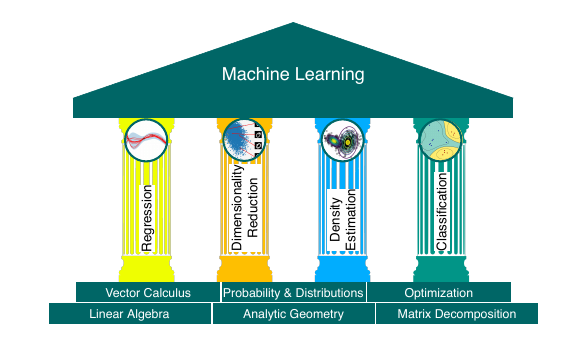
\includegraphics[width=\textwidth]{./chapter01/pillar.png}
	\caption{基石和机器学习四大支柱}
\end{figure}

当然有更多其他方式阅读这本书。
多数读者学习时采用自底向上和自顶向下结合的方式,
有时在尝试复杂概念时先学习基础的数学技巧,
也选择基于机器学习应用的主题进行学习。

\begin{center} 第一部分关于数学 \end{center}
我们在本书中要学习机器学习的四大支柱需要有坚实的数学基础, 这些分布在第一部分中。

我们将数值数据(numerical data)表示为向量, 将这样的数据的表格表示为矩阵。
研究向量和矩阵的就是线性代数, 我们将在第二章介绍。\marginpar{线性代数}
作为向量集合的矩阵也在这里讲述。

给定两个向量来表示真实世界的两个对象, 我们想要对它们的相似性发表看法。
这个想法是:相似的向量通过我们的机器学习算法(预测器)应当能被预测到有相似的输出。
为了形式化这个两向量间相似性的想法, 我们需要介绍一种运算,将两个向量作为输入, 返回一个数值来表示他们的相似性的。
相似的构造和距离是解析几何的重心, 这将在第三章讨论。\marginpar{解析几何}

在第四章, 我们会介绍一些关于矩阵和矩阵分解的基础概念。
一些矩阵运算在机器学习中极其有用, 也允许对数据和更有效的学习进行直觉上的解释。\marginpar{矩阵分解}

我们经常认为数据是对潜在的真实信号的有噪音的观察。
我们希望通过应用机器学习我们可以从噪音中识别信号。
这要求我们有一门语言来量化"噪音"到底是什么。
我们也经常喜欢用允许我们表达某种程度不确定性的预测器来量化我们在特定测试数据点上关于预测值的置信度。
量化不确定性是概率论的领域, 这会在第六章覆盖。\marginpar{概率论}

为了训练机器学习模型, 我们通常寻找使得性能测量最大化的参数。
许多优化技巧需要梯度的概念, 它告诉我们搜索解决方案的方向。
第五章关于向量积分(vector calculus)\marginpar{向量积分}, 并且详细讲述梯度的概念, 随后我们在讨论优化\marginpar{优化}和寻找函数最大/最小值的第七章就要用到。

\begin{center}
	第二部分关于机器学习
\end{center}
本书的第二部分介绍机器学习的四大支柱(正如图1.1所示).
我们会阐明在第一章中学到的数学概念是怎样成为每根支柱的基石的。
宽泛的说, 章节是按照难度升序排列的。

在第 8 章中,我们以数学方式重申机器学习的三个组成部分(数据、模型和参数估计(parameter estimation)).
在此外,我们提供了一些构建实验配置的指南, 防止对机器学习系统过于乐观的估计。
回想一下, 我们的目标是构建一个在未知数据上表现良好的预测器。

在第 9 章中,我们将仔细研究线性回归\marginpar{线性回归},
其中我们的目标是找到将输入 $\x \in \R^D$ 映射到对应的观测函数值 $y \in \R$,
我们可以将其解释为它们各自输入的标签。
我们将通过最大似然和最大后验估计以及贝叶斯线性回归讨论经典模型拟合(参数估计), 我们整合参数而不是优化它们。

\marginpar{降维}
第 10 章重点介绍降维,即图 1.1 中的使用主成分分析的第二个支柱。
降维的关键目标是找到高维数据 $\x \in \R^D$ 的紧凑、低维表示,这通常比原始数据更容易分析。
与回归不同,降维只关心数据建模 -- 没有与数据点 $\x$ 相关联的标签。

\marginpar{密度估计}
在第 11 章中,我们将转到第三个支柱:密度估计。
密度估计的目标是找到描述给定数据集的概率分布。
为此, 我们将专注于高斯混合模型, 我们将讨论一个迭代方案来找到这个模型的参数。
与降维一样,没有与数据点 $\x \in \R^D$ 相关联的标签。
但是,我们不寻求数据的低维表示。
相反,我们对描述数据的密度模型感兴趣。

\marginpar{分类}
本书12章进一步讨论了第四根支柱: 分类。
我们将在支持向量机的背景下讨论分类。
类似于回归(第 9 章),我们有输入 $\x$ 和相应的标签 $y$.
然而,与回归不同,其中标签是实值的,分类中的标签是整数,这需要特别注意。

\section{练习题和反馈}

我们在第一部分提供了一些练习, 多数可以用纸笔完成。
对于第二部分,我们提供了编程教程(jupyter notebooks)来探索我们在本书中讨论的机器学习算法的一些特性。
我们感谢剑桥大学出版社大力支持我们旨在通过免费制作本书来实现教育和学习的民主化, 可在
\begin{center}
	\url{https://mml-book.com}
\end{center}
下载,可以在其中找到教程、勘误表和其他材料。
可以使用上述 URL 报告错误并提供反馈。

\chapter{线性代数}
在形式化直觉概念时,一种常见的方法是构造一组对象(符号)和一组操作这些对象的规则。
这被称为代数。\marginpar{代数}
线性代数研究向量和操纵向量的规则。
我们很多人在学校知道的向量被称为“几何向量”,通常用字母上方的小箭头表示,例如
$\vec{x} , \vec{y}$
在本书中,我们讨论更一般的
向量的概念并使用粗体字母来表示它们,例如 $\x$ 和 $\y$。

通常,向量是特殊的对象,可以将它们相加和乘以标量以产生另一个相同类型的对象。
从抽象的数学角度来看,任何满足这两个属性的对象都可以被认为是一个向量。
以下是此类向量对象的一些示例:

\begin{enumerate}
    \item 几何向量。
    这个向量的例子在学校数学和物理课上可能已经很熟悉了。
    几何向量——见图 2.1(a) – 是有向线段,可以绘制(至少在两个维度上).
    两个几何向量 $\vec{\x}$ 和 $\vec{\y}$可以相加,
    使得 $\vec{\x} + \vec{\y} = \vec{\bs{z}}$
    是另一个几何向量。
    此外,乘以标量$\lambda \vec{\x}, \lambda \in \R$, 也是一个几何向量。
    这其实就是将原始向量缩放$\lambda$倍。
    因此,几何向量是之前介绍的向量的实例
    将向量解释为几何向量, 使我们能够使用我们对方向和大小的直觉来推理数学运算。

    \item 多项式(polynomials)也是向量;
    见图2.1(b):
    两个多项式也能相加, 结果是另一个多项式;
    也能乘以一个标量$\lambda \in \R$, 结果也是一个多项式。
    因此, 多项式是(尽管不寻常)向量的一个实例。
    注意多项式和几何向量非常不同。
    几何向量能够具体画出, 但是多项式是抽象的概念。
    尽管如此, 他们都是前面提到的向量。

    \begin{figure}
    \subfigure[几何向量]{
    \begin{tikzpicture}
        \draw[thick,-latex] (0,0) -- (0,2) node[left]{$\vec{\x}$};
        \draw[thick,-latex] (0,0) -- (2,4) node[left]{$\vec{\x}+ \vec{\y}$};
        \draw[thick,-latex] (0,0) -- (2,2) node[below]{$\vec{\y}$};
    \end{tikzpicture}
    }
    \subfigure[多项式]{
    \begin{tikzpicture}
        \begin{axis}[xlabel=$x$, ylabel=$y$, domain=-2.5:2.5]
        \addplot[color=red]{-2 * x ^ 2};
        \addplot[color=blue] {-3*x + 3};
        \addplot[color=orange] {(x-2) ^ 2 - 5};
        \end{axis}
    \end{tikzpicture}
    }
    \caption{不同类型的向量。 向量令人惊讶, 包括(a)几何向量和(b)多项式}
    \end{figure}

    \item 音频信号(audio signals)是向量。
    音频信号表示为一系列数字。
    我们可以将两个音频信号相加, 和是一个新的音频信号。
    如果我们缩放(scale)音频信号, 我们也获取一段音频信号。
    因此, 音频信号也是一种向量。

    \item $\R^n$(n个实数的元组) 的元素是向量。
    $\R^n$ 比多项式更抽象, 也是这本书我们关注的重点。 例如:
    \begin{equation}
        \a =
        \begin{bmatrix}
            1 \\ 2 \\ 3
        \end{bmatrix}
        \in \R^3
    \end{equation}
    是一个数字三元组的例子。
    两个向量$\a , \b \in \R^n$ 相加,
    结果是另一个向量$\a + \b = \bs{c} \in \R^n$。
    更进一步, 用$\lambda \in \R$ 乘以 $\a \in \R^n$,
    结果是一个缩放的向量 $\lambda \a \in \R^n$。
    \marginpar{在计算机上实现时, 一定要注意检查数组操作是否真的是一个向量运算}
    将向量看作$\R^n$的元素有额外的好处, 他们松散对应着计算机上的实数数组
    许多编程语言支持数组操作,允许涉及向量运算的算法的便捷实现。
\end{enumerate}

线性代数关注向量概念间的相似性
线性代数侧重于这些向量概念之间的相似性。
我们可以将它们加在一起并乘以标量。
我们将在很大程度上关注 $\R^n$ 中的向量,因为线性代数中的大多数算法都在 $\R^n$ 中制定。
我们将在第 8 章中看到,我们经常将数据视为表示为 $\R^n$ 中的向量。
在本书中,我们将重点关注有限维向量空间,这种情况下在任何类型的向量和 $\R^n$ 之间存在 1:1 的对应关系。
方便的时候我们会用关于几何向量的直觉并考虑基于数组的算法。

数学中的一个主要思想是“闭包”的思想。
这是问题:我提议的操作可能产生的所有事物的集合是什么?
在向量的情况下:从一小组向量开始,然后将它们相加并缩放它们可以得到的向量集是什么?
结果就是向量空间(第 2.4 节)。
向量空间的概念及其属性是机器学习中非常底层的东西。
本章介绍的概念总结在图 2.2 中。

本章主要基于 Drumm和 Weil (2001)、Strang (2003)、Hogben (2013)、Liesen 和 Mehrmann (2015) 的讲义和书籍,以及 Pavel Grinfeld 的线性代数系列。
其他精彩的资源: MIT Gilbert Strang的线性代数课程和3BlueBrown的线性代数系列
\marginpar{
    \tiny{
    Pavel Grinfeld的系列线性代数课: \url{http://tinyurl.com/nahclwm}\\
    Gilber Strang's线性代数课: \url{http://tinyurl.com/29p5q8j}\\
    3BlueBrown线性代数系列课: \url{https://tinyurl.com/h5g4kps}
    }
}

\begin{figure}
    \begin{tikzpicture}[scale=0.4, align=center,rounded corners]
        \fontsize{8}{3}
        \node[fill=blue!20](Vector) at (0,0) {向量};
        \node[fill=blue!20](Matrix) at (-5,-5) {矩阵};
        \node[fill=blue!20](Vector space) at (0, -6) {向量空间};
        \node[fill=blue!20](Group) at (10, -6) {群};
        \node[fill=blue!20](Linear independence) at (17, -6) {线性\\无关};
        \node[fill=blue!20](Basis) at (17, -13) {基};
        \node[fill=blue!20](System of linear equations) at (-12, -10) {线性\\方程组};
        \node[fill=blue!20](Gaussian elimination) at (-12, -17) {高斯\\消元法};
        \node[fill=blue!20](Matrix inverse) at ( -5, -16) {逆矩阵};
        \node[fill=blue!20](Linear/affine mapping) at ( -2, -12) {线性/仿射映射};

        \node[fill=green!20](Chapter3) at (-2, -20) {Chapter3\\解析几何};
        \node[fill=green!20](Chapter5) at (-15, -5) {Chapter5\\向量积分};
        \node[fill=green!20](Chapter10) at (17, -20) {Chapter10\\降维};
        \node[fill=green!20](Chapter12) at (10, -20) {Chapter12\\分类};

        \draw[-latex] (Vector) -- node[above left]{组合} (Matrix);
        \draw[-latex] (Matrix) -- node[above left]{表示} (System of linear equations);
        \draw[-latex] (Matrix) -- node[above left]{表示} (Linear/affine mapping);
        \draw[-latex] (Matrix) --  (Chapter5);
        \draw[-latex] (System of linear equations) -- node[above left]{被解决}(Gaussian elimination);
        \draw[-latex] (System of linear equations) -- node[above right]{解决} (Matrix inverse);

        \draw[-latex] (Vector) -- node[above right]{闭包} (Vector space);
        \draw[-latex] (Vector space) -- (Linear/affine mapping);
        \draw[-latex] (Linear/affine mapping) -- (Chapter3);
        \draw[-latex] (Linear/affine mapping) -- (Chapter12);

        \draw[-latex] (Group) -- node[above]{阿贝尔\\with +} (Vector space);

        \draw[-latex] (Vector) -- node[above right]{的属性}(Linear independence);
        \draw[-latex] (Linear independence) -- node[above right]{最大集} (Basis);
        \draw[-latex] (Basis) -- (Chapter10);
        \draw[-latex] (Basis) -- (Chapter12);
    \end{tikzpicture}
    \caption{本章概念的思维导图, 以及本书其他部分使用它们的地}
\end{figure}

线性代数在机器学习和通用数学中扮演着重要的角色。
本章介绍的概念进一步扩展到第 3 章中的几何概念。
在第 5 章中,我们将讨论向量微积分,其中矩阵运算的基本知识是必不可少的。
在第 10 章中,我们将使用投影(将在第 3.8 节中介绍)通过主成分分析(PCA)进行降维。
在第 9 章中,我们将讨论线性回归,线性代数在解决最小二乘问题中起着核心作用。

\section{线性方程组}

线性方程组是线性代数的核心部分。
许多问题可以表述为线性方程组,而线性代数为我们提供了解决它们的工具。

\begin{example}
    一家公司生产产品 $N_1,...,N_n$, 需要资源$R_1 ,..., R_m$。
    生产一单位产品 $N_j$, 需要$a_{ij}$单位资源$R_i$,
    其中 $i = 1,..., m$ 和 $j = 1,...,n$.
    
    目标是找到一个最优的生产计划,i.e.,
    如果总共有 $b_i$ 个单位的资源$R_i$可用,则应该生产多少单位$x_j$的产品 $N_j$,
    并且(理想情况下)没有剩余资源。
    
    如果我们生产$x_1, ..., x_n$单位对应的产品, 我们总计需要
    \begin{equation}
        a_{i1}x_1 + ... + a_{in}x_n
    \end{equation}
    单位的资源$R_i$.
    一份优化的产品计划$(x_1, ..., x_n) \in \R^n$, 因此, 满足下面的方程组:
    \begin{equation}
    \begin{aligned}
            \begin{array}{rl}
                a_{11}x_1 + ... + a_{1n}x_n &= b_1 \\
                \vdots\\
                a_{m1}x_1 + ... + a_{mn}x_n &= b_m
            \end{array}
    \end{aligned}
    \end{equation}
    这里$a_{ij} \in \R$ and $b_i \in \R$.
\end{example}

方程 (2.3) 是线性方程组\marginpar{线性方程组}的一般形式,并且$x_1,..., x_n$ 是这个方程的未知数。
满足(2.3)的每一个n元组$(x_1,\dots, x_n ) \in \R^n$都是线性方程组的一个解\marginpar{解}。

\begin{example}
    线性方程组
    \begin{equation}
        \begin{aligned}
            x_1 & + x_2 & + &x_3 &= 3 \qquad (1)\\
             x_1 & - x_2 & + & 2x_3 &= 2 \qquad (2) \\
            2x_1 & & + &3x_3 &= 1 \qquad (3) \\
        \end{aligned}
    \end{equation}
    无解: 将前两个等式相加得到$2x_1 + 3x_3 = 5$, 这与等式$(3)$矛盾。

    我们再来看看线性方程组
    \begin{equation}
        \begin{aligned}
            x_1 & + & x_2 & + &x_3 &= 3 \qquad (1)\\
            x_1 & - & x_2 & + &2x_3 &= 2 \qquad (2) \\
                 &   & x_2 & + &x_3 &= 2 \qquad (3) \\
        \end{aligned}
    \end{equation}
    从等式(1)和(3), 可以推出$x_1 = 1$.
    从(1) + (2), 我们得到 $2x_1 + 3x_3 = 5$, i.e., $x_3 = 1$.
    从(3), 我们得到 $x_2 = 1$ .
    因此, $(1,1,1)$ 是可能的且唯一的解(可以通过带入方程验证一下).

    第三个例子, 我们思考
    \begin{equation}
        \begin{aligned}
            x_1 & + & x_2 & + &x_3 &= 3 \qquad (1)\\
            x_1 & - & x_2 & + &2x_3 &= 2 \qquad (2) \\
            2x_2&   &     & + &x_3 &= 5 \qquad (3) \\
        \end{aligned}
    \end{equation}
    因为(1) + (2) = (3), 我们可以忽略第三个等式(冗余的).
    从(1)和(2), 我们得到$2x_1 = 5 - 3x_3$ 和 $2x_2 = 1 + x_3$.
    我们定义只有变量$x_3 = a \in \R$, 使得任意三元组
    \begin{equation}
        \left(
        \frac{5}{2} - \frac{3}{2}a, \frac{1}{2} + \frac{1}{2} a, a
        \right),
        a \in \R
    \end{equation}
    都是该线性方程组的解, i.e., 我们得到一个包含无限多个解的解集。
\end{example}

\begin{figure}
    \begin{tikzpicture}[scale=2]
        \draw[thick, -latex] (0,-0.5) -- (0,2) node[left] {$x_2$};
        \draw[thick, -latex] (-0.5,0) -- (2,0) node[below] {$x_1$};

        \draw[color=red ,domain=0:2]plot(\x,{((1/2)*\x)-0.25})
        node[above left]{$2x_1 - 4x_2 = 1$};
        \draw[color=blue ,domain=0:1.7] plot(\x,{5/4 - (\x)}) node[right]{$4x_1 + 4x_2 = 5$};
        \fill (1,0.25) circle[radius=1pt];
    \end{tikzpicture}
    \caption{具有两个变量的两个线性方程的方程组的解空间(solution space)可以在几何上解释为两条线的交点。 每个线性方程代表一条线。}
\end{figure}

一般而言,对于实值线性方程组,我们要么没有,要么只有一个,要么有无穷多个解。
当我们无法求解线性方程组时,线性回归(第 9 章)解决了例2.1 的一个版本。

\begin{remark}[线性方程组的几何解释].
在具有两个变量 $x_1,x_2$ 的线性方程组中,每个线性方程定义 $x_1x_2$ 平面上的一条线。
由于线性方程组的解必须同时满足所有方程,因此解集是这些线的交点。
该交集可以是一条线(如果线性方程描述同一条线)、一个点或空集(当这些线平行时)。
图 2.3 给出了说明

\begin{equation}
    \begin{aligned}
        4x_1 + 4x_2 = 5\\
        2x_1 + 4x_2 = 1
    \end{aligned}
\end{equation}

其中解空间是点 $(x_1, x_2) = (1, \frac{1}{4})$。
类似地,对于三个变量,每个线性方程确定三维空间中的一个平面。
当我们将平面相交时,即同时满足所有线性方程,我们可以得到一个解集,它是一个平面、一条线、一个点或空集(当这些平面没有公共交集时)。
\hfill$\lozenge$
\end{remark}

对于求解线性方程组的系统方法,我们将引入一个有用的紧凑符号。
我们将系数 $a_{ij}$ 收集到向量中并将向量集中到矩阵中。
换句话说,我们按照以下形式编写(2.3)中的方程组:

\begin{align}
\begin{bmatrix}
    a_{11} \\ \vdots \\    a_{m1}
\end{bmatrix}
x_1 +
\begin{bmatrix}
    a_{12} \\ \vdots \\    a_{m2}
\end{bmatrix}
x_2 + \dots
\begin{bmatrix}
    a_{1n} \\ \vdots \\    a_{mn}
\end{bmatrix}
x_n =
\begin{bmatrix}
    b_1 \\ \vdots \\ b_m
\end{bmatrix}\\
\Longleftrightarrow
\begin{bmatrix}
    a_{11} & \dots & a_{1n} \\
    \vdots & &\vdots  \\
    a_{m1} & \dots & a_{mn} \\
\end{bmatrix}
\begin{bmatrix}
    x_1 \\ \vdots \\ x_n
\end{bmatrix}
=
\begin{bmatrix}
    b_1 \\ \vdots \\ b_m
\end{bmatrix}.
\end{align}

下面,我们将仔细研究这些矩阵并定义计算规则。
我们将在 2.3 节返回求解线性方程。

\section{矩阵}

矩阵在线性代数中起着核心作用。
它们可用于紧凑地表示线性方程组,但它们也表示线性函数(线性映射),我们将在后面的 2.7 节中看到。
在我们讨论这些有趣的话题之前,让我们首先定义矩阵是什么以及我们可以对矩阵进行什么样的操作。
我们将在第 4 章看到更多矩阵的性质。

\begin{definition}[矩阵].
    \marginpar{矩阵}
    对于 $m, n \in \mb{N}$的实值 $(m, n)$ 矩阵 $\A$
    是由元素 $a_{ij}$ 组成的 $m \cdot n$-元组,
    其中$i = 1, \dots, m$, $j = 1,\dots, n$,
    并根据m行和n列的矩形排列:

    \begin{equation}
        \A =
        \begin{bmatrix}
            a_{11} & a_{12} & \dots & a_{1n} \\
            a_{21} & a_{22} & \dots & a_{2n} \\
            \vdots & \vdots &       & \vdots \\
            a_{m1} & a_{m2} & \dots & a_{mn}
        \end{bmatrix},
        a_{ij} \in \R.
    \end{equation}
\end{definition}
按照惯例,$(1, n)$-矩阵称为行\marginpar{行},$(m, 1)$-矩阵称为列\marginpar{列}。
这些特殊矩阵也称为行/列向量\marginpar{行向量}\marginpar{列向量}。

$\R^{m \times n}$ 是所有实值$(m, n)$矩阵的集合。
$\A \in \R^{m \times n}$可以通过
将矩阵的所有$n$列堆叠成一个长向量来等价表示为
$\a \in \R^{mn}$;见图 2.4.

\begin{figure}[H]
    \begin{tikzpicture}[scale=0.4]
        \foreach \i in {0,-1, -2, -3, -4} {
        \filldraw[thick,fill=yellow!30,draw=black] (0,\i) rectangle (1,\i-1);
        \filldraw[thick,fill=blue!30,draw=black] (1,\i) rectangle (2,\i-1);
        }
        \foreach \i in {0,-1, -2, -3} {
        \filldraw[thick,fill=yellow!30,draw=black] (5,\i) rectangle (6,\i-1);
        }
        \foreach \i in {-4, -5,-6, -7} {
            \filldraw[thick,fill=blue!30,draw=black] (5,\i) rectangle (6,\i-1);
        }
        \draw[thick, -latex] (2.3,-2) -- node[above]{\tiny{reshape}}(4.9, -2);
        \node at (0,1) {$\A \in \R^{4 \times 2}$};
        \node at (5,1) {$\A \in \R^8$};
    \end{tikzpicture}
    \caption{通过堆叠列, 矩阵$\A$\\能够表示为一个长向量$\A$}
\end{figure}

注意矩阵的大小
\begin{verbatim}
    C = np.einsum(’il, lj’, A, B);
\end{verbatim}

\subsection{矩阵加法和乘法}

两个矩阵
$\A \in \R^{m \times n}$, $\B \in \R^{m \times n}$的和定义为逐元素的和。 i.e.,

\begin{equation}
    \A + \B :=
    \begin{bmatrix}
        a_{11} + b_{11} & \dots & a_{1n} + b_{1n} \\
        \vdots          &       & \vdots \\
        a_{m1} + b_{m1} & \dots & a_{mn} + b_{mn} \\
    \end{bmatrix}
    \in \R^{m \times n}
\end{equation}

对于矩阵
$\A \in \R^{m \times n}$,
$\B \in \R^{n \times k}$,
$\bs{C} = \A\B \in \R^{m \times k}$
的元素$c_{ij}$计算为

\begin{equation}
    c_{ij} = \sum_{l=1}^{n}a_{il}b_{lj},\quad i = 1, ..., m, \quad j = 1, ...,k.
\end{equation}

\marginpar{
    $\A$ 中有 n 列,$\B$ 中有 n 行,
    因此我们可以计算$a_{il}b_{lj}$,其中 $l = 1,...n$.
    通常,两个向量 $\a, \b$ 之间的点积表示为 $\a^\top\b$ 或$\langle \a, \b \rangle$.
}

这意味着,为了计算元素 $c_{ij}$,
我们将 $\A$ 的第 i 行的元素与 $\B$ 的第 j 列的元素相乘,然后将它们相加。
稍后在第 3.2 节中,我们将称其为相应行和列的点积。
在需要明确表示正在执行乘法的情况下,我们使用符号 $\A \cdot \A$ 来表示乘法(明确显示“$\cdot$”)。

\begin{remark}
    只有当两个矩阵的“相邻”维度匹配时,矩阵才能相乘。
    例如,一个 $n \times k$ 矩阵 $\A$ 可以与一个 $k \times m$ 矩阵 $\B$ 相乘,但只能从左侧开始:
    \begin{equation}
        \underbrace{\A}_{n \times k}
        \underbrace{\B}_{k \times m}=
        \underbrace{\bs{C}}_{n \times m}
    \end{equation}
    如果$ m \neq n$, 积$\B\A$未定义, 因为相邻维度不匹配。
    \hfill$\lozenge$
\end{remark}

\begin{remark}
    矩阵乘法并未定义为对矩阵元素的逐元素运算,
    即 $c_{ij} \neq a_{ij} b_{ij}$
    (即使$\A、\B$的大小选择适当)。
    我们将(多维)数组彼此相乘,这种逐元素乘法经常出现在编程语言中,称为哈达玛(Hadamard)乘积。
    \marginpar{哈达玛乘积}
    \hfill$\lozenge$
\end{remark}

\begin{example}
    对于
    $
    \A =
    \begin{bmatrix}
        1 & 2 & 3 \\
        3 & 2 & 1
    \end{bmatrix}
    \in \R^{2 \times 3},
    \B =
    \begin{bmatrix}
        0 & 2 \\
        1 & -1 \\
        0 & 1
    \end{bmatrix}
    \in \R^{3 \times 2}
    $,
    我们可得
    \begin{equation}
        \A\B =
        \begin{bmatrix}
            1 & 2 & 3 \\
            3 & 2 & 1
        \end{bmatrix}
        \begin{bmatrix}
            0 & 2 \\
            1 & -1 \\
            0 & 1 \\
        \end{bmatrix}
        =
        \begin{bmatrix}
            2 & 3 \\
            2 & 5
        \end{bmatrix}
        \in \R^{2 \times 2},
    \end{equation}
    \begin{equation}
        \B\A =
        \begin{bmatrix}
            0 & 2 \\
            1 & -1 \\
            0 & 1
        \end{bmatrix}
        \begin{bmatrix}
            1 & 2 & 3 \\
            3 & 2 & 1
        \end{bmatrix}
        =
        \begin{bmatrix}
            6 & 4 & 2 \\
            -2 & 0 & 2 \\
            3 & 2 & 1
        \end{bmatrix}
        \in \R^{3 \times 3}.
    \end{equation}
\end{example}

在这个例子中, 我们已经看到矩阵乘法并不符合交换律(is not commutative), i.e.,
$\A\B \neq \B\A$
另请参见图 2.5 中的说明。

\begin{figure}
    \caption{
        即便矩阵的积$\A\B$和$\B\A$有定义,
        他们结果也是不同的。
    }
    \begin{tikzpicture}[scale=0.3]
        \draw[draw=blue,step=1] (0,0) grid (2,-3);
        \draw[draw=blue,step=1] (3,0) grid (6,-2);
        \node at (7.5,-1.5) {$=$};
        \draw[draw=blue,step=1] (9,0) grid (12,-3);
    \end{tikzpicture}\\\\
    \begin{tikzpicture}[scale=0.3]
        \draw[draw=blue,step=1] (0,0) grid (3,-2);
        \draw[draw=blue,step=1] (4,0) grid (6,-3);
        \node at (7.5,-1.5) {$=$};
        \draw[draw=blue,step=1] (9,0) grid (11,-2);
\end{tikzpicture}
\end{figure}

\begin{definition}[单位矩阵(identity matrix)].
    在$\R^{n \times n}$,我们定义单位矩阵为对角线上都是1, 其余都是0的$n \times n$-矩阵。
    \begin{equation}
        \bs{I}_n :=
        \begin{bmatrix}
            1 & 0 & \dots & 0 & \dots & 0 \\
            0 & 1 & \dots & 0 & \dots & 0 \\
            \vdots & \vdots & \ddots & \vdots & \ddots & \vdots \\
            0 & 0 & \dots & 1 & \dots & 0 \\
            \vdots & \vdots & \ddots & \vdots & \ddots & \vdots \\
            0 & 0 & \dots & 0 & \dots & 1 \\
        \end{bmatrix}
        \in \R^{n \times n}
    \end{equation}
\end{definition}

现在我们已经定义了矩阵乘法, 矩阵加法和单位矩阵, 让我们来看一些矩阵的属性:

\begin{itemize}
    \item 结合律(Associativity):\marginpar{结合律}
    \begin{equation}
        \forall
        \A \in \R^{m \times n},
        \B \in \R^{n \times p},
        \bs{C} \in \R^{p \times q}:
        (\A\B)\bs{C} = \A(\B\bs{C})
    \end{equation}
    \item 分配律(Distrubutivity):\marginpar{分配律}
    \begin{subequations}
    \begin{align}
        \forall
        \A,\B \in \R^{m \times n},
        \bs{C},\bs{D} \in \R^{n \times p}:
        (\A + \B)\bs{C}=
        \A\bs{C} + \B\bs{C} \\
        \A(\bs{C} + \bs{D})=
        \A\bs{C} + \A\bs{D}
    \end{align}
    \end{subequations}
    \item 与单位矩阵相乘(Multiplication with the identity matrxi)
    \begin{equation}
        \forall \A \in \R^{m \times n}:
        \bs{I}_m\A=
        \A\bs{I}_n = \A
    \end{equation}
    注意如果 $m \neq n$, $\bs{I}_m \neq \bs{I}_n$
\end{itemize}

\subsection{逆矩阵和转置(inverse and transpose)}

\begin{definition}[逆(Inverse)].
    考虑一个方阵(squar matrix)
    \marginpar{ 方阵具有相同的行数和列数 }
    $\A \in \R^{n \times n}$。
    让矩阵$\B \in \R^{n \times n}$
    具有 $\A\B = \bs{I}_n = \B\A$ 的性质。
    $\B$ 被称为 $\A$ 的逆(矩阵)\marginpar{逆(矩阵)},用 $\A^{−1}$ 表示。
\end{definition}

不幸的是,并非每个矩阵 $\A$ 都具有逆 $\A^{-1}$.
如果这逆确实存在,$\A$ 称为常规/可逆/非奇异的\marginpar{常规/可逆/非奇异},
否则称为奇异/不可逆的。\marginpar{奇异/不可逆}
当逆矩阵存在时,它是唯一的。
在 2.3 节中,我们将讨论通过求解线性方程组来计算矩阵逆的一般方法。

\begin{remark}
    $2 \times 2$-矩阵的逆的存在性。 考虑如下矩阵
    \begin{equation}
        \A :=
        \begin{bmatrix}
            a_{11} & a_{12} \\
            a_{21} & a_{22}
        \end{bmatrix}
        \in \R^{2 \times 2}
    \end{equation}
    如果我们给$\A$乘以
    \begin{equation}
        \A' :=
        \begin{bmatrix}
            a_{22} & - a_{12} \\
            - a_{21} & a_{11}
        \end{bmatrix}
    \end{equation}
    我们得到
    \begin{equation}
        \A\A' =
        \begin{bmatrix}
            a_{11}a_{22} - a_{12}a_{21} & 0 \\
            0 & a_{11}a_{22} - a_{12}a_{21}
        \end{bmatrix}=
        (a_{11}a_{22} - a_{12}a_{21}) \bs{I}.
    \end{equation}
    因此,
    \begin{equation}
        \A' =
        \frac{1}{a_{11}a_{22} - a_{12}a_{21}}
        \begin{bmatrix}
            a_{22} & - a_{12} \\
            - a_{21} & a_{11}
        \end{bmatrix}
    \end{equation}
    当且仅当$a_{11}a_{22} - a_{12}a_{21} \neq 0$.
    在4.1节中, 我们会看到$a_{11}a_{22} - a_{12}a_{21}$是$2 \times 2$-矩阵的行列式(determinant).
    此外,我们可以使用行列式检查矩阵是否可逆。\hfill $\lozenge$
\end{remark}

\begin{example}[逆矩阵].\\
    矩阵
    \begin{equation}
        \A=
        \begin{bmatrix}
            1 & 2 & 1 \\
            4 & 4 & 5 \\
            6 & 7 & 7
        \end{bmatrix},
        \B=
        \begin{bmatrix}
            -7 & -7 & 6 \\
            2 & 1 & -1 \\
            4 & 5 & -4
        \end{bmatrix}
    \end{equation}
    互逆, 因为$\A\B = \bs{I} = \B\A$
\end{example}

\begin{definition}[转置(transpose)].
    \marginpar{转置}
    对于$\A \in \R^{m \times n}$,
    矩阵$\B \in \R^{n \times m}$称作矩阵$\A$的转置,
    其中$b_{ij} = a_{ji}$.
    我们写作$\B = \A^\top$.
\end{definition}
\marginpar{
矩阵$\A$的主对角线\\(main diagonal)
(有时称为"principal diagonal", "primary diagonal",or "major diagonal")
是条目 $a_{ij}$ 的集合,其中 $i = j$.
}

一般来说, 我们可以通过将$\A$的列写作$\A$的行得到$\A^\top$.
下面是关于逆矩阵和转置的重要性质:
\begin{align}
    \A\A^{-1} &= \bs{I} = \A^{-1}\A \\
    (\A\B)^{-1} &= \B^{-1} \A^{-1} \\
    (\A + \B)^{-1} &\neq \A^{-1}\B^{-1} \\
    (\A^\top)^\top &= \A \\
    (\A + \B) ^ \top &= \A^\top + \B ^ \top \\
    (\A\B)^\top &= \B^\top \A ^ \top
\end{align}
\marginpar{
    (2.28)的标量例子是
    \[ \frac{1}{2+4} = \frac{1}{6} \neq \frac{1}{2} + \frac{1}{4} \]
}

\begin{definition}[对称矩阵(symmetric matrix)].
    \marginpar{对称矩阵}
    矩阵$\A \in \R^{n \times n}$ 是对称的,
    如果$\A = \A ^ \top$
\end{definition}

请注意,只有 $(n, n)$-矩阵可以是对称的。
通常,我们将 $(n, n)$-矩阵也称为方阵\marginpar{方阵},因为它们具有相同的行数和列数。
此外,如果 $\A$ 是可逆的,那么 $\A^\top$ 也是可逆的,
并且 $(\A^{−1})^\top = (\A^\top)^{−1} =: \A^{-\top}$.

\begin{remark}[对称矩阵的和与积]
    对称矩阵$\A,\B \in \R^{n \times n}$的和总是对称的。
    但是, 尽管它们的积有定义, 却通常不是对称的:
    \begin{equation}
        \begin{bmatrix}
            1 & 0 \\
            0 & 0
        \end{bmatrix}
        \begin{bmatrix}
            1 & 1 \\
            1 & 1
        \end{bmatrix}
        =
        \begin{bmatrix}
            1 & 1 \\
            0 & 0
        \end{bmatrix}
    \end{equation}
    \hfill $\lozenge$
\end{remark}

\subsection{乘以标量(标量乘法)}

让我们看看当矩阵乘以标量 $\lambda \in \R$ 时会发生什么。
令 $\A \in \R^{m \times n}$ 并且 $\lambda \in \R$.
然后 $\lambda\A = \bs{K}$, $K_{ij} = \lambda a_{ij}$.
实际上,$\lambda$ 乘以$\A$的每个元素。
对于 $\lambda, \psi \in \R$,以下成立:

\begin{itemize}
    \item 结合律:\marginpar{结合律}\\ $(\lambda\psi)\bs{C} = \lambda(\psi\bs{C}), \quad \bs{C} \in \R ^{m \times n}$
    \item
    $
    \lambda (\B\bs{C}) =
    (\lambda\B) \bs{C} =
    \B(\lambda \bs{C}) =
    (\B\bs{C}) \lambda,
    \quad
    \B \in \R^{m \times n},
    \bs{C} \in \R^{n \times k}
    $.
    \item
    $
    (\lambda \bs{C})^\top =
    \bs{C}^\top \lambda^\top =
    \bs{C}^\top \lambda =
    \lambda \bs{C}^\top
    $, 因为对于所有的$\lambda \in \R$, 有$\lambda = \lambda^\top$
    \item 分配律:\marginpar{分配律}\\
    $
    (\lambda + \psi) \bs{C} = \lambda \bs{C} + \psi \bs{C},\quad \bs{C} \in \R^{m \times n}\\
    \lambda(\B + \bs{C}) = \lambda \B + \lambda \bs{C}, \quad \B, \bs{C} \in \R^{m \times n}
    $
\end{itemize}

\begin{example}
    \textbf{分配律}\\
    如果我们定义
    \begin{equation}
        \bs{C} :=
        \begin{bmatrix}
            1 & 2 \\
            3 & 4
        \end{bmatrix},
    \end{equation}
    那么对于任意$\lambda, \psi \in \R$, 我们有
    \begin{subequations}
        \begin{align}
            (\lambda + \psi) \bs{C} &=
            \begin{bmatrix}
                (\lambda + \psi)1 & (\lambda + \psi)2 \\
                (\lambda + \psi)3 & (\lambda + \psi)4
            \end{bmatrix}
            =
            \begin{bmatrix}
                \lambda + \psi & 2\lambda + 2\psi \\
                3\lambda + 3\psi & 4\lambda + 4\psi
            \end{bmatrix}
            \\&=
            \begin{bmatrix}
                \lambda & 2\lambda \\
                3\lambda & 4\lambda
            \end{bmatrix}
            +
            \begin{bmatrix}
                \psi & 2\psi \\
                3\psi & 4\psi
            \end{bmatrix}
            =
            \lambda\bs{C} + \psi \bs{C}.
        \end{align}
    \end{subequations}
\end{example}

\subsection{线性方程组的简洁表示法}

我们考虑下面这个线性方程组:

\begin{equation}
    \begin{aligned}
        2x_1 + 3x_2 + 5x_3 = 1 \\
        4x_1 + 2x_2 - 7x_3 = 8 \\
        9x_1 + 5x_2 - 3x_3 = 2 \\
    \end{aligned}
\end{equation}

利用矩阵乘法的规则, 我们可以将这个线性方程组表达的更简洁

\begin{equation}
    \begin{bmatrix}
        2 & 3 & 5 \\
        4 & -2 & -7 \\
        9 & 5 & -3
    \end{bmatrix}
    \begin{bmatrix}
        x_1 \\ x_2 \\ x_3
    \end{bmatrix}
    =
    \begin{bmatrix}
        1 \\ 8 \\ 2
    \end{bmatrix}.
\end{equation}

注意$x_1$乘以第一列, $x_2$是第二列, $x_3$是第三列
\footnote{译者注:参考(2.9)(2.10), $\A$的每一列看作列向量}。

一般来说,一个线性方程组可以用它们的矩阵形式简洁地表示为
$\A\x = \b$;
见 (2.3),乘积 $\A\x$ 是 $\A$ 的列的(线性)组合。
我们将在 2.5 节中更详细地讨论线性组合。

\section{解线性方程组}

在(2.3), 我们介绍了方程组的一般形式, i.e.,

\begin{equation}
    \begin{aligned}
        a_{11}x_1 + \dots + a_{1n}x_n &= b_1 \\
        &\vdots\\
        a_{m1}x_1 + \dots + a_{mn}x_n &= b_m \\
    \end{aligned}
\end{equation}

其中, $a_{ij} \in \R$, $b_i \in \R$是已知常量,
$x_j$是未知数,$i=1,...,m$, $j=1,...,n$.

到目前为止,我们看到矩阵可以用作表示线性方程组的一种简洁方式,
因此我们可以写出 $\A\x = \b$,参见(2.10)。
此外,我们定义了基本的矩阵运算,例如矩阵的加法和乘法。
接下来,我们将专注于求解线性方程组,并提供用于求矩阵逆的算法。

\subsection{特解与通解}

在讨论如何对线性方程组求通解之前,让我们先看一个例子。
考虑方程组
\begin{equation}
    \begin{bmatrix}
        1 & 0 & 8 & -4 \\
        0 & 1 & 2 & 12
    \end{bmatrix}
    \begin{bmatrix}
        x_1 \\ x_2 \\ x_3 \\ x_4
    \end{bmatrix}
    =
    \begin{bmatrix}
        48 \\ 8
    \end{bmatrix}
\end{equation}
该方程组有两个方程和四个未知数。
因此,通常我们会期望有无穷多个解。
这个方程组的形式特别简单,其中前两列由 1 和 0 组成。
请记住,我们要找到标量 $x_1 , ..., x_4$,
使得 $\sum_{i=1}^{4} x_i \bs{c}_i = \b$
\footnote{
    译者注:参见式(2.9),(2.10), 可以将第一个矩阵的每一列视作列向量, 应用矩阵乘法规则, 即可得到该结果
},
其中我们定义 $\c_i$ 是矩阵的第$i$列,$\b$ 是(2.38)等号的右侧。
对第一列乘以42,第二列乘以8,可以立即得到 (2.38)的解
\begin{equation}
    \b =
    \begin{bmatrix}
        42 \\ 8
    \end{bmatrix}
    = 42
    \begin{bmatrix}
        1 \\ 0
    \end{bmatrix}
    +8
    \begin{bmatrix}
        0 \\ 1
    \end{bmatrix}
\end{equation}
因此,一个解是 $[42, 8, 0, 0]^\top$ 。
这个解称为特解(particular/special solutioin)。\marginpar{特殊解}
然而,这并不是这个线性方程组的唯一解。
为了获取所有其他解,我们需要以一种非平凡(non-trivial)
\footnote{
    译者注:
    在数学中,术语“平凡”通常用于指代具有非常简单结构的对象。
    "Trivial"也可用于描述结构非常简单的方程的解,但为完整起见不能省略。这些解称为平凡解。
    可以参考\url{https://en.wikipedia.org/wiki/Triviality_(mathematics)}
}
的方式生成 $\bs{0}$并创造性地使用矩阵的列:
给特解加上$\bs{0}$ 不会改变特解。
为此,我们使用前两列(这种非常简单的形式)表示第三列
\begin{equation}
    \begin{bmatrix} 8 \\ 2 \end{bmatrix}
    =8
    \begin{bmatrix} 1 \\ 0 \end{bmatrix}
    +2
    \begin{bmatrix} 0 \\ 1 \end{bmatrix}
\end{equation}
所以
$\bs{0}= 8\c_1 + 2\c_2 - 1\c_3 + 0\c_4$
并且$(x_2, x_2, x_3, x_4) = (8, 2, -1, 0)$.
事实上, $\lambda_1 \in \R$对该解的任何乘法都会生成$\bs{0}$向量,i.e.,
\begin{equation}
\begin{bmatrix}
    1 & 0 & 8 & -4 \\
    0 & 1 & 2 & 12
\end{bmatrix}
\left(
\lambda_1
\begin{bmatrix}
    8 \\ 2 \\ -1 \\ 0
\end{bmatrix}
\right)=
\lambda_1(8\bs{c}_1 + 2\bs{c}_2 - \bs{c}_3)
\end{equation}
按照相同的推理思路,我们使用前两列表示(2.38)中矩阵的第四列,并生成另一组非平凡版本的$\bs{0}$
\begin{equation}
    \begin{bmatrix}
        1 & 0 & 8 & -4 \\
        0 & 1 & 2 & 12
    \end{bmatrix}
    \left(
    \lambda_2
    \begin{bmatrix}
        -4 \\ 12 \\ 0 \\ -1
    \end{bmatrix}
    \right)
    =
    \lambda_2(-4\bs{c}_1 + 12\bs{c}_2 - \bs{c}_4)
\end{equation}
其中$\lambda_2 \in \R$.
综上所述,我们得到式(2.38)中方程组的所有解,称为通解(general solution),也就是解集:
\begin{equation}
    \left\{
    \x \in \R^4:
    \x=
    \begin{bmatrix} 42 \\ 8 \\ 0 \\ 0 \end{bmatrix}
    +\lambda_1
    \begin{bmatrix} 8 \\ 2 \\ -1 \\ 0 \end{bmatrix}
    +\lambda_2
    \begin{bmatrix} -4 \\ 12 \\ 0 \\ -1 \end{bmatrix}
    ,\lambda_1, \lambda_2 \in \R
    \right\}
\end{equation}

\begin{remark}
    我们遵循的一般方法包括以下三个步骤:
    \begin{enumerate}
        \item 找到 $\A\x = \b$ 的特定解。
        \item 找出 $\A\x = \bs{0}$ 的所有解。
        \item 将步骤 1. 和 2. 中的解合并为通解。
    \end{enumerate}
\end{remark}
一般或特殊的解决方案都不是唯一的。\hfill$\lozenge$

前面例子中的线性方程组很容易求解,
因为(2.38)中的矩阵具有这种特别方便的形式,
这使我们可以通过观察就能找到特解和通解。
然而,一般方程组不是这种简单的形式。
幸运的是,存在一种将任何线性方程组转换为这种特别简单的形式的建设性算法:高斯消元法。
高斯消元的关键是线性方程组的初等变换(elementary transformations),将方程组转化为简单的形式。
然后,我们可以将这三个步骤应用到我们刚刚在 (2.38) 示例的上下文中讨论的简单形式。

\subsection{初等变换}
\marginpar{初等变换}

求解线性方程组的关键是使用保持解集相同的初等变换,但将方程组转换为更简单的形式:
\begin{itemize}
    \item 交换两个方程的位置(矩阵中的行代表方程组中的方程)
    \item 给方程(行)乘以一个常数$\lambda \in \R \backslash \{0\}$
    \item 两个方程(行)相加
\end{itemize}

\begin{example}
    已知$a \in \R$, 我们寻找下面这个方程组的全部解:
    \begin{equation}
        \begin{array}{rcrcrcrcrcr}
            -2x_1 & + & 4x_2 & - & 2x_3 & - & x_4  & + & 4x_5 & = & -3 \\
            4x_1  & - & 8x_2 & + & 3x_3 & - & 3x_4 & + & x_5  & = & 2 \\
            x_1   & - & 2x_2 & + & x_3  & - & x_4  & + & x_5  & = & 0 \\
            x_1   & - & 2x_2 &   &      & - & 3x_4 & + & 4x_4 & = & a
        \end{array}
    \end{equation}
    我们首先将这个方程组转换为简洁的矩阵符号 $\A\x = \b$.
    我们不再明确提及变量 $\x$ 并构建增广矩阵(augmented matrix)\marginpar{增广矩阵}
    (形式为 $[\A | \b ]$ )
    \[
        \begin{bmatrix}
        \begin{array}{rrrrr|r}
            −2 & 4 & −2 & −1 & 4 & −3 \\
            4 & −8 & 3 & −3 & 1 &  2 \\
            1 & −2 & 1 & -1 & 1 & 0 \\
            1 & -2 & 0 & -3 & 4 & a
        \end{array}
        \end{bmatrix}
        \begin{array}{l}
            \text{和}R_3\text{交换}\\
            \\
            \text{和}R_1\text{交换}\\
            \\
        \end{array}
    \]
    \marginpar{
        增广矩阵$[\A|\b]$紧凑/简洁的表示了线性方程组$\A\x=\b$
    }
    这里,我们使用垂直线将(2.44)中的左侧和右侧分开。
    我们使用$\rightsquigarrow$来表示进行了初等变换。

    交换第1行和第2行得到
    \[
    \begin{bmatrix}
        \begin{array}{rrrrr|r}
            1 & −2 & 1 & -1 & 1 & 0 \\
            4 & −8 & 3 & −3 & 1 &  2 \\
            −2 & 4 & −2 & −1 & 4 & −3 \\
            1 & -2 & 0 & -3 & 4 & a
        \end{array}
    \end{bmatrix}
    \begin{array}{l}
        \\
        -4R_1\\
        +2R_1\\
        -2R_1\\
    \end{array}
    \]
    现在当我们应用指定的转换时(例如,从第 2 行中减去第 1 行四次), 我们得到:
    \[
    \begin{bmatrix}
        \begin{array}{rrrrr|r}
            1  & −2 &  1 & -1 &  1 &  0 \\
            0  &  0 & -1 &  1 & -3 &  2 \\
            0  &  0 &  0 & −3 &  6 & −3 \\
            0  &  0 & -1 & -2 &  3 &  a
        \end{array}
    \end{bmatrix}
    \begin{array}{l}
        \\\\\\
        -R_2-R_3\\
    \end{array}
    \]
    \[
    \rightsquigarrow
    \begin{bmatrix}
        \begin{array}{rrrrr|r}
            1  & −2 &  1 & -1 &  1 &  0 \\
            0  &  0 & -1 &  1 & -3 &  2 \\
            0  &  0 &  0 & −3 &  6 & −3 \\
            0  &  0 &  0 &  0 &  3 & a+1
        \end{array}
    \end{bmatrix}
    \begin{array}{l}
        \\
        \cdot (-1) \\
        \cdot (-\frac{1}{3})
    \end{array}\\
    \]
    \[
    \rightsquigarrow
    \begin{bmatrix}
        \begin{array}{rrrrr|r}
            1  & −2 &  1 & -1 &  1 &  0 \\
            0  &  0 &  1 & -1 &  3 & -2 \\
            0  &  0 &  0 &  1 & -2 &  1 \\
            0  &  0 &  0 &  0 &  0 & a+1
        \end{array}
    \end{bmatrix}
    \]
    这个(增广)矩阵是一种方便的形式,是行阶梯形矩阵(row-echelon form, REF)\marginpar{行阶梯形矩阵}。
    使用我们要求解的变量将这个简洁的符号表示恢复为原本的显式符号表示\footnote{译者注:即将矩阵转换为对应的线性方程组},我们得到
    \begin{equation}
        \begin{array}{rcrcrcrcrcr}
            x_1 & - & 2x_2 & + & x_3 & - & x_4 & + &  x_5 & = & 0 \\
                &   &      &   & x_3 & - & x_4 & + & 3x_5 & = & -2 \\
                &   &      &   &     & - & x_4 & - & 2x_5 & = & 1 \\
                &   &      &   &     &   &     &   &    0 & = & a+1
        \end{array}
    \end{equation}
    只有$a=-1$, 这个方程才有解。 一个特解是\marginpar{特解}
    \begin{equation}
        \begin{bmatrix}
            x_1 \\ x_2 \\ x_3 \\ x_4 \\ x_5
        \end{bmatrix}
        =
        \begin{bmatrix}
            2 \\ 0 \\ -1 \\ 1 \\ 0
        \end{bmatrix}
    \end{equation}
    通解\marginpar{通解}, 则是:
    \begin{equation}
        \left\{
        \x \in \R^5:
        \x =
        \begin{bmatrix}
            2 \\ 0 \\ -1 \\ 1 \\ 0
        \end{bmatrix}
        +
        \lambda_1
        \begin{bmatrix}
            2 \\ 1 \\ 0 \\ 0 \\ 0
        \end{bmatrix}
        +
        \lambda_2
        \begin{bmatrix}
            2 \\ 0 \\ -1 \\ 2 \\ 1
        \end{bmatrix},
        \lambda_1, \lambda_2 \in \R
        \right\}.
    \end{equation}
\end{example}

接下来,我们将详细介绍一种构造性的方法来获得线性方程组的特解和通解。

\begin{remark}[主元和阶梯结构(Pivots and Staircase Structure)].\marginpar{主元}
    行的前导系数(从左侧开始的第一个非零数)称为主元,并且始终严格地位于其上方行主元的右侧。
    因此,任何行阶梯形的方程组都具有“阶梯”结构。 \hfill $\lozenge$
\end{remark}

\begin{definition}[行阶梯形矩阵].
    一个矩阵是行阶梯形矩阵如果\marginpar{行阶梯形矩阵}
    \begin{itemize}
        \item 所有只包含零的行都在矩阵的底部;相应地,所有包含至少一个非零元素的行都位于仅包含零的行的上方。
        \item 仅查看非零行,左侧的第一个非零数字(也称为主元或前导系数)始终严格位于其上方行的主元右侧。
        \marginpar{主元或前导系数}
    \end{itemize}
\end{definition}

\begin{remark}[基础变量与自由变量]
    \marginpar{基础变量与自由变量}
    行阶梯形矩阵中与主元对应的变量称为基础变量(basic variables), 其他变量称为自由变量(free variables).
    例如, (2.45)中, $x_1, x_3, x_4$ 是基础变量, $x_2, x_5$是自由变量。 \hfill $\lozenge$
\end{remark}

\begin{remark}[求得特解]
    当我们需要确定特解时,行阶梯形矩阵使我们的生活更轻松。
    为此,我们使用主元列表示方程组的右侧,使得
    $\b = \sum_{i=1}^{P} \lambda_i \bs{p}_i$,
    其中 $\bs{p}_i , i = 1, ..., P$ 是主元列。
    如果我们从最右边的主元列开始并向左工作,则最容易确定 $\lambda_i$。
    在前面的例子中, 我们尝试寻找$\lambda_1, \lambda_2, \lambda_3$使得
    \begin{equation}
        \lambda_1
        \begin{bmatrix}
            1 \\ 0 \\ 0 \\ 0
        \end{bmatrix}+
        \lambda_2
        \begin{bmatrix}
            1 \\ 1 \\ 0 \\ 0
        \end{bmatrix}+
        \lambda_3
        \begin{bmatrix}
            -1 \\ -1 \\ 1 \\ 0
        \end{bmatrix}=
        \begin{bmatrix}
            0 \\ -2 \\ 1 \\ 0
        \end{bmatrix}
    \end{equation}
    从这里,我们相对直接地发现
    $\lambda_3 = 1, \lambda_2 = -1, \lambda_1 = 2$。
    当我们把所有东西放在一起时,我们一定不要忘记我们将系数隐式设置为 0 的非主元列。
    因此,我们得到 特解 $\x = [2, 0, -1, 1, 0]^\top$。\hfill$\lozenge$
\end{remark}

\begin{remark}
(简约行阶梯形矩阵)\marginpar{简约行阶梯形矩阵}
简化列阶梯形矩阵或简约行梯形式矩阵(reduced row echelon form, also: row-recuced echelon form),也称作行规范形矩阵(row canonical form). 一个方程组是这种矩阵, 如果
\begin{itemize}
    \item 它是行阶梯形
    \item 每个主元是1
    \item 主元是所在列唯一的非零元素
\end{itemize}
\hfill $\lozenge$
\end{remark}

简约行梯形矩阵将在后面的2.3.3 节发挥重要作用,因为它允许我们以直接的方式确定线性方程组的通解。

\begin{remark}[高斯消元法].
    高斯消元是一种算法,它执行基本变换以将线性方程组变为简约行梯形。\marginpar{高斯消元法}\hfill $\lozenge$
\end{remark}

\begin{example}[简约行阶梯形矩阵]
    验证以下矩阵是否是简约行梯形矩阵(主元以\textbf{粗体}显示):
    \begin{equation}
        \A =
        \begin{bmatrix}
            \bs{1} & 3 & 0 & 0 & 3 \\
            0 & 0 & \bs{1} & 0 & 9 \\
            0 & 0 & 0 & \bs{1} & -4
        \end{bmatrix}
    \end{equation}
\end{example}

找到 $\A\x = \0$解的关键思想是查看非主元列,我们需要将其表示为主元列的(线性)组合。
简约行阶梯形矩阵使这相对简单,我们根据非主元列左侧的主元列的加和或乘积来表示非主元列:
第二列是第一列的3倍(我们可以忽略第二列右侧的主元列)。
因此, 为了得到$\0$, 我们需要从3倍的第一列中减去第二列。
现在,我们看第五列,这是我们的第二个非主元列。
第五列可以表示为第一个主元列的 3 倍、第二个主元列的 9 倍和第三个主元列的 -4 倍。
我们需要跟踪主元列的索引并将其转换为第一列的 3 倍,第二列(非主元列)的 0 倍,第三列(我们的第二个主元列)的 9 倍 ,以及 -4 乘以第四列(即第三个主元列)。
然后我们需要减去第五列得到0.
最后我们还是在求解一个齐次方程组

总而言之,$\A\x = \bs{0}, x \in \R^5$ 的所有解由下式给出

\begin{equation}
    \left\{
    \x \in \R^5:
    \x = \lambda_1
    \begin{bmatrix}
        3 \\ -1 \\ 0 \\ 0 \\ 0
    \end{bmatrix} + \lambda_2
    \begin{bmatrix}
        3 \\ 0 \\ 9 \\ -4 \\ -1
    \end{bmatrix},
    \lambda_1, \lambda_2 \in \R
    \right\}.
\end{equation}

\subsection{负1技巧}

接下来, 我们介绍一个实用的技巧来读出齐次线性方程组$\A\x = \bs{0}$的解,
这里$\A \in \R^{k \times n}, \x \in \R^n$.

首先, 我们假设$\A$是一个没有任何只含0的行的简约行阶梯形矩阵, i.e.,

\begin{equation}
    \A =
    \begin{bmatrix}
        \begin{array}{cccccccccccccccc}
                 0 & \dots &      0 &   \bs{1} &   \ast & \dots &   \ast &      0 &   \ast & \dots &   \ast &      0 & \ast & \dots & \ast \\
            \vdots &       & \vdots &      0 &      0 & \dots &      0 &     \bs{1} &   \ast & \dots &   \ast & \vdots & \ast & \dots & \ast \\
            \vdots &       & \vdots & \vdots & \vdots &       & \vdots &      0 & \vdots &       & \vdots & \vdots & \vdots & & \vdots \\
            \vdots &       & \vdots & \vdots & \vdots &       & \vdots & \vdots & \vdots &       & \vdots &      0 & \vdots & & \vdots \\
                 0 & \dots &      0 &      0 &      0 & \dots &      0 &      0 &      0 & \dots &      0 &     \bs{1} & \ast & \dots & \ast \\
        \end{array}
    \end{bmatrix},
\end{equation}
其中$\ast$可以是任意实数,约束条件是每行的第一个非零条目必须为 1,并且相应列中的所有其他项目必须为 0 .
有主元(以粗体标记)的列$j_1, ...,j_k$ 是标准单位向量 $e_1 , ..., e_k \in \R^k$。
我们可以将这个矩阵扩展为 $n \times n$ 矩阵,通过添加 $n − k$ 行
\begin{equation}
    \begin{bmatrix}
        0 & \dots & 0 & -1 & 0 & \dots & 0 \\
    \end{bmatrix}
\end{equation}
使得增广矩阵 $\tilde{\A}$ 的对角线包含 1 或 -1。
然后,包含 -1 作为主元的 $\tilde{\A}$ 列是齐次方程$\A\x = \bs{0}$的解。
更准确地说,这些列构成了$\A\x = \bs{0}$的解空间的基(第 2.6.1 节),我们稍后将其称为核空间(kernel space)或零空间(null space)(见第 2.7.3 节)
\marginpar{kernel/null space}

\begin{example}[负1技巧]
    让我们回顾(2.49)中的矩阵, 它已经是REF了:
    \begin{equation}
        \A =
        \begin{bmatrix}
            1 & 3 & 0 & 0 & 3 \\
            0 & 0 & 1 & 0 & 9 \\
            0 & 0 & 0 & 0 & -4
        \end{bmatrix}
    \end{equation}
    现在我们通过在对角线上缺失主元的地方添加(2.52)形式的行将这个矩阵增广到$5 \times 5$-矩阵, 得到
    \begin{equation}
        \tilde{\A} =
        \begin{bmatrix}
            1 & 3 & 0 & 0 & 3 \\
            \color{blue} 0 & \color{blue} \bs{-1} & \color{blue} 0 & \color{blue} 0 & \color{blue} 0 \\
            0 & 0 & 1 & 0 & 9 \\
            0 & 0 & 0 & 1 & -4 \\
            \color{blue} 0 & \color{blue} 0 & \color{blue} 0 & \color{blue} 0 & \color{blue} \bs{-1} \\
        \end{bmatrix}
    \end{equation}
    从这个形式, 我们可以立即读出$\A\x=\bs{0}$的解,
    只要取出$\tilde{\A}$中对角线包含$-1$的列即可:
    \begin{equation}
        \left\{
            \x \in \R^5:
            \x = \lambda_1
            \begin{bmatrix}
                3 \\ -1 \\ 0 \\ 0 \\ 0
            \end{bmatrix}
            + \lambda_2
            \begin{bmatrix}
                3 \\ 0 \\ 9 \\ -4 \\ -1
            \end{bmatrix},
            \lambda_1, \lambda_2 \in \R
        \right\},
    \end{equation}
\end{example}

\begin{center} 计算逆矩阵 \end{center}

为了求逆矩阵$\A^{-1}, \A \in \R^{n \times n}$
我们需要找到一个矩阵$\bs{X}$满足$\bs{AX}=\bs{I}_n$.
然后就有$\bs{X} = \A^{-1}$.
我们可以将其联立写成线性方程组$\bs{AX}=\bs{I}_n$,
其中我们求解 $\bs{X} = [\x_1|\dots|\x_n]$.
我们使用增广矩阵符号来紧凑表示这组线性方程组,并得到
\begin{equation}
    \begin{bmatrix}
        \A | \bs{I}_n
    \end{bmatrix}
    \quad
    \rightsquigarrow \dots \rightsquigarrow
    \quad
    \begin{bmatrix}
        \bs{I}_n | \A^{-1}
    \end{bmatrix}
    \footnote{
        译者注: 初等变换的结果可以看作是与原方程组等价的(不改变解集),
        $[\A|\I_n]$对应方程组 $\A\bs{X} = \I_n$,
        $[\I_n|\A^{-1}]$对应方程组 $\I_n \bs{X} = \A^{-1}$.
        通过简单的矩阵乘法易得$\I_n\bs{X} = \bs{X} = \A^{-1}$.
    }
\end{equation}
这意味着,如果我们将增广方程组简化为行阶梯形式,我们可以读出方程组右侧的逆。
因此,确定矩阵的逆等效于求解线性方程组。

\begin{example}
    (通过高斯消元法求解逆矩阵)\\
    为了确定以下矩阵的逆:
    \begin{equation}
        \A =
        \begin{bmatrix}
            1 & 0 & 2 & 0 \\
            1 & 1 & 0 & 0 \\
            1 & 2 & 0 & 1 \\
            1 & 1 & 1 & 1 \\
        \end{bmatrix}
    \end{equation}
    我们写下增广矩阵
    \[
    \begin{bmatrix}
        \begin{array}{cccc|cccc}
            1 & 0 & 2 & 0 & 1 & 0 & 0 & 0 \\
            1 & 1 & 0 & 0 & 0 & 1 & 0 & 0 \\
            1 & 2 & 0 & 1 & 0 & 0 & 1 & 0 \\
            1 & 1 & 1 & 1 & 0 & 0 & 0 & 1 \\
        \end{array}
    \end{bmatrix}
    \]
    然后使用高斯消元法把它转换为行阶梯形矩阵
    \[
    \begin{bmatrix}
        \begin{array}{cccc|cccc}
            1 & 0 & 0 & 0 & -1 & 2 & -2 & 2 \\
            0 & 1 & 0 & 0 & 1 & -1 & 2 & -2 \\
            0 & 0 & 1 & 0 & 1 & -1 & 1 & -1 \\
            0 & 0 & 0 & 1 & -1 & 0 & -1 & 2 \\
        \end{array}
    \end{bmatrix},
    \]
    如此, 欲求得的逆便在右手边了:
    \begin{equation}
    \A^{-1} =
    \begin{bmatrix}
        -1 & 2 & -2 & 2 \\
        1 & -1 & 2 & -2 \\
        1 & -1 & 1 & -1 \\
        -1 & 0 & -1 & 2 \\
    \end{bmatrix}.
    \end{equation}
    我们可以确认(2.58)就是所需的逆, 只要计算$\bs{AA}^{-1}$
    然后观察我们是否又得到了$\bs{I}_4$
\end{example}

\subsection{求解线性方程组的算法}

下面,我们简要讨论求解 $\A\x = \b$形式的线性方程组的方法。
我们假设存在一个解。
如果没有解,我们需要求助于近似解,本章不涉及。
解决近似问题的一种方法是使用线性回归方法,我们将在第 9 章详细讨论。

在特殊情况下,我们可能能够确定逆 $\A^{−1}$,
使得 $\A\x = \b$ 的解为 $\x = \A^{−1} \b$。
然而,这只有在$\A$是方阵且可逆时才有可能,但通常情况并非如此。
此外,在温和的假设(mild assumptions)下(即 $\A$ 需要具有线性无关的列),我们可以使用以下变换
\begin{equation}
    \A\x = \b
    \Longleftrightarrow
    \A^\top\A\x = \A^\top\b
    \Longleftrightarrow
    \x = (\A^\top\A)^{-1}
    \A^\top \b
\end{equation}
并使用 Moore-Penrose 伪逆(pseudo-inverse)
\marginpar{Moore-Penrose 伪逆}
$(\A^\top\A)^{-1}\A^\top$
来检验 $\A\x = \b$ 的解(2.59),
这也对应于最小范数最小二乘解(minimum norm least-squares solution)。
这种方法的一个缺点是它需要对矩阵-矩阵乘积进行多次计算并计算 $\A^\top\A$ 的逆。
此外,出于数值精度的原因,通常不建议计算逆或伪逆。
因此,在下文中,我们将简要讨论求解线性方程组的替代方法。

高斯消元在计算行列式(determinants)(第 4.1 节)、检查一组向量是否线性无关(第 2.5 节)、计算矩阵的逆(第 2.2.2 节)、计算矩阵的秩(rand)(第 2.6.2 节),并确定向量空间的基(第 2.6.1 节)时起着重要作用。
高斯消元法是求解具有数千个变量的线性方程组的一种直观且建设性的方法。
然而,对于具有数百万个变量的系统来说,这是不切实际的,因为所需的算术运算次数与联立方程的数量呈三次关系。

在实践中,
许多线性方程组是通过平稳迭代方法(stationary iterative methods)间接求解的,
例如 Richardson 方法、Jacobi 方法、Gauß-Seidel 方法和
successive over-relaxation method,
或 Krylov 子空间方法,
例如共轭梯度(conjugate gradients)、
广义最小残差(generalized minimal residual)
或双共轭梯度(biconjugate gradients)。
我们可以参考 Stoer 和 Burlirsch (2002)、Strang (2003) 和 Liesen 和 Mehrmann (2015) 的著作以了解更多详细信息。

设 $\x_*$ 是 $\A\x = \b$ 的解。
这些迭代方法的关键思想是为以下式子设置
\begin{equation}
    \x^{(k+1)} =
    \bs{Cx}^{(k)} + \bs{d}
\end{equation}
合适的$\bs{C}$和$\bs{d}$,
以在每次迭代中减少残差$\|\x^{(k+1)} - \x_{*}\|$并收敛(converges)到$\x_*$
我们将在 3.1 节介绍范数(norm) $\|\cdot\|$ 它允许我们计算向量之间的相似性。

\section{向量空间}

到目前为止,我们已经研究了线性方程组以及如何求解它们(第 2.3 节)。
我们看到线性方程组可以使用矩阵-向量符号 (2.10) 来紧凑地表示。
在下文中,我们将仔细研究向量空间,即向量存在的结构化空间。

在本章的开头,我们非正式地将向量介绍为可以相加并乘以标量的对象,
并且它们的结果仍然是相同类型的对象。
现在,我们准备将其形式化(formalize),我们将首先介绍群(group)的概念,
它是一组元素和在这些元素上定义的操作,以保持该集合的某些结构完整。

\subsection{群}

群在计算机科学中扮演者重要角色。
除了为集合运算提供基本框架外,它们还大量用于密码学、编码理论和图形学

\begin{definition}[群]\marginpar{群}
    考虑集合$\mc{G}$和定义在$\mc{G}$的运算/操作(operation)$\otimes$:
    $\mc{G} \times \mc{G} \rightarrow \mc{G}$。
    则$G := (\mc{G}, \otimes)$ 称为群, 如果以下条件成立:
    \begin{enumerate}
        \item $\otimes$下$\mc{G}$闭包(closure): $\forall x,y \in \mc{G} : x \otimes y \in \mc{G}$
        \marginpar{闭包}
        \item 结合律: $\forall x,y,z \in \mc{G}: (x \otimes y) \otimes z = x \otimes (y \otimes z)$
        \marginpar{结合律}
        \item 单位元(Neutral element): $\exists e \in \mc{G}, \forall x \in \mc{G} : x \otimes e = x$ 并且 $e \otimes x = x$
        \marginpar{单位元}
        \item 逆元(Inverse element): $\forall x \in \mc{G}, \exists y \in \mc{G} : x \otimes y = e$ 并且 $y \otimes x = e$
        \marginpar{逆元}
        其中 $e$是单位元。
        我们经常用$x^{-1}$表示$x$的逆元。
    \end{enumerate}
\end{definition}
\begin{remark}
    逆元素是相对于运算$\otimes$定义的,并不一定意味着$\frac{1}{x}$.
    \hfill $\lozenge$
\end{remark}
如果另有$\forall x, y \in \mc{G} : x \otimes y = y \otimes x$,
那么$G = (\mc{G}, \otimes)$是一个阿贝尔群(可交换的).\marginpar{阿贝尔群}

\begin{example}[群]
    让我们看一些带运算的集合的例子,看看它们是否是群:
    \begin{itemize}
        \item $(\mb{Z,+})$ 是一个阿贝尔群。
        \item $(\mb{N}_0,+)$ 不是一个群:
              尽管$(\mb{N}_0, +)$拥有单位元$(0)$, 却缺少逆元。
        \item $(\mb{Z},\cdot)$不是一个群:
              尽管$(\mb{Z},\cdot)$包含单位元$(1)$,
              却没有对于任何$z \in \mb{Z}, z \neq \pm 1$的逆元
        \item $(\R, \cdot)$不是一个群因为$0$没有一个逆元。
        \item $(\R\backslash\{0\}, \cdot)$是阿贝尔群。
        \item $(\R^n, +), (\mb{Z}^{n},+), n \in \mb{N}$
               是阿贝尔群, 如果组件式定义的话, i.e,
               \begin{equation}
                   (x_1,\cdots, x_n) + (y_1,\cdots, y_n) =
                   (x_1 + y_1, \cdots, x_n + y_n).
               \end{equation}
               这样,$(x_1,\cdots, x_n)^{-1} := (-x_1, \cdots, -x_n)$
               是逆元, 并且$e=(0,\cdots,0)$是单位元。
        \item $(\R^{m \times n}, +)$, $m \times n$矩阵的集合是阿贝尔群。
              (组件式加法,就像(2.61)定义的那样)
        \item 让我们仔细看下$(\R^{n \times n}, \cdot)$, i.e,
              带如(2.13)定义的乘法的$n \times n$-矩阵的集合
              \begin{itemize}
                  \item[-] 闭包和结合律直接来自矩阵乘法的定义。
                  \item[-] 单位元:单位矩阵$\bs{I}_n$是相对于$(\R^{n×n}, \cdot)$的单位元
                  \item[-] 逆元: 如果逆存在($\A$ 是规则的(regular)),
                           那么$\A^{-1}$是$\A \in \R^{n \times n}$的逆元,
                           在这种情况下 $(\R^{n \times n}, \cdot)$ 是一个群,称为一般线性群(general linear group)。
              \end{itemize}
    \end{itemize}
\end{example}
\begin{definition}[一般线性群].
    \marginpar{一般线性群}
    规则(可逆)矩阵集合 $\A\in \R^{n \times n}$
    是一个关于如(2.13)中定义的矩阵乘法的群,称为一般线性群
    $GL(n, \R)$。
    但是,由于矩阵乘法不是可交换的,因此该群不是阿贝尔群
\end{definition}

\subsection{向量空间}

当我们讨论群时,我们研究了集合$\mc{G}$和$\mc{G}$上的内部运算,
即只对$\mc{G}$中的元素进行运算的映射
$\mc{G} \times \mc{G} \rightarrow \mc{G}$.
接下来,我们将考虑除了内部运算$+$外还包含外部运算$\cdot$的集合,
即向量$\x \in \mc{G}$乘以标量$\lambda \in \R$。
我们可以将内部运算视为加法的一种形式,而将外部运算视为乘法的一种形式。
请注意,内部/外部运算与内/外积无关。

\begin{definition}[向量空间].
    \marginpar{向量空间}
    实值向量空间$V = (\mc{V}, +, \cdot)$是具有两种运算的集合$\mc{V}$
    \begin{align}
        + : \mc{V} \times \mc{V} \rightarrow \mc{V} \\
        \cdot : \R \times \mc{V} \rightarrow \mc{V}
    \end{align}
    这里,
    \begin{enumerate}
        \item $(\mc{V}, +)$是一个阿贝尔群
        \item 分配律:
              \begin{enumerate}
                  \item $
                        \forall \lambda \in \R,
                        \x, \y \in \mc{V}:
                        \lambda \cdot (\x + \y) =
                        \lambda \cdot \x +
                        \lambda \cdot \y$
                  \item $
                        \forall \lambda,\psi \in \R,
                        \x \in \mc{V}:
                        (\lambda + \psi ) \cdot \x=
                        \lambda \cdot \x +
                        \psi \cdot \x
                        $
              \end{enumerate}
        \item 结合律(外部运算):
              $\forall \lambda,\psi \in \R,
              \x \in \mc{V}:
              \lambda \cdot (\psi \cdot \x ) =
              (\lambda \psi)\cdot \x$
        \item 相对于外部运算的单位元:
              $\forall \x \in \mc{V}
              : 1 \cdot \x = \x$
    \end{enumerate}
\end{definition}
元素$\x \in \mc{V}$称为向量。\marginpar{向量}
$(\mc{V}, +)$的单位元是零向量$\bs{0}=[0,...,0]^\top$,
并且内部运算$+$被称为向量加法。\marginpar{向量加法}
元素$\lambda \in \R$称为标量\marginpar{标量},
并且外部运算$\cdot$就是乘以标量。\marginpar{乘以标量}
注意标量乘积有些不同,  这我们在3.2节会讨论
\begin{remark}
    "向量乘法"$\bs{ab}, \a, \b \in \R^n$是未定义的。
    理论上,我们可以定义一个逐元素乘法,使得
    $\bs{c} = \bs{ab}$其中
    $c_j = a_j b_j$。
    这种“数组乘法”在许多编程语言中很常见,但使用矩阵乘法的标准规则在数学上意义有限:
    将向量视为$n \times 1$矩阵\footnote{译者注: 即列向量}(我们通常这么做), 我们可以像(2.13)那样使用矩阵乘法。
    但是, 向量的维并不匹配。
    只有以下向量乘法是有定义的:$\bs{ab}^\top \in \R^{n \times n}$(外积),
    $\a^\top\b \in \R$(内/标量/点/ 积). \hfill $\lozenge$
\end{remark}

\begin{example}[向量空间]
    让我们看一些重要的例子:
    \begin{itemize}
        \item $\mc{V} = \R^n, n \in \mb{N}$
              是一个向量空间, 具有以下定义的运算:
              \begin{itemize}
                  \item[-] 加法:
                           $\x + \y = (x_1,...,x_n) + (y_1,...,y_n)=
                           (x_1 + y_1, ..., x_n+y_n)$, 其中
                           $\forall \x, \y \in \R^n$
                  \item[-] 标量乘法:
                           $\lambda\x = \lambda(x_1,\dots, x_n) =
                           (\lambda x_1, \dots, \lambda x_n)$,其中
                           $\lambda \in \R, \x \in \R^n$
              \end{itemize}
        \item $\mc{V} = \R^{m \times n}, m,n \in \mb{N}$是一个向量空间具有
              \begin{itemize}
                  \item[-] 加法:
                           $
                           \A + \B =
                           \begin{bmatrix}
                               a_{11} + b_{11} & \cdots & a_{1n} + b_{1n} \\
                               \vdots & & \vdots
                               a_{m1} + b_{m1} & \cdots & a_{mn} + b_{mn} \\
                           \end{bmatrix}
                           $
                           被定义为逐元素相加, 其中
                           $\A, \B \in \mc{V}$
                  \item[-] 乘法:
                           $
                           \lambda\A =
                           \begin{bmatrix}
                               \lambda a_{11} & \cdots& \lambda a_{1n} \\
                               \vdots & & \vdots \\
                               \lambda a_{m1} & \cdots& \lambda a_{mn} \\
                           \end{bmatrix}
                           $
                           如2.2节的定义。
                           记住$\R^{m \times n}$ 和$\R^{mn}$是等价的。
              \end{itemize}
        \item $\mc{V} = \mb{C}$, 有复数加法的标准定义。
    \end{itemize}
\end{example}
\begin{remark}
    接下来,
    当$+$和$\cdot$是标准向量加法和标量乘法时,
    我们将用$\mc{V}$表示向量空间$(\mc{V}, +, \cdot)$。
    此外,我们将对$\mc{V}$中的向量使用符号$\x \in V$来简化表示。
\end{remark}
\begin{remark}
    向量空间$\R^n, \R^{n\times 1}, \R^{1 \times n}$
    只是我们写向量的方式不同。
    在下文中,我们不会区分$\R^n$和$\R^{n\times 1}$,
    这允许我们将 n 元组写为列向量。\marginpar{列向量}
    \begin{equation}
        \x =
        \begin{bmatrix}
            x_1 \\ \vdots \\ x_n
        \end{bmatrix}
    \end{equation}
    这简化了有关向量空间运算的记号。
    但是,我们确实区分了$\R^{n \times 1}$和$\R^{1\times n}$(行向量\marginpar{行向量})以避免与矩阵乘法混淆。
    默认情况下,我们用$\x$表示列向量,行向量用$\x^\top$表示,即$\x$的转置 .\hfill $\lozenge$
\end{remark}

\subsection{向量子空间}

下面,我们将介绍向量子空间(vector subspaces)。
直观地说,它们是包含在原始向量空间中的集合,
其特性是当我们对这个子空间中的元素执行向量空间运算时,我们永远不会离开它。
从这个意义上说,它们是“封闭的”。 向量子空间是机器学习中的一个关键思想。
例如,第 10 章演示了如何使用向量子空间进行降维。

\begin{definition}[向量子空间].
    令$V=(\mc{V},+,\cdot)$为一个向量空间, 并且
    $\mc{U} \subseteq \mc{V}, \mc{U} \neq \emptyset$.
    那么, $U=(\mc{U},+,\cdot)$被称为$V$的向量子空间(或线性子空间)
    \marginpar{向量子空间}\marginpar{线性子空间(linear subspace)},
    如果$U$是一个向量空间,具有运算$+$和$\cdot$, 并且限制在
    $\mc{U} \times \mc{U}$和
    $\R \times \mc{U}$.
    我们用记号$U\subseteq V$来表示$V$的向量子空间$U$.
\end{definition}

如果$\mc{U}\subseteq\mc{V}$并且$V$是向量空间,
那么$U$自然地直接从$V$继承许多属性,因为它们对所有$\x\in \mc{V}$成立,
特别是对所有$\x \in \mc{U} \subseteq \mc{V}$成立。
这包括阿贝尔群性质、分配律、结合律和单位元。
为了确定$(\mc{U}, +, \cdot)$是否是$V$的子空间,我们仍然需要证明
\begin{enumerate}
    \item $\mc{U} \neq \emptyset$, 特殊的, $\bs{0} \in \mc{U}$
    \item $U$的闭包
    \begin{enumerate}
        \item 对于外部运算:
        $\forall \lambda \in \R \forall x \in \mc{U}:
        \lambda \x \in \mc{U}$.
        \item 对于内部运算:
        $\forall \x, \y \in \mc{U}:
        \x + \y \in \mc{U}$.
    \end{enumerate}
\end{enumerate}

\begin{example}
    让我们看些例子:
    \begin{enumerate}
        \item 对于每个向量空间$V$, 平凡(trivial)子空间只有$V$自己和$\{\0\}$
        \item 只有图2.6例D是$\R^2$的子空间(使用通常的内部/外部运算)。
              在 A 和 C 中,违反了闭包性质;B 不包含$0$。
        \item 具有n个未知数$\x = [x_1 ,..., x_n ]^\top$
              的齐次线性方程组$\A\x = \0$
              的解集是$\R_n$的子空间。
        \item 非齐次线性方程组
              $\A\x = \b, \b \neq \0$
              的解不是$\R^n$的子空间。
        \item 任意多个子空间的交集本身就是一个子空间。
   \end{enumerate}
\end{example}

\begin{figure}[H]
    \begin{tikzpicture}[scale=0.8]
        \filldraw[fill=blue!20,draw=blue] (-1,1) rectangle (1,-1);
        \node[below right] at (0,0) {0};
        \draw[-latex] (0,-2) -- (0,2);
        \draw[-latex] (-2,0) -- (2,0);
        \node[below right] at (-1.5,1.75) {A};
    \end{tikzpicture}
    \begin{tikzpicture}[scale=0.8]
        \draw[-latex] (0,-2) -- (0,2);
        \draw[-latex] (-2,0) -- (2,0);
        \node[below right] at (0,0) {0};
        \draw[blue,thick] (-1.5,-2) -- (1,2) node[below,right]{B};
    \end{tikzpicture}
    \begin{tikzpicture}[scale=0.8]
            \draw[-latex] (0,-2) -- (0,2);
            \draw[-latex] (-2,0) -- (2,0);
            \node[below right] at (0,0) {0};
            \draw[color=blue,domain=-1.8:2.1] plot(\x,{0.5*(\x)});
            \draw[color=blue,domain=-0.5:0.5] plot(\x,{4*(\x)});
    \end{tikzpicture}
    \begin{tikzpicture}[scale=0.8]
            \draw[-latex] (0,-2) -- (0,2);
            \draw[-latex] (-2,0) -- (2,0);
            \node[below right] at (0,0) {0};
            \filldraw[fill=blue] (0,0) circle [radius=0.1];
            \node[above left] at (0,0) {D};
    \end{tikzpicture}
    \caption{
    不是所有$\R^2$的子集都是子空间。在A,C中, 违反了闭包;
    B不包含$\bs{0}$, 只有D是子空间。
    }
\end{figure}

\begin{remark}
    任意子空间$U \subseteq (\R^n,+,\cdot)$
    是齐次线性方程组$\A\x = \bs{0}, \x \in \R^n$
    的解空间(solutioin space). \hfill $\lozenge$.
\end{remark}

\section{线性无关}

下面,我们将仔细看看我们可以用向量(向量空间的元素)做什么。
特别的,我们可以将向量相加,然后将它们与标量相乘。
闭包性质保证我们最终在同一向量空间中得到另一个向量。
可以找到一组向量,我们可以通过将它们加在一起并缩放它们来表示向量空间中的每个向量。
这组向量是一个基(basis),我们将在 2.6.1 节讨论它们。
在我们到达那里之前,我们需要介绍线性组合(linear combinations)和线性无关(linear independence)的概念。

\begin{definition}[线性组合].
    考虑向量空间$V$和有限数量的向量
    $\x_1,...,\x_k \in V$.
    那么任意以下形式的$\bs{v} \in V$:
    \begin{equation}
        \bs{v} = \lambda_1\x_1 + \cdots
        + \lambda_k \x_k=
        \sum_{i=1}^{k}\lambda_i \x_i \in V
    \end{equation}
    是关于向量$\x_1,...,\x_k$的线性组合,
    其中$\lambda_1,...,\lambda_k \in \R$\marginpar{线性组合}
\end{definition}

$\bs{0}$-向量总是可以被表示为
k个向量$\x_1,...,\x_k$
的线性组合, 因为
$\bs{0} = \sum_{i=1}^{k}0\x_i$总是成立的。
接下来,我们感兴趣的是一组向量的非平凡线性组合来表示$\bs{0}$,
即向量$\x_1,...,\x_k$的线性组合。
,其中并非 (2.65) 中的所有系数$\lambda_i$都是 0。

\begin{definition}[线性无关(相关)].
    让我们考虑一个向量空间$V$,
    其中$k \in \mb{N}$和
    $\x_1,...,\x_k \in V$。
    如果存在非平凡的线性组合,使得
    $\bs{0} = \sum_{i=1}^{k}0\x_i$
    有至少有一个$\lambda_i \neq 0$,
    则向量 $\x_1,...,\x_k \in V$
    是线性相关的。
    如果仅存在平凡解,即$\lambda_1 = ... = \lambda_k = 0$
    那么,
    向量 $\x_1,...,\x_k \in V$
    是线性无关的。
\end{definition}

线性无关是线性代数中最重要的概念之一。
直观地说,一组线性无关向量由没有冗余的向量组成,即,
如果我们从集合中删除这些向量中的任何一个,我们就会失去一些东西。
在接下来的部分中,我们将更多地感受这种直觉。

\begin{example}[线性相关向量].
   地理示例可能有助于阐明线性独立的概念。
   内罗毕(肯尼亚)的一个人在描述基加利(卢旺达)的位置时可能会说,
   “你可以先向西北行驶 506 公里到坎帕拉(乌干达),然后向西南行驶 374 公里,才能到达基加利。”。
   这些信息对于描述基加利的位置足够了,因为地理坐标系可以被认为是一个二维向量空间
   (忽略高度和地球的曲面)。
   此人可能会补充说,“在此以西约 751 公里处。”
   尽管这最后一句是正确的,鉴于先前的信息,这没有必要。,
   (有关说明,请参见图 2.7)。
   在这个例子中,“西北 506 公里”向量(蓝色)和“西南 374 公里”向量(紫色)线性无关。
   这意味着不能用西北向量来描述西南向量,反之亦然。
   然而,第三个“751 km West”向量(黑色)是其他两个向量的线性组合,它使向量集线性相关。
   等效地,给定“西 751 公里”和“西南 374 公里”可以线性组合得到“西北 506 公里”。
\begin{figure}
    \begin{tikzpicture}
        % 引入图片
        \node[anchor=south west,inner sep=0] (image) at (0,0) {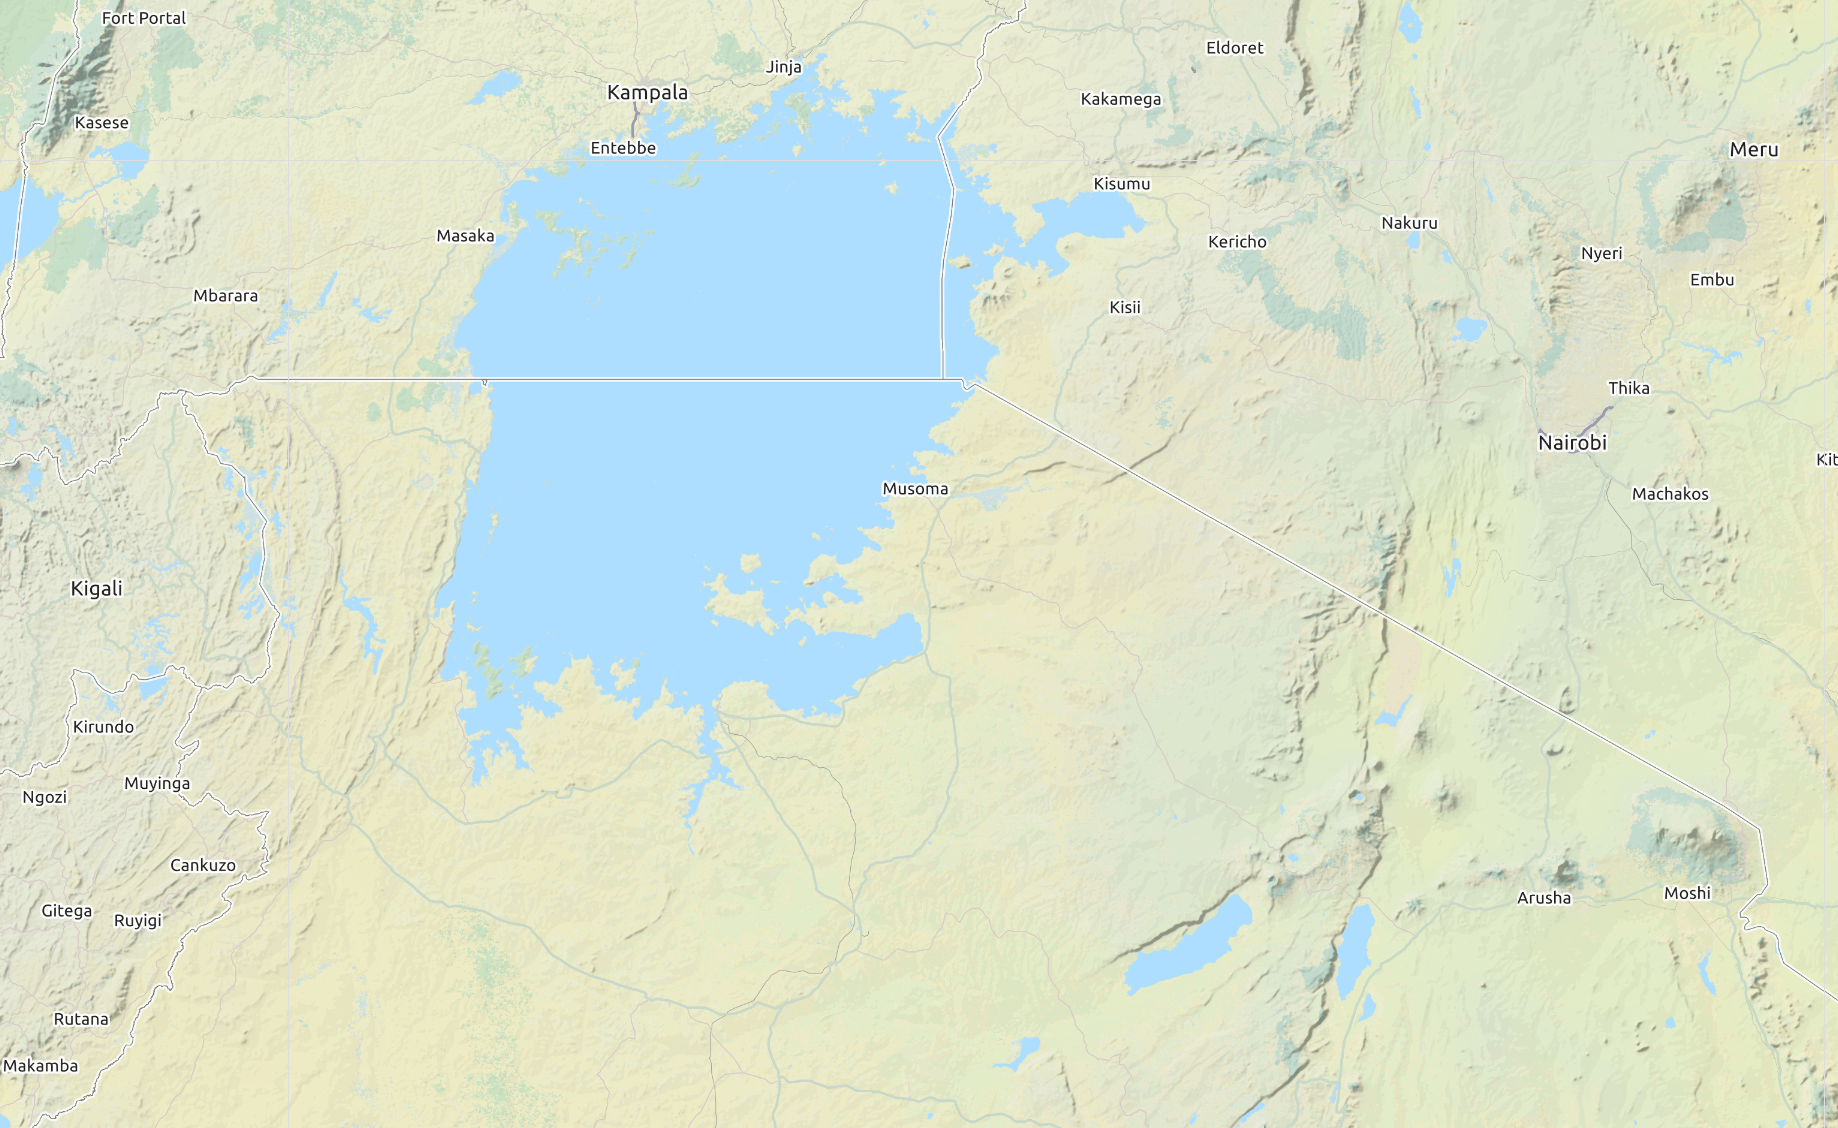
\includegraphics[width=0.9\textwidth]{chapter02/kigali.png}};
        \begin{scope}[x={(image.south east)},y={(image.north west)}]
            % 建立相对坐标系
            % \draw[help lines,xstep=.1,ystep=.1] (0,0) grid (1,1);
            % \foreach \x in {0,1,...,9} { \node [anchor=north] at (\x/10,0) {0.\x}; }
            % \foreach \y in {0,1,...,9} { \node [anchor=east] at (0,\y/10) {0.\y}; }
            % 作图命令
            \node[above] (Nairobi) at (0.85,0.6) {Nairobi};
            \node[below] (Kigali) at (0.05,0.5) {Kigali};
            \node[above] (Kampala) at (0.25,0.8) {Kampala};
            \draw[blue,-latex,thick] (Nairobi) -- node[above]{506 km Northwest}(Kampala);
            \draw[purple,-latex,thick] (Kampala) -- node[above]{374 km Sorthwest}(Kigali);
            \draw[-latex,thick] (Nairobi) -- node[above]{751 km West}(Kigali);
            \draw[purple,-latex,thick] (Nairobi) -- node[above]{374 km Sorthwest} (0.65, 0.3);
        \end{scope}
    \end{tikzpicture}
    \caption{二维空间中线性相关向量的地理例子(基本方向粗略近似)}
\end{figure}
\end{example}

\begin{remark}
    以下性质在确定向量是否是线性无关是非常有用:
    \begin{itemize}
        \item $k$个向量不是线性相关就是线性无关, 没有第三种选择。
        \item 如果向量$\x_1,...,\x_k$中至少
              有一个向量是$\bs{0}$, 那他们就是线性相关。
              如果有两个向量相同也是这样的。
        \item 向量$\{\x_1,...,\x_k : \x_i \neq \bs{0}, i = 1, ...,k\}, k \geqslant 2$,
              线性相关, 当且仅当(至少)其中一个向量是其他向量的线性组合。
              特别地,如果一个向量是另一个向量的倍数,
              即$\x_i = \lambda \x_j$,
              $\lambda \in \R$
              那么集合$\{x_1,..., x_k : x_i \neq \bs{0}, i = 1, ..., k\}$
              是线性相关的。
        \item 一种检查向量$\x_1,...,\x_k \in V$是否线性无关的特殊方法是使用高斯消元法:
              将所有向量写成矩阵 $\A$ 的列并进行高斯消元,直到矩阵为行阶梯形(这里不需要简约行阶梯形):
              \begin{itemize}
                  \item 主元列表示向量,它们与左侧的向量线性无关。
                        请注意,在构建矩阵时存在向量的排序。
                  \item 非主元列可以表示为其左侧主元列的线性组合。
                        例如,这个行阶梯形
                        \begin{equation}
                            \begin{bmatrix}
                                1 & 3 & 0 \\
                                0 & 0 & 2
                            \end{bmatrix}
                        \end{equation}
                        告诉我们第1,3列是主元列。
                        第2列是非主元列因为它是第1列的3倍。
              \end{itemize}
    \end{itemize}
    当且仅当所有列都是主元列时,所有列向量都是线性无关的。
    如果至少有一个非主元列,则这些列(以及相应的向量)是线性相关的。
    \hfill $\lozenge$
\end{remark}

\begin{example}
考虑$\R^4$与
\begin{equation}
    \x_1 =
    \begin{bmatrix}
        1 \\ 2 \\ -3 \\ 4
    \end{bmatrix},
    \x_2 =
    \begin{bmatrix}
        1 \\ 1 \\ 0 \\ 2
    \end{bmatrix},
    \x_3 =
    \begin{bmatrix}
        -1 \\ -2 \\ 1 \\ 1
    \end{bmatrix}.
\end{equation}
为了检查他们是否线性无关, 我们遵循一般方法并解
\begin{equation}
    \lambda_1\x_1 + \lambda_2\x_2 + \lambda_3\x_3 = \lambda_1
    \begin{bmatrix}
        1 \\ 2 \\ -3 \\ 4
    \end{bmatrix} +
    \lambda_2
    \begin{bmatrix}
        1 \\ 1 \\ 0 \\ 2
    \end{bmatrix} +
    \lambda_3
    \begin{bmatrix}
        -1 \\ -2 \\ 1 \\ 1
    \end{bmatrix}
    =\bs{0}
\end{equation}
我们用向量$\x_i,i = 1,2,3$作为一个矩阵的列并应用基本行操作, 直到我们确定主元列:
\begin{equation}
    \begin{bmatrix}
         1 &  1 & -1 \\
         2 &  1 & -2 \\
        -3 &  0 &  1 \\
         4 &  2 &  1 \\
    \end{bmatrix}
    \quad \rightsquigarrow \cdots \rightsquigarrow \quad
    \begin{bmatrix}
         1 &  1 & -1 \\
         0 &  1 &  0 \\
         0 &  0 &  1 \\
         0 &  0 &  0 \\
    \end{bmatrix}.
\end{equation}
这里,矩阵的每一列都是一个主元列。
因此,不存在非平凡解,我们用
$\lambda_1 = 0,\lambda_2 = 0,\lambda_3 = 0$ 来求解方程组。
因此,向量$\x_1,\x_2,\x_3$是线性无关的。
\end{example}

\begin{remark}
    考虑向量空间$V$
    考虑具有$k$个线性无关向量
    $\b_1,...,\b_k$
    的向量空间$V$。
    和$m$个线性组合
    \begin{equation}
    \begin{aligned}
        \x_1 &= \sum_{i=1}^{k}\lambda_{i1}\b_i, \\
                         &\vdots \\
        \x_m &= \sum_{i=1}^{k}\lambda_{im}\b_i, \\
    \end{aligned}
    \end{equation}
    定义$\B = [\b_1,...,\b_k]$
    为矩阵, 其中每一列都是线性独立的向量$\b_1,...,\b_k$, 我们用
    \begin{equation}
        \x_j = \bs{B\lambda}_j,
        \quad
        \bs{\lambda}_j =
        \begin{bmatrix}
            \lambda_{1j} \\
            \vdots \\
            \lambda_{kj} \\
        \end{bmatrix},
        \quad
        j = 1,..., m,
    \end{equation}
    来更简洁的表示他们。

    我们想要测试
    $\x_1,..., \x_m$
    是否线性独立。
    为此,我们遵循当
    $\sum_{j=1}^{m}\psi_j\x_j = \bs{0}$
    时的一般检验方法。
    根据 (2.71),我们得到
    \begin{equation}
       \sum_{j=1}^{m}\psi_j\x_j
       =
       \sum_{j=1}^{m}\psi_j\B\bs{\lambda}_j
       =
       \B\sum_{j=1}^{m}\psi_j\bs{\lambda_j}
    \end{equation}
    这意味着
    $\{\x_1,..., \x_m\}$
    线性无关当且仅当列向量
    $\{\bs{\lambda}_1,..., \bs{\lambda}_m\}$是线性无关的。
    \hfill $\lozenge$
\end{remark}

\begin{remark}
    在向量空间$V$中,
    k个向量$\x_1,...,\x_k$的$m$个线性组合
    是线性相关的, 如果$m > k$. \hfill $\lozenge$
\end{remark}

\begin{example}
考虑一组线性无关向量
$\b_1,\b_2,\b_3,\b_4 \in \R^n$
并且
\begin{equation}
    \begin{aligned}
        \begin{array}{lllllllll}
            \x_1 &=&  \b_1   &-& 2\b_2  &+&\b_3    &-& \b_4 \\
            \x_2 &=&  -4\b_1 &-& 2\b_2  & &                    &+& 4\b_4 \\
            \x_3 &=&  2\b_1  &+& 3\b_2  &-&\b_3    &-& 3\b_4 \\
            \x_4 &=&  17\b_1 &-& 10\b_2 &+&11\b_3  &+& \b_4 \\
        \end{array}
    \end{aligned}
\end{equation}
向量$\x_1,...,\x_4 \in \R^n$线性独立吗?
为了回答这个问题, 我们调查列向量
\begin{equation}
    \left\{
    \begin{bmatrix}
        1 \\ -2 \\ 1 \\ -1
    \end{bmatrix},
    \begin{bmatrix}
        -4 \\ -2 \\ 0 \\ 4
    \end{bmatrix},
    \begin{bmatrix}
        2 \\ 3 \\ -1 \\ -3
    \end{bmatrix},
    \begin{bmatrix}
        17 \\ -10 \\ 11\\ 1
    \end{bmatrix}
    \right\}
\end{equation}
是否是线性独立的。
对应线性方程组的系数矩阵
\begin{equation}
    \A=
    \begin{bmatrix}
        1 & -4 & 2 & 17 \\
        -2 & -2 & 3 & 10 \\
        1 & 0 & -1 & 11 \\
        -1 & 4 & -3 & 1 \\
    \end{bmatrix}
\end{equation}
其简约行阶梯形矩阵
\begin{equation}
    \begin{bmatrix}
        1 & 0 & 0 & -7 \\
        0 & 1 & 0 & -15 \\
        0 & 0 & 1 & -18 \\
        0 & 0 & 0 & 0 \\
    \end{bmatrix}
\end{equation}
我们看到相应的线性方程组是非平凡可解的:
最后一列不是主元列,并且
$\x_4 = −7\x_1 −15\x_2 −18\x_3$。
因此,$\x_1,..., \x_4$是线性相关的,
因为$\x_4$可以表示为$\x_1,...,\x_3$的线性组合。
\end{example}

\section{基与秩}

在向量空间$V$中,我们对向量集合$\mc{A}$特别感兴趣,这些向量集合具有性质:
任何向量$\bs{v} \in V$可以通过$\mc{A}$中向量的线性组合获得。
这些向量是特殊的向量,接下来,我们将表征它们。

\subsection{生成集合与基}

\begin{definition}[生成集合与张成]
    考虑向量空间$V=(\mc{V,+,\cdot})$
    和一组向量$\mc{A}=\{\x_1,...,\x_k\} \subseteq \mc{V}$.
    如果任意向量$\bs{v}\in \mc{V}$能够表示为
    $\x_1,...,\x_k$的线性组合,
    $\mc{A}$称作$V$的一个生成集合(generating set).
    $\mc{A}$向量的所有线性组合的集合称为$\mc{A}$的张成(span).
    如果$\mc{A}$张成向量空间$V$, 我们写作
    $V = \mathrm{span}[\mc{A}]$ 或者
    $V = \mathrm{span}[\x_1,...,\x_k]$.
\end{definition}

生成集合是张成向量(子)空间的向量集,
即每个向量都可以表示为生成集中向量的线性组合。
现在,我们将更具体地描述张成向量(子)空间的最小生成集。

\begin{definition}[基].
    考虑向量空间$V=(\mc{V,+,\cdot})$
    和$\mc{A} \subseteq \mc{V}$.
    $V$的生成集合$\mc{A}$称为最小的(minimal)
    如果不存在更小的集合
    $\tilde{\mc{A}}\subsetneq\mc{A}\subseteq\mc{V}$
    张成$V$.
    任意线性无关的生成集合都是最小的, 称作$V$的基(basis).
\end{definition}

令$V = (\mc{V},+,\cdot)$为向量空间并且
$\mc{B} \subseteq \mc{V}, \mc{B} \neq \emptyset$.
那么, 下面的陈述是等价的:
\begin{itemize}
    \item $\mc{B}$是$V$的一个基。
    \item $\mc{B}$是一个最小生成集合。
    \item $\mc{B}$是$V$中的最大线性无关向量集,添加集合外的任何其他向量将使其线性相关。
    \item 任意向量$\x \in V$是
          $\mc{B}$中向量的线性组合,并且每个线性组合都是唯一的,i.e.
    \begin{equation}
        \x =
        \sum_{i=1}^{k}\lambda_i\b_i =
        \sum_{i=1}^{k}\psi_i\b_i
    \end{equation}
    其中,$\lambda_i, \psi_i \in \R,\b_i \in \mc{B}$
    它遵循$\lambda_i = \psi_i, i = 1,\dots,k$.
\end{itemize}

\begin{example}
    .
    \begin{itemize}
        \item $\R^3$中, 规范/标准基是
        \begin{equation}
            \mc{B} = \left\{
                \begin{bmatrix} 1 \\ 0 \\ 0 \end{bmatrix},
                \begin{bmatrix} 0 \\ 1 \\ 0 \end{bmatrix},
                \begin{bmatrix} 0 \\ 0 \\ 1 \end{bmatrix}
            \right\}
        \end{equation}
        \item $\R^3$中不同的基
        \begin{equation}
           \mc{B}_1 = \left\{
                \begin{bmatrix} 1 \\ 0 \\ 0 \end{bmatrix},
                \begin{bmatrix} 1 \\ 1 \\ 0 \end{bmatrix},
                \begin{bmatrix} 1 \\ 1 \\ 1 \end{bmatrix}
            \right\},
            \mc{B}_2 = \left\{
                \begin{bmatrix} 0.5 \\ 0.8 \\ 0.4 \end{bmatrix},
                \begin{bmatrix} 1.8 \\ 0.3 \\ 0.3 \end{bmatrix},
                \begin{bmatrix} -2.2 \\ -1.3 \\ 3.5 \end{bmatrix}
            \right\}.
        \end{equation}
        \item 集合
        \begin{equation}
           \mc{A} = \left\{
               \begin{bmatrix}
                   1 \\ 2 \\ 3 \\ 4
               \end{bmatrix},
               \begin{bmatrix}
                   2 \\ -1 \\ 0 \\ 2
               \end{bmatrix},
               \begin{bmatrix}
                   1 \\ 1 \\ 0 \\ -4
               \end{bmatrix}
           \right\}
        \end{equation}
        是线性独立的, 但是不是一个生成集合(也不是基):
        例如,向量$[1, 0, 0, 0]^\top$不能通过$\mc{A}$中元素的线性组合获得。
    \end{itemize}
\end{example}

\begin{remark}
    每个向量空间$V$都有一个基$\mc{B}$。
    前面的例子表明向量空间$V$可以有很多基,即没有唯一的基。
    但是,所有基都具有相同数量的元素,即基向量(basis vectors)
    \hfill $\lozenge$
\end{remark}

我们只考虑有限维向量空间$V$。
在这种情况下,$V$的维数是$V$的基向量的数量,我们写成$\dim(V)$。
如果$U \subseteq V$是$V$的子空间,则$\dim(U) \leqslant \dim(V)$
并且当且仅当$U=V$时, $\dim(U) = \dim(V)$.
直觉上,向量空间的维数可以被认为是这个向量空间中独立方向的数量。

\begin{remark}
    向量空间的维数不必是向量中的元素数。
    举个例子, 向量空间
    $V = \spn [\begin{bmatrix} 0 \\ 1 \end{bmatrix}]$
    是一维的, 尽管向量拥有两个元素。\hfill $\lozenge$
\end{remark}

\begin{remark}
   子空间$U$的基$\spn[\bs{x}_1,...,\bs{x}_m] \subseteq \mb{R}^n$
   可以通过执行以下步骤找到:
   \begin{enumerate}
       \item 将张成向量(spanning vectors)写成矩阵$\bs{A}$的列
       \item 确定$\bs{A}$的REF
       \item 与主元列关联的张成向量是$U$的基。
   \end{enumerate}
   \hfill $\lozenge$
\end{remark}

\begin{example}[确定基]
    对于向量子空间$U \subseteq \mb{R}^5$, 被以下向量张成
    \begin{equation}
        \bs{x}_1=
        \begin{bmatrix}
            1 \\ 2 \\ -1 \\ -1 \\ -1
        \end{bmatrix},
        \bs{x}_2=
        \begin{bmatrix}
            2 \\ -1 \\ 1 \\ 2 \\ -2
        \end{bmatrix},
        \bs{x}_3=
        \begin{bmatrix}
            3 \\ -4 \\ 3 \\ 5 \\ -3
        \end{bmatrix},
        \bs{x}_4=
        \begin{bmatrix}
            -1 \\ 8 \\ -5 \\ -6 \\ 1
        \end{bmatrix}
        \in \mb{R}^5,
    \end{equation}
    我们想要找出哪些向量$\bs{x}_1 ,..., \bs{x}_4$是$U$的基。
    为此,我们需要检查$\bs{x}_1 ,..., \bs{x}_4$是否线性无关。
    因此,我们需要解
    \begin{equation}
        \sum_{i=1}^{4} \lambda_i \bs{x}_i = \bs{0},
    \end{equation}
    于是有齐次方程组,其矩阵
    \begin{equation}
        \begin{bmatrix}
            \bs{x}_1 & \bs{x}_2 & \bs{x}_3 & \bs{x}_4
        \end{bmatrix} =
        \begin{bmatrix}
           1 & 2 & 3 & -1 \\
           2 & -1 & -4 & 8 \\
          -1 & 1 & 3 & -5 \\
          -1 & 2 & 5 & -6 \\
          -1 & -2 & -3 & 1 \\
        \end{bmatrix}
    \end{equation}
    根据线性方程组的基本变换规则,我们得到行阶梯形矩阵
    \[
        \begin{bmatrix}
           1 & 2 & 3 & -1 \\
           2 & -1 & -4 & 8 \\
          -1 & 1 & 3 & -5 \\
          -1 & 2 & 5 & -6 \\
          -1 & -2 & -3 & 1 \\
        \end{bmatrix}
        \quad \rightsquigarrow \cdots \rightsquigarrow \quad
        \begin{bmatrix}
           1 & 2 & 3 & -1 \\
           0 & 1 & 2 & -2 \\
           0 & 0 & 0 & 1 \\
           0 & 0 & 0 & 0 \\
           0 & 0 & 0 & 0 \\
        \end{bmatrix}
    \]
    由于主元列表示哪组向量线性无关,
    我们从行阶梯梯形矩阵中看出$\bs{x}_1 , \bs{x}_2 , \bs{x}_4$
    是线性无关的
    (因为线性方程组
    $\lambda_1\bs{x}_1 + \lambda_2\bs{x}_2 + \lambda_4\bs{x}_4 = \bs{0}$
    只能求解为$\lambda_1 = \lambda_2 = \lambda_4 = 0)$。
    因此, $\{\bs{x}_1, \bs{x}_2, \bs{x}_4\}$ 是$U$的基。
\end{example}

\subsection{秩}

矩阵$\bs{A}\in \mb{R}^{m×n}$的线性无关列数等于线性无关行数,
称为$\bs{A}$的秩,记为$\rk(\bs{A})$.\marginpar{秩}

\begin{remark}
    矩阵的秩有一些重要的性质:
    \begin{itemize}
    \item $\rk(\bs{A}) = \rk(\bs{A}^\top)$,即列秩等于行秩。
    \item $\bs{A} \in \mb{R}^{m\times n}$的列
           张成一个子空间$U \subseteq \R^{m\times n}$
           且$\dim(U) = \rk(\bs{A})$.
           稍后我们将把这个子空间称为像(image)或范围(range)。
           可以通过对$\bs{A}$应用高斯消元法来确定主元列,从而找到$U$的基。
    \item $\bs{A} \in \mb{R}^{m\times n}$的行张成子空间
          $W \subseteq \R^n$, 且$\dim(W) = \rk(\bs{A})$.
          $W$的基可以通过对$\bs{A}^\top$应用高斯消元法来找到。
    \item 对于所有$\bs{A} \in \R^{n \times n}$,$\bs{A}$是正规的(可逆的)当且仅当$\rk(\bs{A}) = n$。
    \item 对于所有$\bs{A} \in \mb{R}^{m\times n}$
          和所有 $\bs{b} \in \mb{R}^{m\times n}$
          当且仅当$\rk(\bs{A}) = \rk(\bs{A}|b)$时,
          线性方程组$\A\x = \bs{b}$有解,其中$\bs{A}|\bs{b}$表示增广矩阵。。
    \item 对于$\bs{A} \in \mb{R}^{m\times n}$,
          $\A\x = \bs{0}$的解的子空间维度为
          $n − \rk(\bs{A})$。
          稍后,我们将称这个子空间为核(kernel)或零(null)空间。
    \item 如果矩阵$\bs{A} \in \R^{m\times n}$的秩等于相同维度矩阵的最大可能秩,则该矩阵具有满秩。
          这意味着满秩矩阵的秩是行数和列数中的较小者,即$\rk(A) = \min(m,n)$。
          如果矩阵没有满秩,则称该矩阵是秩亏的(rank deficient)。
    \end{itemize}
    \hfill $\lozenge$
\end{remark}

\begin{example}[秩].\\
    \begin{itemize}
        \item $\A =
        \begin{bmatrix}
            1 & 0 & 1 \\
            0 & 1 & 1 \\
            0 & 0 & 0
        \end{bmatrix}$.
        $\A$有两个线性无关行/列, 所以$\rk(\A) = 2$.
        \item $\A =
        \begin{bmatrix}
            1 & 2 & 1 \\
            -2 & -3 & 1 \\
            3 & 5 & 0
        \end{bmatrix}$
        我们使用高斯消元法来确定秩:
        \begin{equation}
            \begin{bmatrix}
                1 & 2 & 1 \\
                -2 & -3 & 1 \\
                3 & 5 & 0
            \end{bmatrix}
            \quad \rightsquigarrow\cdots\rightsquigarrow\quad
            \begin{bmatrix}
                1 & 2 & 1 \\
                0 & 1 & 3 \\
                0 & 0 & 0
            \end{bmatrix}.
        \end{equation}
        这里, 我们看到线性无关的行列都是$2$, 所以$\rk(\A) = 2$.
    \end{itemize}
\end{example}

\section{线性映射}

接下来,我们将研究保留其结构的向量空间上的映射(mappings),这将使我们能够定义坐标(coordinate)的概念。
在本章的开头,我们说过向量是可以相加并乘以标量的对象,结果对象仍然是向量。
我们希望在应用映射时保留这个属性:考虑两个实向量空间(real vector spaces)$V, W$。
映射$\Phi : V \rightarrow W$保留向量空间的结构,如果
\begin{align}
    \Phi(\x + \y) &= \Phi(\x) + \Phi(y) \\
    \Phi(\lambda\x) &= \lambda\Phi(\x)
\end{align}
对于所有$\x,\y \in V$和$\lambda \in \R$.
我们将其总结为如下定义:
\begin{definition}[线性映射].
   对于向量空间$V,W$, 线性映射$\Phi:V\rightarrow W$称为线性映射
   (或向量空间同态(vector space homomorphism)/线性变换(linear transformation))如果
   \begin{equation}
       \forall \x,\y \in V \forall \lambda,\psi \in \R:
       \Phi(\lambda\x + \psi \y) = \lambda \Phi(\x) + \psi \Phi(\y)
   \end{equation}
\end{definition}

事实证明,我们可以将线性映射表示为矩阵(第 2.7.1 节)。
回想一下,我们还可以收集一组向量作为矩阵的列。
在处理矩阵时,我们必须记住矩阵代表什么:线性映射或向量集合。
我们将在第 4 章中看到更多关于线性映射的内容。
在继续之前,我们将简要介绍特殊映射。

\begin{definition}[单射、满射、双射].
    考虑映射$\Phi:V \rightarrow W$,其中$V, W$可以是任意集合。
    那么$\Phi$被称为
    \begin{itemize}
        \item 单射:如果$\forall \x,\y \in \mc{V}:
               \Phi(\x) = \Phi(\y) \Longrightarrow \x = \y$.
        \item 满射:如果$\Phi(\mc{V})=\mc{W}$.
        \item 双射:如果它既是单射, 也是满射。
    \end{itemize}
\end{definition}

如果$\Phi$是满射,那么$\mc{W}$中的每个元素都可以使用$\Phi$从$\mc{V}$"获得"。
双射$\Phi$可以“撤销(undone)”,即存在映射$\Psi:\mc{W} \rightarrow \mc{V}$
使得$\Psi \circ \Phi(\x) = \x$.
这个映射$\Psi$被称为$\Phi$的逆,通常用$\Phi^{−1}$表示。

通过这些定义,我们介绍向量空间$V$和$W$间线性映射的特殊情况:
\begin{itemize}
    \item 同构(Isomorphism)\marginpar{Isomorphism}   :$\Phi:V \rightarrow W$线性和双射
    \item 内同态(Endomorphism)\marginpar{Endomorphism}:$\Phi:V \rightarrow V$线性
    \item 自同构(Automorphism)\marginpar{Automorphism}:$\Phi:V \rightarrow V$线性和双射
    \item 我们将 $\mathrm{id}_V:V \rightarrow V ,\x \mapsto \x$
          定义为$V$中的恒等映射(identity mapping)或恒等自同构(identity automorphism)。
\end{itemize}

\begin{example}[同态]
    映射$\Phi:\R^2 \rightarrow \mb{C}, \Phi(\x) = x_1 + ix_2$是同态(homomorphism):
    \begin{equation}
        \begin{aligned}
            \Phi\left(
                \begin{bmatrix} x_1 \\ x_2 \end{bmatrix} +
                \begin{bmatrix} y_1 \\ y_2 \end{bmatrix}
                \right) &=
            (x_1 + y_1) + i(x_2 + y_2) = x_1 + ix_2 + y_1 + iy_2 \\
            &= \Phi \left(\begin{bmatrix} x_1 \\ x_2 \end{bmatrix}\right)
            + \Phi \left(\begin{bmatrix} y_1 \\ y_2 \end{bmatrix}\right) \\
            \Phi\left(\lambda \begin{bmatrix} x_1 \\ x_2 \end{bmatrix}\right)
            &= \lambda x_1 + \lambda i x_2 = \lambda(x_1+ix_2)
            = \lambda \Phi\left(\begin{bmatrix} x_1 \\ x_y \end{bmatrix}\right)
        \end{aligned}
    \end{equation}
    这也证明了为什么可以将复数表示为$\R^2$中的元组:
    存在双射线性映射,可将$\R^2$中元组的元素加法转换为具有对应加法的复数集。
    请注意,我们只显示了线性,而不是双射。
\end{example}

\begin{theorem}[Theorem 3.59 in Axler(2015)]
    有限维向量空间$V$和$W$是同构的当且仅当$\dim(V) = \dim(W)$.
\end{theorem}

定理 2.17 指出在两个相同维度的向量空间之间存在线性双射映射。
直观上,这意味着相同维度的向量空间是一种相同的东西,
因为它们可以相互转换而不会产生任何损失。

定理 2.17 也给出了将$\R^{m×n}$($m\times n$矩阵的向量空间)
和$\R^{mn}$(长度为$mn$的向量的向量空间)视为相同的理由,
因为它们的维数是$mn$,并且存在线性的将一个转换为另一个的双射映射。

\begin{remark}
    考虑向量空间$V,W,X$, 那么:
    \begin{itemize}
        \item 对于线性映射$\Phi:V \rightarrow W$和$\Psi:W \rightarrow X$,
              映射$\Psi \circ \Phi:V \rightarrow X$也是线性的。
        \item 如果$\Phi:V \rightarrow W$是同构,那么$\Phi^{−1}:W \rightarrow V$也是同构。
        \item 如果$\Phi:V \rightarrow W, \Psi:V\rightarrow W$是线性的, 那么
              $\Phi + \Psi$和$\lambda \Phi, \lambda \in \R$也是线性的
              \hfill $\lozenge$
    \end{itemize}
\end{remark}

\subsection{线性映射的矩阵表示}

任何$n$-维向量空间与$\R^n$同构(定理 2.17)。
我们考虑一个基${\b_1 ,..., \b_n}$的$n$-维向量空间$V$。
接下来,基向量的顺序将很重要。
因此,我们令
\begin{equation}
    B = (\b_1,\dots,\b_n)
\end{equation}
并且称该$n$-元组为$V$的一个有序基(ordered basis).

\begin{remark}[符号]。
    我们正处于符号变得有点棘手的地步。
    因此,我们在这里总结一部分。
    $B = (\b_1,\dots, \b_n)$是有序基,
    $\mc{B} = \{\b_1,\dots, \b_n\}$是一个(无序)基,
    $\B = [\b_1,\dots, \b_n ]$是一个矩阵,
    其列是向量$\b_1,\dots,\b_n$.
\end{remark}

\begin{definition}[坐标(coordinates)]
    考虑向量空间$V$和$V$的一个有序基$B = (\b_1,\dots, \b_n)$.
    对于所有$\x \in V$,我们得到一个$\x$相对于$B$的唯一的表示(线性组合)
    \begin{equation}
        \x = \alpha_1\b_1 + \dots + \alpha_n\b_n
    \end{equation}
    那么, $\alpha_1,\dots,\alpha_n$是$\x$相对于B的坐标,并且向量
    \begin{equation}
        \bs{\alpha} =
        \begin{bmatrix}
            \alpha_1 \\ \vdots \\ \alpha_n
        \end{bmatrix}
        \in \R^n
    \end{equation}
    是$\x$相对于有序基$B$的坐标向量/坐标表示
\end{definition}

\begin{figure}
    \begin{tikzpicture}[ultra thick, -latex]
        \draw[help lines, blue,thin] (-0.5,-0.5) grid (5.5,5.5);
        \draw[blue] (0,0) -- (1,0) node[below]{$e_1$};
        \draw[blue] (0,0) -- (0,1) node[left]{$e_2$};
        \draw[black] (0,0) -- (2,2) node[right]{$x$};
    \end{tikzpicture}
    \begin{tikzpicture}[ultra thick, -latex]
        \draw[help lines, blue,thin] (-0.5,-0.5) grid (5.5,5.5);
        \draw[blue] (0,0) -- (1.5,0.5) node[below]{$b_1$};
        \draw[blue] (0,0) -- (0.5,1.5) node[left]{$b_2$};
        \draw[black] (0,0) -- (2,2) node[right]{$x$};
    \end{tikzpicture}
    \caption{由两组基向量定义的两个不同坐标系。
    根据选择的坐标系,向量$\x$具有不同的坐标表示。}
\end{figure}

一个基有效地定义了一个坐标系(coordinate system)。
我们熟悉二维笛卡尔坐标系(Cartesian coordinate system in two dimensions),
它由规范基向量$\e_1,\e_2$张成。
在这个坐标系中,向量$\x \in \R^2$有一个表示,
它告诉我们如何线性组合$\e_1$和$\e_2$以获得$\x$。
然而,$\R^2$的任何基定义了一个有效的坐标系,
并且之前的相同向量$\x$在$(\b_1, \b_2)$基中可能具有不同的坐标表示。
在图 2.8 中,$x$相对于标准基$(\e_1, \e_2)$的坐标是$[2, 2]^\top$。
然而,对于基$(\b_1, \b_2)$,相同的向量$\x$表示为$[1.09, 0.72]^\top$,
即$\x = 1.09\b_1 + 0.72\b_2$。
在下面的部分中,我们将发现如何获得这种表示。

\begin{example}
    让我们看一下几何向量$\x \in \R^2$,
    其相对于$\R^2$的标准基$(\e_1 , \e_2)$的坐标为$[2, 3]^\top$。
    这意味着,我们可以写出$\x = 2\e_1 + 3\e_2$。
    然而,我们不必选择标准基来表示这个向量。
    如果我们使用基向量$\b_1 = [1, -1]^\top, \b_2 = [1, 1]^\top$
    我们将得到坐标$\frac{1}{2}[-1, 5]^\top$来表示相同的向量,
    这是相对于$(\b_1, \b_2)$(见图 2.9)。
\end{example}

\begin{figure}[H]
    \begin{tikzpicture}[-latex,thick]
        \draw[blue] (0,0) -- (1,0) node[below]{$e_1$};
        \draw[blue] (0,0) -- (0,1) node[left]{$e_2$};
        \draw[orange] (0,0) -- (1,-1) node[above right]{$b_1$};
        \draw[orange] (0,0) -- (1,1) node[below right]{$b_2$};
        \draw[black] (0,0) -- (2,3);
        \node [blue] at (-1,3) {$\x = 2\e_1 + 3\e_2$};
        \node [orange] at (-1,2) {$\x = -\frac{1}{2}\b_1 + \frac{5}{2}\b_2$};
    \end{tikzpicture}
    \caption{向量$\x$的不同坐标表示,取决于基的选择。}
\end{figure}

\begin{remark}
    对于 n 维向量空间$V$和$V$的有序基$B$,
    映射$\Phi:\R^n \rightarrow V, \Phi(\e_i) = \b_i, i = 1,\dots, n$是线性的
    (并且由于定理 2.17 是同构的),
    其中$(\e_1,\dots,\e_n)$是$\R^n$的标准基。
    \hfill $\lozenge$
\end{remark}

现在我们准备在矩阵和有限维向量空间之间的线性映射之间建立明确的联系。

\begin{definition}[变换矩阵]
    考虑向量空间$V, W$具有相应的(有序)基
    $B = (\b_1,\dots,\b_n)$和$C = (\c_1,\dots, \c_m )$。
    此外,我们考虑线性映射$\Phi:V \rightarrow W$。
    对于$j \in \{1,\dots, n\}$,
    \begin{equation}
        \Phi(\b_j) = \alpha_{1j}\c_1 + \cdots + \alpha_{mj}\c_m
        = \sum_{i=1}^{m}\alpha_{ij}\c_i
    \end{equation}
    是$\Phi(\b_j)$关于$C$的唯一表示。
    然后,我们称$m \times n$-矩阵$\A_\Phi$,其元素由下式给出
    \begin{equation}
        A_\phi(i,j) = \alpha_{ij},
    \end{equation}
    为$\Phi$的变换矩阵(Transformation Matrix)(相对于$V$的有序基$B$和$W$的有序基$C$)。
\end{definition}

$\Phi(\b_j)$相对于$W$的有序基$C$的坐标是$\A_\Phi$的第$j$列。
考虑(有限维)向量空间$V,W$具有有序基$B,C$和线性映射$\Phi:V \rightarrow W$及其变换矩阵$A_\Phi$。
如果$\hat{\x}̂$ 是 $\x \in V$相对于$B$的坐标向量,
$\hat{\y}$是$\y = \Phi(\x) \in W$相对于$C$的坐标向量,那么
\begin{equation}
    \hat{\y} = \A_\Phi \hat{\x}
\end{equation}
这意味着变换矩阵可用于将关于$V$中有序基的坐标映射到关于$W$中有序基的坐标。

\begin{example}[变换矩阵]
    考虑同态$\Phi:V \rightarrow W$和
    $V$的有序基$B = (\b_1,\dots, \b_3)$和
    $W$的有序基$C = (\c_1,\dots, \c_4)$。
    \begin{equation}
        \begin{aligned}
            \Phi(\b_1) &= \c_1  - \c_2 + 3\c_3 -  \c_4 \\
            \Phi(\b_2) &= 2\c_1 + \c_2 + 7\c_3 + 2\c_4 \\
            \Phi(\b_2) &=       3\c_2 +  \c_3 + 4\c_4 \\
        \end{aligned}
    \end{equation}
    关于B和C的变化矩阵$\A_\Phi$满足
    $\Phi(\b_k) = \sum_{1=1}^{4}\alpha_{ik}\c_i$
    其中$k=1,\dots,3$, 并给出
    \begin{equation}
        \A_\Phi =
        [\bs{\alpha}_1,\bs{\alpha}_2,\bs{\alpha}_3]=
        \begin{bmatrix}
            1 & 2 & 0 \\
            -1 & 1 & 3 \\
            3 & 7 & 1 \\
            -1 & 2 & 4
        \end{bmatrix},
    \end{equation}
    其中$\bs{\alpha}_j,j = 1, 2, 3$是$\Phi(\b_j)$相对于$C$的坐标向量。
\end{example}

\begin{example}[向量的线性变换]
    \begin{figure}[H]
        \subfigure[原始数据]{
            \begin{tikzpicture}
                \draw (-1,0) -- (1,0);
                \draw (0,-1) -- (0,1);
            \end{tikzpicture}
        }
        \subfigure[旋转45度]{
            \begin{tikzpicture}
                \draw (-1,0) -- (1,0);
                \draw (0,-1) -- (0,1);
            \end{tikzpicture}
        }
        \subfigure[伸缩水平轴]{
            \begin{tikzpicture}
                \draw (-1,0) -- (1,0);
                \draw (0,-1) -- (0,1);
            \end{tikzpicture}
        }
        \subfigure[一般线性映射]{
            \begin{tikzpicture}
                \draw (-1,0) -- (1,0);
                \draw (0,-1) -- (0,1);
            \end{tikzpicture}
        }
        \caption{(a) 中用点表示的向量线性变换的三个例子;}
    \end{figure}
    我们考虑$R^2$中一组向量的三个线性变换,其变换矩阵为
    \begin{equation}
        \A_1 =
        \begin{bmatrix}
            \cos(\frac{\pi}{4}) & -\sin(\frac{\pi}{4}) \\
            \sin(\frac{\pi}{4}) & \cos(\frac{\pi}{4})
        \end{bmatrix},
        \A_2 =
        \begin{bmatrix}
            2 & 0 \\
            0 & 1
        \end{bmatrix},
        \A_3 =
        \frac{1}{2}
        \begin{bmatrix}
            3 & -1 \\
            1 & -1
        \end{bmatrix}.
    \end{equation}
    图 2.10 给出了一组向量的线性变换的三个例子。
    图 2.10(a) 显示了$\R^2$中的 400 个向量,每个向量由相应$(x_1 , x_2 )$坐标处的点表示。
    矢量排列在一个正方形中。
    当我们使用(2.97)中的矩阵$\A_1$对这些向量中的每一个进行线性变换时,我们得到图 2.10(b)中的旋转正方形。
    如果我们应用由$\A^2$表示的线性映射, 我们将获得图 2.10(c) 中的矩形, 其中每个$x_1$坐标被拉伸 2倍。
    图 2.10(d) 显示了使用$\A_3$进行线性变换时图 2.10(a) 中的原始正方形, 它是反射、旋转和拉伸的组合。
\end{example}

\subsection{变基/基变换(basis change)}

接下来,我们将仔细研究如果我们改变$V$和$W$中的基,
线性映射$\Phi:V \rightarrow W$的变换矩阵如何改变的。
考虑$V$的两个有序基
\begin{equation}
    B = (\b_1,\dots,\b_n),\quad
    \tilde{B} = (\tilde{\b}_1,\dots,\tilde{\b}_n)
\end{equation}
和$W$的两个有序基
\begin{equation}
    C = (\c_1,\dots,\c_m),\quad
    \tilde{C} = (\tilde{\c}_1,\dots,\tilde{\c}_n)
\end{equation}
此外,$\A_\Phi \in \R^{m \times n}$是
线性映射$\Phi:V \rightarrow W$对基$B$和$C$的变换矩阵,
$\tilde{\A}_\Phi \in \R^{m \times n}$
是对$\tilde{B}$和$\tilde{C}$的对应变换映射。
我们将研究$\A$和$\tilde{}{\A}$是如何相互联系的,
即,如果我们选择执行从$B, C$到$\tilde{B}, \tilde{C}$的基变换,
我们如何/是否可以将$\A_\Phi$转换为$\tilde{\A}_\Phi$。
\begin{remark}
    我们有效地获得了恒等映射$\mathrm{id}_V$的不同坐标表示。
    在图2.9的上下文中,这意味着将关于$(\e_1,\e_2)$的坐标
    映射到关于$(\b_1, \b_2)$的坐标而不改变向量$\x$。
    通过改变基和相应的向量表示,
    关于这个新基的变换矩阵可以有一个特别简单的形式,
    可以允许直接计算。 \hfill $\lozenge$
\end{remark}

\begin{example}[基变换]
    考虑相对于$\R^2$中规范基的变换矩阵
    \begin{equation}
            \A =
        \begin{bmatrix}
            2 & 1 \\ 1 & 2
        \end{bmatrix}
    \end{equation}
    如果我们定义一个新基
    \begin{equation}
        B =(
        \begin{bmatrix} 1 \\ 1 \end{bmatrix},
        \begin{bmatrix} 1 \\ -1 \end{bmatrix}
        )
    \end{equation}
    我们得到一个相对于$B$的对角线变换矩阵
    \begin{equation}
        \tilde{\A}=
        \begin{bmatrix}
            3 & 0 \\ 0 & 1
        \end{bmatrix}
    \end{equation}
    这比$\A$更好用
\end{example}

在下文中,我们将研究将一个基的坐标向量转换为关于不同基的坐标向量的映射。
我们将首先陈述我们的主要结果,然后提供解释。

\begin{theorem}[基变换]
    对于线性映射$\Phi:V\rightarrow W$,$V$的有序基
    \begin{equation}
        B = (\b_1, \dots, \b_n),\quad
        \tilde{B} = (\tilde{\b}_1, \dots, \tilde{\b}_n)
    \end{equation}
    和$W$的有序基
    \begin{equation}
        C = (\c_1, \dots, \c_n),\quad
        \tilde{C} = (\tilde{\c}_1, \dots, \tilde{\c}_n)
    \end{equation}
    以及关于$B$和$C$的变换矩阵$\A_\Phi$,
    关于$\tilde{B}$和$\tilde{C}$的变换矩阵$\tilde{\A}_\Phi$
    \begin{equation}
        \tilde{\A}_\Phi = \bs{T}^{-1}\A_\Phi\bs{S}.
    \end{equation}
    这里,$\bs{S} \in \R^{n \times n}$是$\id_V$的变换矩阵,
    将关于$\tilde{B}$的坐标映射到关于$B$的坐标,
    $\bs{T} \in \R^{m \times m}$是$\id_W$的变换矩阵,
    将关于$\tilde{C}$的坐标映射到$C$的坐标。
\end{theorem}

\begin{proof}
    根据Drumm 和 Weil (2001),
    我们可以将$V$的新基$\tilde{B}$的向量写成$B$的基向量的线性组合,
    使得
    \begin{equation}
        \tilde{\b}_j = s_{1j}\b_1 + \cdots + s_{nj}\b_n =
        \sum_{i=1}^{n} s_{ij}\b_{j},
        \quad j = 1,\dots, n.
    \end{equation}
    类似的,我们将$W$的新基向量$\tilde{C}$写成$C$的基向量的线性组合,得到
    \begin{equation}
        \tilde{\c}_k = t_{1k}\c_1 + \cdots + t_{mk}\c_m =
        \sum_{l=1}^{n} t_{lk}\c_{l},
        \quad k = 1,\dots, m.
    \end{equation}
    我们将$\bs{S}=((s_{ij})) \in \R^{n \times n}$
    定义为将关于$\tilde{B}$的坐标映射到关于$B$的坐标的变换矩阵,
    $\bs{T}= ((t_{lk})) \in \R ^ {m\times m}$作为将关于$\tilde{C}$的坐标映射到到关于$C$的坐标。
    特别地,$\bs{S}$的第$j$列是$\tilde{\b}_j$相对于$B$的坐标表示,
    $\bs{T}$的第k列是$\tilde{\c}_k$相对于$C$的坐标表示。
    请注意,$\bs{S}$和$\bs{T}$都是正规的。

    我们将从两个角度来看$\Phi(\tilde{\b}_j)$。
    首先,应用映射$\Phi$,我们得到所有$j = 1,\dots, n$
    \begin{equation}
        \Phi(\tilde{\b}_j) =
        \sum_{k=1}^{m}
        \underbrace{\tilde{a}_{kj} {\color{blue}\tilde{\c}_k}}_{\in W}
        \overset{(2.107)}{=}
        \sum_{k=1}^{m} \tilde{a}_{kj}
        {\color{blue} \sum_{l=1}^{m}t_{lk}\c_l}
        =
        \sum_{l=1}^{m}
        \left(
            \sum_{k=1}^{m} t_{lk} \tilde{a}_{kj}
        \right)
        \c_l,
    \end{equation}
    这里我们首先将新的基向量$\tilde{\c}_k \in W$
    表示为基向量$\c_l \in W$的线性组合,然后交换求和的顺序。

    或者,当我们将$\tilde{\b}_j \in V$表示为$\b_j \in V$的线性组合时,
    我们得到
    \begin{subequations}
        \begin{equation}
        \Phi({\color{blue}\tilde{\b}_j})
        \overset{(2.106)}{=}
        \Phi
        \left(
            {\color{blue}
            \sum_{i=1}^{n}s_{ij}\b_i
            }
        \right)
        =
        \sum_{i=1}^{n} s_{ij}
        {\color{red}
        \Phi(\b_i)
        }
        =
        \sum_{i=1}^{n} s_{ij}
        \sum_{l=1}^{m}
        {\color{red}
        a_{li} \c_l
        }
        \end{equation}
        \begin{equation}
        =
        \sum_{l=1}^{m} \left(\sum_{i=1}^{n}a_{li} s_{ij}\right)
        \c_l,\quad j = 1,\dots, n,
        \end{equation}
    \end{subequations}
   这里我们利用了$\Phi$的线性(linearity).比较(2.108)和(2.109b),
   它有: 对于所有$j=1,\dots,n$和$l=1,\dots,m$
   \begin{equation}
       \sum_{k=1}^{m}t_{lk} \tilde{a}_{kj} =
       \sum_{i=1}^{n}a_{li} {s}_{ij}
   \end{equation}
   因此:
   \begin{equation}
       \T\tilde{\A}_\Phi = \A_\Phi\bs{S}\in \R^{m \times n},
   \end{equation}
   使得
   \begin{equation}
       \tilde{\A}_\Phi = \T^{-1} \A_\Phi \bs{S},
   \end{equation}
   这就证明了定理2.20. \hfill $\square$
\end{proof}

定理 2.20 告诉我们,
随着$V$($B$替换为 $\tilde{B}$)和$W$($C$ 替换为 $\tilde{C}$)的基变化,
线性映射$\Phi:V \rightarrow W$的变换矩阵$\A_\Phi$被等效矩阵$\tilde{\A}_\Phi$替换为
\begin{equation}
    \tilde{\A}_\Phi = \T^{-1} \A_\Phi \bs{S},
\end{equation}
图 2.11 说明了这种关系:
考虑同态$\Phi:V \rightarrow W$和
$V$的有序基$B, \tilde{B}$,以及$W$的有序基$C,\tilde{C}$。
映射$\Phi_{CB}$是$\Phi$的实例化,
并将$B$的基向量映射到$C$的基向量的线性组合。
假设我们知道相对于有序基$B,C$的$\Phi_{CB}$的变换矩阵$\A_\Phi$。
当我们在$V$中执行从$B$到$\tilde{B}$以及在$W$中从$C$到$\tilde{C}$的基变换时,
我们可以像下面这样确定相应的变换矩阵$\tilde{\A}_\Phi$:
首先,我们找到线性映射$\Psi_{B \tilde{B}}:V \rightarrow V$的矩阵表示,
它将关于新基$\tilde{B}$的坐标映射到相对于“旧”基$B$(在V中)的(唯一)坐标。
然后,我们使用$\Phi_{CB}:V \rightarrow W$的变换矩阵$\A_\Phi$
将这些坐标映射到$W$中相对于$C$的坐标上。
最后,我们使用线性映射$\Xi_{\tilde{C}C}:W \rightarrow W$
将关于$C$的坐标映射到关于$\tilde{C}$的坐标。
因此,我们可以将线性映射$\Phi_{\tilde{C}\tilde{B}}$
表示为涉及“旧”基的线性映射的组合:
\begin{equation}
    \Phi_{\tilde{C}\tilde{B}}=
    \Xi_{\tilde{C}C} \circ \Phi_{CB} \circ \Psi_{B\tilde{B}}=
    \Xi_{C\tilde{C}}^{-1} \circ \Phi_{CB} \circ \Psi_{B\tilde{B}}
\end{equation}
具体来说,我们使$\Psi_{B\tilde{B}} = \id_V$
和$\Xi_{C\tilde{C}}^{-1} = \id_W$,
即,将向量映射到它们自身上的恒等映射,但关于不同的基。

\begin{figure}
    \begin{tikzpicture}[-latex]
        \node at (-3,3) {向量空间};
        \node at (-3,1) {有序基};
        \node (V)  at (0,3) {$V$};
        \node (W)  at (3,3) {$W$};
        \node[blue] (B)  at (0,2) {$B$};
        \node[blue] (tB) at (0,0) {$\tilde{B}$};
        \node[blue] (C)  at (3,2) {$C$};
        \node[blue] (tC) at (3,0) {$\tilde{C}$};
        \draw (V) --node[above]{$\Phi$} (W);
        \draw[ultra thick] (B) --node[above]{$\Phi_{CB}$} node[below,red]{$\A_\Phi$} (C);
        \draw (tB) --node[left]{$\Psi_{B\tilde{B}}$} node[right,red]{$\bs{S}$} (B);
        \draw (tB) --node[above,red]{$\tilde{\A}_\Phi$} node[below]{$\Phi_{\tilde{C}\tilde{B}}$} (tC);
        \draw (tC) --node[left,red]{$\T$} node[right]{$\Xi_{C\tilde{C}}$} (C);
    \end{tikzpicture}
    \begin{tikzpicture}[-latex]
        \node (V)  at (0,3) {$V$};
        \node (W)  at (3,3) {$W$};
        \node[blue] (B)  at (0,2) {$B$};
        \node[blue] (tB) at (0,0) {$\tilde{B}$};
        \node[blue] (C)  at (3,2) {$C$};
        \node[blue] (tC) at (3,0) {$\tilde{C}$};
        \draw (V) --node[above]{$\Phi$} (W);
        \draw[ultra thick] (B) --node[above]{$\Phi_{CB}$} node[below,red]{$\A_\Phi$} (C);
        \draw (tB) --node[left]{$\Psi_{B\tilde{B}}$} node[right,red]{$\bs{S}$} (B);
        \draw (tB) --node[above,red]{$\tilde{\A}_\Phi$} node[below]{$\Phi_{\tilde{C}\tilde{B}}$} (tC);
        \draw (tC) --node[left,red]{$\T^{-1}$} node[right]{$\Xi_{\tilde{C}C}=\Xi_{C\tilde{C}}^{-1}$} (C);
    \end{tikzpicture}
    \caption{
        对于同态$\Phi:V \rightarrow W$
        以及$V$的有序基$B, \tilde{B}$,
        $W$的有序基$C,\tilde{C}$(用蓝色标记),
        我们可以将关于基$\tilde{B}, \tilde{C}$的映射$\Phi_{\tilde{C}\tilde{B}}$
        等价地表示为同态
        $\Phi_{\tilde{C}\tilde{B}} = \Xi_{\tilde{C}C} \circ \Phi_{CB} \circ \Psi_{B \tilde{B}}$关于下标中的基。
        相应的变换矩阵为红色。
    }
\end{figure}

\begin{definition}[等价\footnotemark].
    两个矩阵$\A,\tilde{\A} \in \R^{m \times n}$是等价(Equivalence)的, 如果存在正规矩阵
    $\bs{S} \in \R^{n \times n}$并且$\tilde{\A} = \bs{S}^{-1} \A \bs{S}$
    \footnotetext{
        译者注:两个矩阵等价当且仅当:
        \begin{itemize}
            \item 其中一者能够经过若干次初等行或列变换变成另一者。
            \item 它们有相同的秩
        \end{itemize}
    }
    \footnote{该定义其实是相似矩阵的定义.}
\end{definition}
\begin{remark}
    相似矩阵(similar matrices)总是等价的。 然而,等价矩阵不一定相似。
    \hfill $\lozenge$
\end{remark}

\begin{remark}
    考虑向量空间$V, W, X$。
    从定理 2.17 后面的注解,
    我们已经知道对于线性映射$\Phi:V \rightarrow W$和
    $\Psi:W \rightarrow X$,
    映射$\Psi \circ \Phi:V \rightarrow X$也是线性的。
    使用对应映射的变换矩阵$\A_\Phi$和$\A_\Psi$,
    整个变换矩阵为$\A_{\Psi \circ \Phi} = \A_\Psi \A_\Phi$。
    \hfill $\lozenge$
\end{remark}

有鉴于此,我们可以从组合线性映射的角度来看基的变化:
\begin{itemize}
    \item $\A_\Phi$是线性映射$\Phi_{CB}:V \rightarrow W$相对于基$B, C$的变换矩阵。
    \item $\tilde{\A}_\Phi$是线性映射$\Phi_{\tilde{C} \tilde{B}}:V \rightarrow W$相对于基$\tilde{B}, \tilde{C}$的变换矩阵。
    \item $\bs{S}$是线性映射$\Phi_{B\tilde{B}}:V \rightarrow V$(自同构)的变换矩阵,它根据$B$表示$\tilde{B}$。
    通常,$\Psi = \id_V$是$V$中的恒等映射。
    \item $\bs{T}$是线性映射$\Xi_{C\tilde{C}}:W \rightarrow W$(自同构)的变换矩阵,它根据$C$表示$\tilde{C}$。
    通常,$\Xi = \id_W$是$W$中的恒等映射。
\end{itemize}
如果我们(非正式地)只根据基数写下变换,那么
$\A_\Phi : B \rightarrow C,\quad\tilde{\A}_\Phi : \tilde{B} \rightarrow \tilde{C},\quad\bs{S}: \tilde{B} \rightarrow B,\quad\T : \tilde{C} \rightarrow C,\quad\T^{-1}: C \rightarrow \tilde{C} $
\begin{align}
    \tilde{B} \rightarrow \tilde{C} &=
    {\color{blue} \tilde{B} \rightarrow B}
    {\color{red}\rightarrow C}
    \rightarrow \tilde{C}\\
    \tilde{\A}_\Phi &= \T^{-1}
    {\color{red}\A_\Phi}
    {\color{blue}\S}
\end{align}
请注意,(2.116)中的执行顺序是从右到左,
因为向量在右侧相乘,
因此
$\x \mapsto \S\x
\mapsto \A_\Phi (\S\x)
\mapsto \T^{-1}(\A_\Phi (\S\x)) = \tilde{\A}_\Phi \x$

\begin{example}[基变换]
    考虑线性映射$\Phi:\R^3 \rightarrow \R^4$, 其变换矩阵为
    \begin{equation}
        \A_\Phi =
        \begin{bmatrix}
            1 & 2 & 0 \\
           -1 & 1 & 3 \\
            3 & 7 & 1 \\
           -1 & 2 & 4 \\
        \end{bmatrix}
    \end{equation}
    关于标准基
    \begin{equation}
        B = (
            \begin{bmatrix} 1 \\ 0 \\ 0 \end{bmatrix},
            \begin{bmatrix} 0 \\ 1 \\ 0 \end{bmatrix},
            \begin{bmatrix} 0 \\ 0 \\ 1 \end{bmatrix}
        ), \quad
        C = (
            \begin{bmatrix} 1 \\ 0 \\ 0 \\ 0 \end{bmatrix},
            \begin{bmatrix} 0 \\ 1 \\ 0 \\ 0 \end{bmatrix},
            \begin{bmatrix} 0 \\ 0 \\ 1 \\ 0 \end{bmatrix},
            \begin{bmatrix} 0 \\ 0 \\ 0 \\ 1 \end{bmatrix}
        ).
    \end{equation}
    我们寻求关于以下新基的$\Phi$的变换矩阵$\tilde{\A}_\Phi$
    \begin{equation}
        B = (
            \begin{bmatrix} 1 \\ 1 \\ 0 \end{bmatrix},
            \begin{bmatrix} 0 \\ 1 \\ 1 \end{bmatrix},
            \begin{bmatrix} 1 \\ 0 \\ 1 \end{bmatrix}
        ), \in \R^3,
        \quad
        C = (
            \begin{bmatrix} 1 \\ 1 \\ 0 \\ 0 \end{bmatrix},
            \begin{bmatrix} 1 \\ 0 \\ 1 \\ 0 \end{bmatrix},
            \begin{bmatrix} 0 \\ 1 \\ 1 \\ 0 \end{bmatrix},
            \begin{bmatrix} 1 \\ 0 \\ 0 \\ 1 \end{bmatrix}
        ).
    \end{equation}
    然后,
    \begin{equation}
        \S =
        \begin{bmatrix}
            1 & 0 & 1 \\
            1 & 1 & 0 \\
            0 & 1 & 1
        \end{bmatrix}, \quad
        \T =
        \begin{bmatrix}
            1 & 1 & 0 & 1 \\
            1 & 0 & 1 & 0 \\
            0 & 1 & 1 & 0 \\
            0 & 0 & 0 & 1
        \end{bmatrix},
    \end{equation}
    其中$\S$的第$i$列是$\tilde{\b}_i$关于$B$的基向量的坐标表示。
    由于$B$是标准基,所以坐标表示很容易找到。
    对于基$B$,我们需要求解一个线性方程组来找到$\lambda_i$,使得
    $\sum_{i=1}^3 \lambda_i \tilde{\b}_i, j = 1,\dots, 3$.
    类似地,$T$的第$j$列是$\tilde{c}_j$关于$C$的基向量的坐标表示。

    因此, 我们有
    \begin{subequations}
        \begin{align}
        \tilde{\A}_\Phi &= \T^{-1} \A_\Phi \S =
        \frac{1}{2}
        \begin{bmatrix}
            1 &  1 & -1 & -1 \\
            1 & -1 &  1 & -1 \\
           -1 &  1 &  1 &  1 \\
            0 &  0 &  0 &  2
        \end{bmatrix}
        \begin{bmatrix}
            3 & 2 & 1 \\
            0 & 4 & 2 \\
           10 & 8 & 4 \\
            1 & 6 & 3
        \end{bmatrix}
        \\&=
        \begin{bmatrix}
            -4 & -4 & -2 \\
             6 &  0 &  0 \\
             4 &  8 &  4 \\
             1 &  6 &  3 \\
        \end{bmatrix}
        \end{align}
    \end{subequations}
\end{example}

在第 4 章中,我们将能够利用基变换的概念来找到一个基,
关于该基,内同态的变换矩阵具有特别简单的(对角线)形式。
在第 10 章中,我们将研究一个数据压缩问题,并找到一个方便的基,
我们可以将数据投影(project)到该基上,同时最大限度地减少压缩损失。

\subsection{像与核}

线性映射的像(image)和核(kernel)是具有某些重要性质的向量子空间。
下面,我们将更详细地描述它们。

\begin{definition}[像与核]
    对于$\Phi:V \rightarrow W$, 我们定义核/零空间(kernel/null space)
    \begin{equation}
        \ker(\Phi) := \Phi^{-1}(\0_W) =
        \{
            \v \in V : \Phi(\v) = \0_W
        \}
    \end{equation}
    定义像(image/range)
    \begin{equation}
        \Im(\Phi) := \Phi(V) =
        \{
            \w \in W |
            \exists \v \in V :
            \Phi(\v) = \w
        \}
    \end{equation}
    我们也分别称$V$和$W$为$\Phi$的域(domain)和陪域(codomain)。
\end{definition}

直观地, 核是一组向量$\v \in V$,$\Phi$将其映射到单位元$\0_W \in W$上。
像是一组向量$\w \in W$, 可以通过$\Phi$从$V$中的任何向量“到达(reached)”。
图 2.12 给出了解释。

\begin{figure}
    \begin{tikzpicture}
        \filldraw[fill=yellow] (0,0) ellipse [x radius=2,y radius=3];
        \filldraw[fill=orange!40] (0,0) ellipse [x radius=1.5,y radius=2];
        \filldraw[fill=blue!20] (9,0) ellipse [x radius=2.2,y radius=3];
        \filldraw[fill=yellow] (9,0) ellipse [x radius=1.2,y radius=1.7];
        \filldraw (0.5,-0.5) circle [radius=0.05] node[above right]{$\0_V$};
        \filldraw (9.5,-0.5) circle [radius=0.05] node[above right]{$\0_W$};
        \node at (-0.5,1) {$\ker(\Phi)$};
        \node at (9,1) {$\Im(\Phi)$};
        \draw[dashed] (0,2) -- (9.5,-0.5);
        \draw[dashed] (0,-2) -- (9.5,-0.5);
        \draw[dashed] (0,3) -- (9,1.7);
        \draw[dashed] (0,-3) -- (9,-1.7);
        \node at (-1,4) {$V$};
        \node at (10,4) {$W$};
        \node at (5,4) {$\Phi:V \rightarrow W$};
    \end{tikzpicture}
    \caption{线性映射的核和像$\Phi : V \rightarrow W$。}
\end{figure}

\begin{remark}
    考虑线性映射$\Phi : V \rightarrow W$, 其中$V,W$是向量空间。
    \begin{itemize}
        \item 它总是有$\Phi(\0_V) = \0_W$,因此,$\0_V \in \ker(\Phi)$。特别的,零空间永远不会为空。
        \item $\Im(\Phi) \subseteq W$是$W$的子空间, 并且$\ker(\Phi) \subseteq V$是$V$的子空间。
        \item $\Phi$是单射(一对一)当且仅当 $\ker(\Phi) = \{\0\}$。
        \hfill $\lozenge$
    \end{itemize}
\end{remark}

\begin{remark}[零空间和列空间(Column Space)]
    让我们考虑$\A \in \R^{m \times n}$
    和线性映射$\Phi : \R^n \rightarrow \R^m, \x \mapsto \A\x$.
    \begin{itemize}
        \item 对于$\A = [\a_1, \dots, \a_2]$, 其中$\a_i$是$\A$的列, 我们有
        \begin{subequations}
            \begin{align}
                \Im(\Phi) &= \{\A\x: \x \in \R^n\}
                = \left\{
                    \sum_{i=1}^{n} x_i \a_i : x_1, \dots, x_n \in \R
                \right\}\\
                &= \spn[\a_1,\dots,\a_n] \subseteq \R^m,
            \end{align}
        \end{subequations}
        即,像是$A$的列的张成,也称为列空间(column space)。
        因此,列空间(像)是$\R^m$的子空间,其中$m$是矩阵的“高度”。
        \item $\rk(\A) = \dim(\Im(\Phi))$.
        \item 核/零空间$\ker(\Phi)$是线性方程组$\A\x = 0$的齐次线性方程组的一般解,并包含$\R_n$中产生$\0 \in \R^m$的元素的所有可能的线性组合。
        \item 核是$\R^n$的子空间,其中$n$是矩阵的“宽度”。
        \item 核关注列之间的关系,我们可以用它来确定我们是否/如何将一列表示为其他列的线性组合。
        \hfill $\lozenge$
    \end{itemize}
\end{remark}

\begin{example}[线性映射的像与核]
    \begin{subequations}
    \begin{align}
        \Phi:\R^4 \rightarrow \R^2,
        \begin{bmatrix}
            x_1 \\ x_2 \\ x_3 \\ x_4 \\
        \end{bmatrix}
        \mapsto
        \begin{bmatrix}
            1 & 2 & -1 & 0 \\
            1 & 0 & 0 & 1
        \end{bmatrix}
        \begin{bmatrix}
            x_1 \\ x_2 \\ x_3 \\ x_4 \\
        \end{bmatrix}
        =
        \begin{bmatrix}
            x_1 + 2x_2 - x_3 \\
            x_1 + x_4
        \end{bmatrix}\\
        =
        x_1 \begin{bmatrix} 1 \\ 1 \end{bmatrix}
        x_2 \begin{bmatrix} 2 \\ 0 \end{bmatrix}
        x_3 \begin{bmatrix} -1 \\ 0 \end{bmatrix}
        x_4 \begin{bmatrix} 0 \\ 1 \end{bmatrix}
    \end{align}
    \end{subequations}
    是线性的。为了确定$\Im(\Phi)$,我们可以取变换矩阵的列的张成并得到
    \begin{equation}
        \Im(\Phi) = \spn[
            \begin{bmatrix} 1 \\ 1 \end{bmatrix},
            \begin{bmatrix} 2 \\ 0 \end{bmatrix},
            \begin{bmatrix}-1 \\ 0 \end{bmatrix},
            \begin{bmatrix} 0 \\ 1 \end{bmatrix}
        ]
    \end{equation}
    为了计算$\Phi$的核(零空间),
    我们需要求解$\A\x = \0$,即我们需要求解齐次方程组。
    为此,我们使用高斯消元法将$\A$转换为简约行阶梯形:
    \begin{equation}
        \begin{bmatrix}
            1 & 2 & -1 & 0 \\
            1 & 0 & 0 & 1
        \end{bmatrix}
        \quad \rightsquigarrow \cdots \rightsquigarrow \quad
        \begin{bmatrix}
            1 & 0 & 0 & 1 \\
            0 & 1 & -\frac{1}{2} & -\frac{1}{2}
        \end{bmatrix}.
    \end{equation}
    该矩阵采用简约行阶梯形,我们可以使用负一技巧来计算内核的基(参见第 2.3.3 节)。
    或者,我们可以将非主元列(第 3 列和第 4 列)表示为主元列(第 1 列和第 2 列)的线性组合。
    第三列$\a_3$相当于$-\frac{1}{2}$乘以第二列$\a_2$。
    因此,$\0 = \a_3 + \frac{1}{2} \a_2$。
    以同样的方式,我们看到$\a_4 = \a_1 − \frac{1}{2} \a_2$,
    因此,$\0 = \a_1 − \frac{1}{2} \a_2 − \a_4$。
    总的来说,这给了我们内核(零空间)为
    \begin{equation}
        \ker(\Phi) = \spn[
            \begin{bmatrix}
                0 \\ \frac{1}{2} \\ 1 \\ 0
            \end{bmatrix}
            \begin{bmatrix}
               -1 \\ \frac{1}{2} \\ 0 \\ 1
            \end{bmatrix}
        ].
    \end{equation}
\end{example}

\begin{theorem}[秩-零化度定理(Rank-Nullity Theorem)]
    对于向量空间$V, W$和线性映射$\Phi : V \rightarrow W$它有
    \begin{equation}
        \dim(\ker(\Phi)) + \dim(\Im(\Phi)) = \dim(V)
    \end{equation}
\end{theorem}

秩-零化度定理也称为线性映射的基本定理(Axler,2015, theorem 3.22)。
以下是定理 2.24 的直接结果:
\begin{itemize}
    \item 如果$\dim(\Im(\Phi)) < \dim(V)$, 那么$\ker(\Phi)$是非平凡的, i.e.,
          核包含大于$\0_V$且$\dim(\ker(\Phi)) \geqslant 1$。
    \item 如果$\A_\Phi$是$\Phi$关于一个有序基的变换矩阵, 并且
          $\dim(\Im(\Phi)) < \dim(V)$,
          那么线性方程组$\A_\Phi \x = \0$有无穷多解。
    \item 如果$\dim(V) = \dim(W)$, 那么下面的三向等价成立:
          \begin{itemize}
              \item[-] $\Phi$是单射
              \item[-] $\Phi$是满射
              \item[-] $\Phi$是双射
          \end{itemize}
          因为$\Im(\Phi) \subseteq W$.
\end{itemize}

\section{仿射空间}

下面,我们将仔细研究偏离原点的空间,即不再是向量子空间的空间,
此外,我们将简要讨论这些仿射空间(affine spaces)之间的映射性质,类似于线性映射。
\begin{remark}
    在机器学习文献中,线性和仿射之间的区别有时并不明确,
    因此我们可以找到对仿射空间/映射的引用当作线性空间/映射。
    \hfill $\lozenge$
\end{remark}

\subsection{仿射子空间}

\begin{definition}[仿射子空间]
    令$V$为向量空间,$\x_0 \in V$且$U \subseteq V$ 为子空间。
    那么子集
    \begin{subequations}
        \begin{align}
            L &= \x_0 + U := \{ \x_0 + \u : \u \in U\} \\
              &= \{ \v \in V | \exists \u \in U : \v = \x_0 + \u\} \subseteq V
        \end{align}
    \end{subequations}
    称为$V$的仿射子空间或者线性流形(linear manifold)。
    $U$称为方向(direction)或方向空间(direction space),
    $\x_0$称为支撑点(support point)。
    在第 12 章中,我们将这样的子空间称为超平面(hyperplane)。
\end{definition}

请注意,如果$\x_0 \notin U$,仿射子空间的定义不包括$\0$。
因此,对于$\x_0 \notin U$,仿射子空间不是$V$的(线性)子空间(向量子空间)。

仿射子空间的例子是$\R^3$中的点、线和平面,它们(必然)不经过原点。
\begin{remark}
    考虑向量空间$V$的两个仿射子空间$L = \x_0 + U$和$\tilde{L} = \tilde{\x}_0 + \tilde{U}$
    那么, $L \subseteq \tilde{L}$当且仅当$U \subseteq \tilde{U}$并且
    $\x_0 - \tilde{\x_0} \in \tilde{U}$.
\end{remark}

仿射子空间通常用参数描述:
考虑$V$的一个$k$-维仿射空间$L = \x_0 + U$。
如果$(\b_1,\dots,\b_k)$是$U$的有序基,
那么每个元素$\x \in L$可以唯一地表示为
\begin{equation}
    \x = \x_0 + \lambda_1\b_1 + \dots + \lambda_k\b_k,
\end{equation}
其中, $\lambda_1,\dots, \lambda_k \in \R$.
这种表示称为$L$的参数方程(parametric equation),
具有方向向量$\b_1,\dots, \b_k$和参数$\lambda_1, \dots,\lambda_k$.
\hfill $\lozenge$

\begin{example}[仿射子空间]
    .\\
    \begin{itemize}
        \item 一维仿射子空间称为线(lines),
              可以写成$\y = \x_0 + \lambda\b_1$,
              其中$\lambda \in \R$,$U = \spn[\b_1] \subseteq \R_n$ 是$\R_n$的一维子空间。
              这意味着一条线由一个支持点$\x_0$和一个定义方向的向量$\b_1$定义。
              有关说明,请参见图 2.13。
        \item $\R_n$的二维仿射子空间称为平面。
              平面的参数方程是$\y = \x_0 + \lambda_1\b_1 + \lambda_2 \b_2$,
              其中$\lambda_1, \lambda_2 \in \R$
              并且$U = \spn[\b_1, \b_2] \subseteq \R^n$。
              这意味着一个平面由一个支撑点$\x_0$和两个张成方向空间的线性独立向量$\b_1,\b_2$定义。
        \item 在$\R^n$中,$(n − 1)$-维仿射子空间称为超平面,
              对应的参数方程为
              $\y = \x_0 + \sum_{i=1}^{n-1}\lambda_i\b_i$,
              其中$\b_1 ,\dots, \b_{n−1}$形成$\R^n$的$(n − 1)$-维子空间$U$的基。
              这意味着超平面由支持点$\x_0$和
              $(n − 1)$-个张成方向空间的线性无关向量$\b_1, \dots, \b_{n-1}$定义。
              在$\R^2$中,一条线也是一个超平面。
              在$\R^3$中,平面也是超平面。
    \end{itemize}
    \begin{figure}
        \begin{tikzpicture}[ultra thick, -latex]
            \node[left] at (0,0) {$\0$};
            \draw (0,0) --node[above]{$\b_1$} (4,1);
            \draw[violet!60] (0,0) --node[left]{$\x_0$} (-1,3);
            \draw[yellow!70] (0,0) --node[left]{$\y$} (3,4);
            \draw[red,solid,domain=-3:5] plot(\x, 1/4 * \x + 10^0.5);
            \node[red, rotate=atan(1/4),above] at (-1, 3) {$L = \x_0 + \lambda\b_1$};
        \end{tikzpicture}
        \caption{
            线是仿射子空间。
            线$\x_0 + \lambda\b_1$上的向量$\y$位于具有支持点$\x_0$和方向$\b_1$的仿射子空间$L$中。
        }
    \end{figure}
\end{example}

\begin{remark}[非齐次线性方程组和仿射子空间]
    对于$\A \in \R^{m \times n}, \x \in \R^m$,
    线性方程组$\A\bs{\lambda} = \x$的解
    是空集或$n − \rk(\A)$维数的$\R^n$的仿射子空间。
    特别的, 线性方程
    $\lambda_1 \b_1 + \dots + \lambda_n \b_n = \x$,
    的解是$\R^n$的一个超平面, 其中$(\lambda_1,\dots, \lambda_n) \neq (0,\dots, 0)$.

    在 $\R^n$ 中,每个$k$-维仿射子空间都是非齐次线性方程组$\A\x = \b$的解,
    其中$\A \in \R^{m \times n}, \b \in \R^m$
    并且$\rk(\A) = n − k$。
    回想一下,对于齐次方程组$\A\x = \0$,
    解是一个向量子空间,我们也可以将其视为具有支持点$\x_0 = \0$的特殊仿射空间。
    \hfill $\lozenge$
\end{remark}

\subsection{仿射映射}

类似于我们在 2.7 节讨论的向量空间之间的线性映射,
我们可以定义两个仿射空间之间的仿射映射。
线性映射和仿射映射密切相关。
因此,我们从线性映射中已经知道的许多性质,
例如,线性映射的组合是线性映射,
这也适用于仿射映射。

\begin{definition}[仿射映射]
    对于两个向量空间$V, W$,
    线性映射$\Phi : V \rightarrow W$和$\a \in W$,映射
    \begin{align}
        \phi : V &\rightarrow W \\
              \x &\mapsto \a + \Phi(\x)
    \end{align}
    是从$V$到$W$的仿射映射。
    向量$\a$称作$\phi$的平移向量(translation vector).
\end{definition}

\begin{itemize}
    \item 每个仿射映射$\phi : V \rightarrow W$
          也是线性映射$\Phi : V \rightarrow W$
          和$W$中平移(translation)$\tau : W \rightarrow W$的组合,
          使得$\phi = \tau \circ \Phi$.
          映射$\Phi$和$\tau$是唯一确定的。
    \item 仿射映射$\phi: V \rightarrow W, \phi':W \rightarrow X$
          的组合$\phi' \circ \phi$是仿射映射。
    \item 仿射映射保持几何结构不变。 它们还保留了维度和并行性(parallelism)。
\end{itemize}

\section{进一步阅读}

学习线性代数的资源有很多,包括 Strang (2003)、Golan (2007)、Axler (2015) 以及 Liesen 和 Mehrmann (2015) 的教科书。
还有一些我们在本章的介绍中提到的在线资源。
我们在这里只介绍了高斯消元法,
但还有许多其他求解线性方程组的方法,
我们参考 Stoer 和 Burlirsch (2002)、Golub 和 Van Loan (2012) 以及 Horn 和 Johnson (2013) 编写的数值线性代数教科书进行深入讨论。

在本书中,
我们区分了线性代数的主题
(例如向量、矩阵、线性独立性、基)
和与向量空间几何相关的主题。
在第 3 章中,我们将介绍引入范数的内积。
这些概念使我们能够定义用于正交投影(orthogonal projections)的角度、长度和距离。
预测(projections)是许多机器学习算法的关键,
例如线性回归和主成分分析,我们将在第 9 章和第 10 章分别介绍这两种算法。

\section*{练习题}

练习题会在全书主要章节翻译完后开始翻译

\chapter{解析几何}

在第 2 章中,我们在一般但抽象的层次上研究了向量、向量空间和线性映射。
在本章中,我们将为所有这些概念增加一些几何解释和直觉感受。
特别是,我们将研究几何向量并计算它们的长度和两个向量之间的距离以及角度。
为了能够做到这一点,我们为向量空间装备了内积,该内积会引出向量空间的几何概念。
内积及其相应的范数度量了相似性和距离这样的直觉概念,
我们在第 12 章中使用它们来开发支持向量机(support vector machine)。
然后我们将使用向量的长度和向量间角度的概念来讨论正交投影,
当我们在第 10 章讨论主成分分析和在第 9 章通过最大似然估计进行回归时,
它是一个核心角色。
图 3.1 概述了本章中的概念如何联系以及它们如何与本书的其他章节联系起来。

\begin{figure}[H]
\begin{tikzpicture}[-latex,rounded corners,xscale=1.3]
        \node[fill=blue!20] (Inner_product) at (3,7) {内积};
        \node[fill=blue!20] (Norm) at (0,5) {范数};
        \node[fill=blue!20] (Lengths) at (0,3) {长度};
        \node[fill=blue!20] (Orthogonal_projection) at (3,3) {正交投影};
        \node[fill=blue!20] (Angles) at (6,3) {(夹)角};
        \node[fill=blue!20] (Rotations) at (9,3) {旋转};
        \node[fill=green!20] (chp4) at (4,0) {Chapter4\\矩阵分解};
        \node[fill=green!20] (chp9) at (0,0) {Chapter9\\回归};
        \node[fill=green!20] (chp10) at (9,0) {Chapter10\\降维};
        \node[fill=green!20] (chp12) at (9,5) {Chapter12\\分类};
        \draw[dashed] (Inner_product) --node[above,rotate=30]{导出} (Norm);
        \draw (Inner_product) -- (Orthogonal_projection);
        \draw (Inner_product) -- (Angles);
        \draw (Inner_product) -- (Rotations);
        \draw (Inner_product) -- (chp12);
        \draw (Norm) -- (Lengths);
        \draw (Norm) -- (Orthogonal_projection);
        \draw (Lengths) -- (chp9);
        \draw (Lengths) -- (chp4);
        \draw (Lengths) -- (Orthogonal_projection);
        \draw (Orthogonal_projection) -- (chp9);
        \draw (Orthogonal_projection) -- (chp10);
        \draw (Orthogonal_projection) -- (chp12);
        \draw (Angles) -- (chp12);
        \draw (Angles) -- (chp4);
        \draw (Angles) -- (Orthogonal_projection);
        \draw (Angles) -- (Rotations);
        \draw (Angles) -- (Rotations);
        \draw (Rotations) -- (chp4);
        \draw (Rotations) -- (chp10);
    \end{tikzpicture}
    \caption{本章概念的思维导图, 以及在其他章节的使用情况}
\end{figure}

\section{范数}
当我们想到几何向量,即从原点开始的有向线段时,
直观上向量的长度就是这条有向线段的“末端”到原点的距离。
下面,我们将使用范数记号讨论向量长度的概念。

\begin{definition}[范数]
    向量空间$V$上的范数(norm)是一个函数
    \begin{align}
        \| \cdot \| : V &\rightarrow \R,\\
        \x &\mapsto \|\x\|,
    \end{align}
    它为每个向量$\x$分配其长度$\|\x\| \in \R$,
    这样对于所有$\lambda \in \R$和$\x, \y \in V$,以下成立:
    \begin{itemize}
        \item 绝对齐次(absolutely homogeneous): $\|\lambda\x\| = |\lambda|\|\x\|$
        \item 三角不等式(triangle inequality): $\|\x+\y\| \leqslant \|\x\| + \|\y\|$
        \item 正定(positive definite): $\|\x\| \geqslant 0$且$\|\x\| = 0 \Longleftrightarrow \x = \0$
    \end{itemize}
\end{definition}

在几何学上,三角不等式指出,对于任何三角形,任意两条边的长度之和必须大于或等于第三边的长度;参见图 3.2 的说明。
定义 3.1 是根据一般向量空间$V$(第 2.4 节)的,但在本书中,我们将只考虑有限维向量空间$\R^n$。
回想一下,对于向量$\x \in \R^n$,我们使用下标表示向量的元素,
即$x_i$是向量$\x$的第$i$个元素。

\begin{figure}[H]
    \begin{tikzpicture}
        \draw (0,0)
              -- node[above]{$a$} (3,1)
              -- node[above]{$b$} (4,0)
              -- node[below]{$c \le a + b$} cycle;
    \end{tikzpicture}
    \caption{三角不等式}
\end{figure}

\begin{example}[曼哈顿范数]
    $\R^n$上的曼哈顿范数(Manhattan Norm)被定义为, 对于$\x \in \R^n$
    \begin{equation}
        \|\x\|_1 := \sum^n_{i=1}|x_i|,
    \end{equation}
    其中$|\cdot|$是绝对值.
    图3.3的左图显示了$\|\x\|_1 = 1$的所有向量$\x \in \R^2$.
    曼哈顿范数也称作$\ell_1$范数.
\end{example}

\begin{figure}
\begin{tikzpicture}[scale=1.3]
    \draw[-latex] (-1.5,0) -- (1.5,0);
    \draw[-latex] (0,-1.5) -- (0,1.5);
    \draw[ultra thick] (1,-0.1) -- (1,0.1) node[below=4pt]{$1$};
    \draw[ultra thick] (-0.1,1) -- (0.1,1) node[left=4pt]{$1$};
    \draw[red] (1,0) -- (0,1) -- (-1,0) -- (0, -1) -- cycle;
    \node[red] at (1,1) {$\|\x\|_1 = 1$};
\end{tikzpicture}
\begin{tikzpicture}[scale=1.3]
    \draw[-latex] (-1.5,0) -- (1.5,0);
    \draw[-latex] (0,-1.5) -- (0,1.5);
    \draw[ultra thick] (1,-0.1) -- (1,0.1) node[below=4pt]{$1$};
    \draw[ultra thick] (-0.1,1) -- (0.1,1) node[left=4pt]{$1$};
    \draw[red] (0,0) circle [radius=1];
    \node[red] at (1,1) {$\|\x\|_2 = 1$};
\end{tikzpicture}
\caption{对于不同范数, 红线指示出范数1的向量集.左:曼哈顿范数;右:欧几里德范数}
\end{figure}

\begin{example}[欧几里德范数]
    $\x \in \R^n$的欧几里德范数被定义为
    \begin{equation}
        \|\x\|_2 := \sqrt{\sum^n_{i=1}x^2_i} = \sqrt{\x^\top\x}
    \end{equation}
    它计算$\x$与原点的欧几里得距离。
    图 3.3 的右侧显示了 $\|\x\|_2 = 1$的所有向量$\x \in \R^2$。
    欧几里得范数也称为$\ell_2$范数。
\end{example}
\begin{remark}
    在本书中,如果没有特别说明,我们将默认使用欧几里得范数 (3.4)。
\end{remark}

\section{内积}

内积允许引入直观的几何概念,例如向量的长度和两个向量之间的角度或距离。
内积的一个主要目的是确定向量是否相互正交(orthogonal)。

\subsection{点积}
我们可能已经熟悉一种特定类型的内积,
即$\R^n$中的标量积/点积(scalar/dot product),
它由下式给出
\begin{equation}
    \x^\top \y = \sum^n_{i=1}x_iy_i.
\end{equation}
在本书中,我们将这种特殊的内积称为点积。
然而,内积是具有特定属性的更一般的概念,我们现在将介绍。

\subsection{通用内积}
回忆 2.7 节中的线性映射,我们可以重新排列关于加法和标量乘法的映射。
双线性映射(bilinear mapping)$\Omega$是具有两个参数的映射,它在每个参数中都是线性的,
即,当我们查看一个向量空间$V$
那么对于所有$\x,\y,\z \in V, \lambda, \psi \in \R$有下式成立
\begin{align}
    \Omega(\lambda\x + \psi\y,\z) = \lambda\Omega(\x,\z) + \psi\Omega(\y,\z) \\
    \Omega(\x,\lambda\y + \psi\z) = \lambda\Omega(\x,\y) + \psi\Omega(\x,\z)
\end{align}
这里,(3.6) 断言$\Omega$在第一个参数中是线性的,
而 (3.7) 断言$\Omega$在第二个参数中是线性的(另见(2.87))。
\begin{definition}
    设$V$是一个向量空间,
    $\Omega : V \times V \rightarrow \R$是一个双线性映射,
    它将两个向量映射到一个实数上。那么
    \begin{itemize}
        \item $\Omega$称为对称的,
              如果$\Omega(\x,\y) = \Omega(\y,\x), \forall \x,\y \in V$
              即, 参数的顺序无关紧要.
        \item $\Omega$称为正定的(positive definite), 如果
        \begin{equation}
            \forall \x \in V\backslash\{\0\}:\Omega(\x,\x) > 0,
            \quad \Omega(\0,\0) = 0.
        \end{equation}
    \end{itemize}
\end{definition}
\begin{definition}
    设$V$是一个向量空间,
    $\Omega : V \times V \rightarrow \R$是一个双线性映射,
    它将两个向量映射到一个实数上。那么
    \begin{itemize}
        \item 一个正定的,对称的双线性映射$\Omega:V \times V \rightarrow \R$
              称为$V$的一个内积.我们通常用$\innerproduct{\x}{\y}$代替$\Omega(\x,\y)$
        \item $(V, \innerproduct{\cdot}{\cdot})$称为内积空间或具有内积的(实)向量空间。
              如果我们使用 (3.5) 中定义的点积,我们称$(V, \innerproduct{\cdot}{\cdot})$为欧几里得向量空间。
    \end{itemize}
\end{definition}
我们将在本书中将这些空间称为内积空间
\begin{example}
    考虑$V = \R^2$, 如果我们定义
    \begin{equation}
        \langle\x,\y\rangle := x_1y_1 - (x_1y_2 + x_2y_1) + 2x_2y_2
    \end{equation}
    那么$\langle\cdot,\cdot\rangle$是一个内积但与点积不同.证明留作练习.
\end{example}

\subsection{对称正定矩阵}
对称正定矩阵(symmetric, positive difinite matrices)
在机器学习中起着重要作用,它们是通过内积定义的。
在 4.3 节中,我们将在矩阵分解的上下文中回到对称正定矩阵。
对称正半定矩阵的思想是核(kernels)定义的关键(第 12.4 节)。

考虑一个$n$-维向量空间$V$,
具有内积$\langle\cdot,\cdot\rangle:V \times V \rightarrow \R$(见定义 3.3),
$V$的有序基为$B = (\b_1,\cdots, \b_n)$ 。
回忆第 2.6.1 节,任何向量$\x, \y \in V$都可以写成基向量的线性组合
使得$\x = \sum^n_{i=1}\psi_i\b_i \in V$
和$\y = \sum^n_{j=1}\lambda_j\b_j \in V$, $\psi_i,\lambda_i \in \R$.
由于内积的双线性,下式对所有$\x,\y \in V$成立
\begin{equation}
    \innerproduct{\x}{\y} =
    \left\langle
    \sum^n_{i=1}\psi_i\b_i,
    \sum^n_{j=1}\lambda_j\b_j,
    \right\rangle =
    \sum^n_{i=1}\sum^n_{j=1}\psi_i\langle\b_i,\b_j\rangle\lambda_j =
    \hat{\x}^\top \A \hat{\y},
\end{equation}
其中$A_{ij} := \langle\b_i,\b_j\rangle$,
$\hat{\x},\hat{\y}$是$\x$和$\y$相对于基$B$的坐标。
这意味着内积$\langle\cdot,\cdot\rangle$是通过$\A$唯一确定的。
内积的对称性也表示$\A$是对称的。
此外,内积的正定性(positive difiniteness)意味着
\begin{equation}
    \forall \x \in V\backslash\{\0\}:
    \x^\top \A\x > 0.
\end{equation}
\begin{definition}[对称正定矩阵]
    满足(3.11)的对称矩阵$\A \in \R^{n\times n}$被称为对称正定矩阵或简称正定矩阵。
    如果只有$\geqslant$在(3.11)中成立,那么$\A$被称为对称半正定(symmetric,positive semidefinite)。
\end{definition}

\begin{example}[对称正定矩阵]
     考虑矩阵
     \begin{equation}
         \A_1 =
         \begin{bmatrix}
             9 & 6 \\
             6 & 5
         \end{bmatrix},\quad
         \A_2 =
         \begin{bmatrix}
             9 & 6 \\
             6 & 3
         \end{bmatrix}.
     \end{equation}
\end{example}
$\A_1$是正定的因为它是对称的并且
\begin{subequations}
    \begin{align}
    \x^\top \A_1 \x &=
    \begin{bmatrix}
        x_1 & x_2
    \end{bmatrix}
    \begin{bmatrix}
        9 & 6 \\
        6 & 5
    \end{bmatrix}
    \begin{bmatrix}
        x_1 \\
        x_2
    \end{bmatrix} \\
    &= 9x^2_1 + 12x_1x_2 + 5x^2_2 = (3x_1 + 2x_2)^2 + x^2_2 > 0
    \end{align}
\end{subequations}
对于所有$\x \in V\backslash\{\0\}$成立.
相反, $\A_2$是对称的但是不是正定的,
因为$\x^\top\A_2\x= 9x^2_1 + 12x_1x_2 + 3x^2_2 = (3x_1 + 2x_2)^2 - x^2_2$
可以小于0, 例如$\x = [2,-3]^\top$.

如果$\A \in \R^{n\times n}$是对称正定的, 那么
\begin{equation}
    \langle\x,\y\rangle = \hat{\x}^\top \A \hat{\y}
\end{equation}
定义了相对于有序基$B$的内积, 其中$\hat{\x},\hat{\y}$是$\x,\y \in V$相对于$B$的坐标表示.

\begin{theorem}
    对于实值有限维向量空间$V$和$V$的有序基$B$,
    $\langle\cdot,\cdot\rangle: V \times V \rightarrow \R$是内积
    当且仅当存在对称正定矩阵$\A \in \R^{n\times n}$且
    \begin{equation}
        \langle\x,\y\rangle = \hat{\x}^\top \A \hat{\y}
    \end{equation}
\end{theorem}

如果$\A \in \R^{n\times n}$对称且正定,则以下性质成立:
\begin{itemize}
    \item $\A$的零空间(核)仅由$\0$组成,
           因为对于所有$\x \neq 0$,$\x^\top\A\x > 0$。
           这意味着如果$\x \neq \0$,则$\A\x \neq 0$。
    \item $\A$的对角元素$a_{ii}$为正,
          因为$a_{ii} = \e_i^\top\A\e_i > 0$,
          其中$\e_i$是$\R^n$中标准基的第$i$个向量。
\end{itemize}

\section{长度和距离}
在 3.1 节中,我们已经讨论了可以用来计算向量长度的范数。
内积和范数密切相关,因为任何内积都会自然而然的产生范数
\begin{equation}
    \|\x\| := \sqrt{\langle\x,\x\rangle}
\end{equation}
这样我们就可以使用内积计算向量的长度。
然而,并不是每个范数都是由内积产生的。
曼哈顿范数 (3.3) 就是一例,它是没有相应内积的范数。
下面,我们将重点介绍由内积导出的范数,并介绍一些几何概念,例如长度、距离和角度。
\begin{remark}[Cauchy-Schwarz不等式]
    对于内积向量空间$(V, \langle\cdot,\cdot\rangle)$,
    范数$\|\cdot\|$满足Cauchy-Schwarz不等式
    \begin{equation}
        |\langle\x,\y\rangle| \leqslant \|\x\|\|\y\|.
    \end{equation}
    \hfill $\lozenge$
\end{remark}

\begin{example}[使用内积的向量长度]
    在几何中,我们经常对向量的长度感兴趣。我们现在可以通过(3.16)来计算内积。
    让我们取$\x = [1, 1]^\top \in \R^2$。
    如果我们使用点积作为内积,用(3.16)我们得到
    \begin{equation}
        \|\x\| = \sqrt{\x^\top\x} = \sqrt{1^2 + 1^2} = \sqrt{2}
    \end{equation}
    作为$\x$的长度.现在让我们选择一个不同的内积:
    \begin{equation}
        \innerproduct{\x}{\y} :=
        \x^\top
        \begin{bmatrix}
            1 & -\frac{1}{2} \\
            -\frac{1}{2} & 1
        \end{bmatrix}
        \y =
        x_1y_1 - \frac{1}{2}(x_1y_2 + x_2y_1) + x_2y_2.
    \end{equation}
    如果我们计算向量的范数,
    那么如果$x_1$和$x_2$具有相同的符号(并且$x_1x_2 > 0$),
    则该内积返回的值小于点积;
    否则,它返回比点积更大的值。
    有了这个内积,我们得到
    \begin{equation}
        \innerproduct{\x}{\x} =
        x_1^2 - x_1x_2 + x_2^2 = 1 - 1 + 1 = 1 \Rightarrow \|\x\| = \sqrt{1} = 1,
    \end{equation}
    这样$\x$的内积的比点积的“短”。
\end{example}

\begin{definition}[距离和距离函数]
    考虑内积空间$(V,\innerproduct{\cdot}{\cdot})$.那么
    \begin{equation}
        d(\x,\y) := \|\x-\y\| = \sqrt{\innerproduct{\x-\y}{\x-\y}}
    \end{equation}
    称为$\x,\y$间的距离,$\x,\y \in V$.
    如果我们使用点积作为内积, 那么这个距离称为欧几里德距离.
    映射
    \begin{align}
        d:V \times V &\rightarrow \R \\
        (\x,\y) &\mapsto d(\x,\y)
    \end{align}
    称为距离函数(metric)
\end{definition}

\begin{remark}
    类似于向量的长度,向量之间的距离不需要内积:一个范数就足够了。
    如果我们有一个由内积产生的范数,距离可能会根据内积的选择而变化
    \hfill $\lozenge$
\end{remark}

距离函数$d$满足
\begin{itemize}
    \item $d$是正定的,i.e.,对于所有$\x,\y \in V, d(\x,\y) \geqslant 0$
          且$d(\x,\y) = 0 \Leftrightarrow \x = \y$.
    \item $d$是对称的,i.e., 对于所有$\x,\y \in V, d(\x,\y) = d(\y,\x)$
    \item 三角不等式: 对于所有$\x,\y,\z \in V, d(\x,\z) \leqslant d(x,y) + d(\y,\z)$
\end{itemize}

\begin{remark}
    乍一看,内积和距离函数的属性列表看起来非常相似。
    然而,通过将定义 3.3 与定义 3.6 进行比较,
    我们观察到$\innerproduct{\x}{\y}$和$d(\x, \y)$行为相反。
    非常相似的$\x$和$\y$将导致内积的大值和距离函数的小值
    \hfill $\lozenge$
\end{remark}

\section{角和正交}
除了能够定义向量的长度以及两个向量之间的距离之外,
内积还通过定义两个向量之间的角度$\omega$来获取向量空间的几何形状。
我们使用 Cauchy-Schwarz 不等式 (3.17)
来定义两个向量$\x, \y$之间的内积空间中的角度$\omega$,
这个概念与恰巧与我们在$\R_2$和$R_3$中的直觉一致。
假设$\x \neq 0, \y \neq 0$. 然后
\begin{equation}
    -1 \leqslant
    \frac{\innerproduct{\x}{\y}}{\|\x\|\|\y\|}
    \leqslant 1.
\end{equation}
因此, 存在唯一的$\omega \in [0,\pi]$, 如图 3.4 所示,有
\begin{equation}
    \cos \omega = \frac{\innerproduct{\x}{\y}}{\|\x\|\|\y\|}
\end{equation}

\begin{figure}
    \begin{tikzpicture}
        \begin{axis}[xlabel=$\omega$, ylabel=$\cos(\omega)$, domain=0:pi]
            \addplot[color=blue,samples=1000] {cos(x)};
        \end{axis}
    \end{tikzpicture}
    \caption{
        当限制为$[0, \pi]$时,
        $f(\omega) = \cos(\omega)$返回区间$[−1, 1]$中的唯一数字。
    }
\end{figure}
数字$\omega$是向量$\x$和$\y$之间的角度。
直观地说,两个向量之间的角度告诉我们它们的方向有多相似。
例如,使用点积,$\x$和$\y = 4\x$之间的角度,
即$\y$是$\x$的缩放版本,为$0$:它们的方向相同。

\begin{example}[向量夹角]
    让我们计算向量$\x = [1,1]^\top \in \R^2,\y = [1,2]^\top \in \R^2$间的角;
    参考图3.5, 我们使用点积作为内积.然后我们有
    \begin{equation}
        \cos \omega =
        \frac{\innerproduct{\x}{\y}}{\sqrt{\innerproduct{\x}{\x},\innerproduct{\y}{\y}}}
        = \frac{\x^\top \y}{\sqrt{\x^\top\x \y^\top\y}}
        = \frac{3}{\sqrt{10}}
    \end{equation}
    所以两个向量间的角度为$\arccos(\frac{3}{\sqrt{10}}) \approx 0.32$rad,
    这大约是$18^\circ$
\end{example}

内积的一个关键特性是它还允许我们表征正交的向量。
\begin{definition}[正交]
    两个向量$\x$和$\y$是正交的(orthogonal),当且仅当$\innerproduct{\x}{\y}= 0$,我们写成$\x \perp \y$。
    如果另外$\|\x\| = 1 = \|\y\|$,即向量是单位向量,则$\x$和$\y$是正交的。
\end{definition}
这个定义的一个含义是$\0$-向量与向量空间中的每个向量都是正交的。
\begin{remark}
    正交将垂直概念推广到不必是点积的双线性形式(bilinear forms)。
    在我们的上下文中,几何上,我们可以将正交向量视为相对于特定内积具有直角(right angle)。
    \hfill $\lozenge$
\end{remark}

\begin{figure}
    \begin{tikzpicture}[-latex]
        \draw[-latex] (-0.01,0) -- (1.5,0);
        \draw[-latex] (0, -0.01) -- (0,2.5);
    \end{tikzpicture}
    \caption{两个向量$\x, \y$之间的角度$\omega$使用内积计算。}
\end{figure}
\begin{example}[正交向量]
    考虑两个向量$\x = [1,1]^\top,\y = [-1,1]^\top \in \R^2$;参考图3.6.
    我们有兴趣使用两个不同的内积来确定它们之间的角度$\omega$。
    使用点积作为内积会产生$\x$和$\y$之间的角度$\omega$为$90^\circ$ ,
    使得$\x \perp \y$。
    但是,如果我们选择内积
    \begin{equation}
        \innerproduct{\x}{\y} = \x^\top
        \begin{bmatrix}
            2 & 0 \\
            0 & 1
        \end{bmatrix}
        \y,
    \end{equation}
    我们得到角$\omega$为
    \begin{equation}
        \cos \omega =
        \frac{\innerproduct{\x}{\y}}{\|\x\|\|\y\|} =
        -\frac{1}{3}
        \Rightarrow \omega \approx 1.91 rad \approx 109.5^\circ,
    \end{equation}
    并且$\x$和$\y$不正交。
    因此,相对于一个内积正交的向量不必相对于不同的内积正交。
\end{example}

\begin{definition}[正交矩阵]
    方阵$\A \in \R^{n\times n}$是正交矩阵, 当且仅当它的列正交(orthonormal)使得
    \begin{equation}
        \A\A^\top = \I = \A^\top\A,
    \end{equation}
    这意味着
    \begin{equation}
        \A^{-1} = \A^\top,
    \end{equation}
    即, 逆矩阵可以简单的通过转置矩阵得到.
\end{definition}

正交矩阵的变换是特殊的,因为向量$\x$的长度在使用正交矩阵$\A$变换时没有改变。
对于点积,我们得到
\begin{equation}
    \|\A\x\|^2 = (\A\x)^\top(\A\x) = \x^\top \A^\top \A\x
    = \x^\top \I \x = \x^\top\x = \|\x\|^2.
\end{equation}
此外,任何两个向量$\x, \y$之间的角度,用它们的内积衡量,
在使用正交矩阵$\A$对它们进行变换时也保持不变。
假设点积作为内积,像$\A\x$和$\A\y$的角度给出为
\begin{equation}
    \cos \omega =
    \frac{(\A\x)^\top(\A\y)}{\|\A\x\|\|\A\y\|} =
    \frac{\x^\top\A^\top\A\y}{\sqrt{\x^\top\A^\top\A\x\y^\top\A^\top\A\y}} =
    \frac{\x^\top\y}{\|\x\|\|\y\|},
\end{equation}
它给出了$\x$和$\y$之间的角度。
这意味着具有$\A^\top = \A^{−1}$的正交矩阵$\A$保留角度和距离。
事实证明,正交矩阵定义了旋转(rotations)的变换(有翻转(flips)的可能性)。
在 3.9 节中,我们将讨论更多关于旋转的细节。

\section{正交基}
在 2.6.1 节中,我们描述了基向量的性质,
发现在一个$n$-维向量空间中,我们需要$n$-个基向量,即$n$-个线性无关的向量。
在 3.3 和 3.4 节中,我们使用内积来计算向量的长度和向量之间的角度。
在下文中,我们将讨论基向量彼此正交且每个基向量的长度为$1$的特殊情况。
我们将称该基为正交基(orthonormal basis)。

让我们更正式地介绍一下。
\begin{definition}[正交基]
    考虑$n$-维向量空间$V$和$V$的有序基$\{\b_1,\cdots,\b_n\}$,如果
    \begin{align}
        \innerproduct{\b_i}{\b_j} &= 0 \quad \text{对于} i \neq j \\
        \innerproduct{\b_i}{\b_i} &= 1
    \end{align}
\end{definition}
对于所有$i, j = 1,\cdots, n$那么这个基称为标准正交基(ONB,orthonormal basis)。
如果仅满足(3.33),则该基称为正交基。
请注意,(3.34)意味着每个基向量的长度/范数为$1$。

回忆一下 2.6.1 节,我们可以使用高斯消元法来为由一组向量张成的向量空间找到一个基。
假设我们有一个集合$\{\tilde{\b}_1,\cdots, \tilde{\b}_n\}$
是非正交(non-orthogonal)和非规范化(unnormalized)的基向量。
我们将它们连接成一个矩阵$\tilde{\B} = [\tilde{\b}_1,\cdots,\tilde{\b}_n]$
并将高斯消元应用于增广矩阵(第 2.3.2 节)
$[\tilde{\B} \tilde{\B}^\top |\tilde{\B}]$
以获得正交基。
这种迭代构建正交基
$\{\tilde{\b}_1,\cdots,\tilde{\b}_n\}$
称为 Gram-Schmidt 过程 (Strang, 2003)

\begin{example}[正交基]
    欧几里得向量空间$\R^n$的规范/标准基是正交基,其中内积是向量的点积。

    $\R^2$中, 向量
    \begin{equation}
        \b_1 = \frac{1}{\sqrt{2}}
        \begin{bmatrix}
            1 \\ 1
        \end{bmatrix},
        \quad
        \b_2 = \frac{1}{\sqrt{2}}
        \begin{bmatrix}
            1 \\ -1
        \end{bmatrix},
    \end{equation}
    形成正交基, 因为$\b_1^\top\b_2 = 0$且$\|\b_1\| = 1 = \|\b_2\|$.
\end{example}

在第12章和第10章讨论支持向量机和主成分分析时,我们将利用正交基的概念。

\section{正交补}
定义了正交后,我们现在将研究相互正交的向量空间。
当我们从几何视角讨论线性降维(linear dimensionality reduction)时,
这将在第10章中发挥重要作用。

考虑一个$D$-维向量空间$V$和一个$M$-维子空间$U \subseteq V$。
那么它的正交补(orthogonal complement)$U^\perp$是$V$的$(D-M)$-维子空间,
并且包含$V$中所有的,与$U$的每个向量都正交的向量。
此外,$U \bigcap U^\perp = \{\0\}$使得任何向量$\x \in V$都可以唯一地分解为
\begin{equation}
    \x = \sum_{m=1}^{M}\lambda_m\b_m
    + \sum_{j=1}^{D-M}\psi_j\b_j^\perp,\quad
    \lambda_m,\psi_j \in \R,
\end{equation}
其中$(\b_1,\cdots,\b_M)$是$U$的一个基,
$(\b_1^\perp,\cdots,\b_{D-M}^\perp)$是$U^\perp$的一个基

因此,正交补也可以用来描述三维向量空间中的平面$U$(二维子空间)。
更具体地说,
与平面$U$正交的向量$\bs{w}$是($\|\bs{w}\| = 1$)$U^\perp$的基向量。
图3.7说明了此设置。
所有与$\bs{w}$正交的向量必须(通过构造)位于平面$U$中。
向量$w$称为$U$的法向量(normal vector)。

通常,正交补可用于描述$n$维向量和仿射空间中的超平面。

\section{函数的内积}
到目前为止,我们研究了内积的属性来计算长度、角度和距离。
我们专注于有限维向量的内积。
下面,我们将看一个不同类型向量的内积示例:函数的内积(inner products of functions)。

到目前为止,我们讨论的内积是为条目数有限的向量定义的。
我们可以将向量$\x \in \R^n$视为具有$n$个函数值的函数。
内积的概念可以推广到具有无限项(可数无限,countably infinite)
和连续值(continuous-valued)函数(不可数无限,uncountably infinite)的向量。
然后向量的各个分量的总和(参见方程(3.5),以此为例)变成一个积分(integral)。

两个函数$u:\R \rightarrow \R$和$v:\R \rightarrow \R$的内积
可以定义为定积分(definite integral)
\begin{equation}
    \innerproduct{u}{v} := \int_a^b u(x)v(x)dx
\end{equation}
下限和上限分别为$a,b < \infty$。
与我们通常的内积一样,我们可以通过查看内积来定义范数和正交。
如果 (3.37) 的计算结果为$0$,则函数$u$和$v$是正交的。
为了使前面的内积在数学上精确,
我们需要注意测度 (measure) 和积分的定义,
从而得到希尔伯特空间(Hilbert space)的定义。
此外,与有限维向量上的内积不同,函数上的内积可能会发散(具有无限值(infinite value))。
所有这一切都需要实函数分析(read and functional analysis)的一些更复杂的细节,我们在本书中没有涉及。

\begin{example}[函数的内积]
    如果我们选择$u = \sin(x)$和$v = \cos(x)$,
    则 (3.37) 的被积函数(integrand)$f(x) = u(x)v(x)$如图 3.8 所示。
    我们看到这个函数是奇函数(odd),即$f(−x) = −f (x)$。
    因此,该乘积的范围为$a = −\pi, b = \pi$的积分为$0$。
    因此,$\sin$和$\cos$是正交函数(orthogonal functions)。
\end{example}
\begin{remark}
    函数的集合
    \begin{equation}
        \{1,\cos(x),\cos(2x),\cos(3x),\cdots\}
    \end{equation}
    是正交的, 如果我们从$-\pi$到$\pi$积分,i.e,
    任何一对函数都是相互正交的。
    (3.38) 中的函数集合张成了一个函数们的巨大的子空间,
    是$[−\pi, \pi)$上的偶函数(even)和周期函数(periodic),
    将函数投影到这个子空间是傅立叶级数(Fourier series)背后的基本思想。
    \hfill $\lozenge$
\end{remark}

在 6.4.6 节中,我们将看看第二种非常规内积:随机变量的内积。

\section{正交投影}
投影是一类重要的线性变换(除了旋转和反射),在图形、编码理论、统计学和机器学习中发挥着重要作用。
在机器学习中,我们经常处理高维数据。
高维数据通常很难分析或可视化。
然而,高维数据往往具有这样的特性,即只有少数维度包含了大部分信息,
而大多数其他维度对于描述数据的关键属性并不是必不可少的。
当我们压缩或可视化高维数据时,我们会丢失信息。
为了最大限度地减少这种压缩损失,我们最好在数据中找到信息量最大的维度。
正如第1章所讨论的,数据可以表示为向量,
在本章中,我们将讨论一些用于数据压缩的基本工具。
更具体地说,我们可以将原始高维数据投影到低维特征空间(feature space),
并在这个低维空间中工作,以了解有关数据集的更多信息并提取相关模式。
例如,机器学习算法,
像Pearson (1901) 和 Hotelling (1933) 的主成分分析 (PCA)
和深度神经网络(deep neural netwrods)(例如,深度自动编码器(Deng 等,2010)),
大量利用了降维的思想。
在下面的,我们将专注于正交投影(orthogonal projections),
我们将在第10章将其用于线性降维,在第12章用于分类。
即使是我们在第 9 章中讨论的线性回归,也可以使用正交投影来解释。
对于给定的低维子空间,高维数据的正交投影保留尽可能多的信息,
并最小化原始数据与相应投影之间的差异(difference)/误差(error)。
图3.9给出了这种正交投影的说明。
在我们详细说明如何获得这些投影之前,让我们先定义投影实际上是什么。

\begin{definition}[投影]
    令$V$为向量空间, 且$U \subseteq V$是$V$的子空间.
    线性映射$\pi : V \rightarrow U$称为投影(projection)如果
    $\pi^2 = \pi \circ \pi = \pi$.
\end{definition}

由于线性映射可以用变换矩阵表示(参见第 2.7 节),
前面的定义同样适用于一种特殊的变换矩阵,
即投影矩阵$\bs{P}_\pi$,它表现出$\bs{P}_\pi^2 = \bs{P}_\pi$的性质。

下面,我们将推导(derive)出
内积空间$(\R^n ,\innerproduct{\cdot}{\cdot})$中向量在子空间上的正交投影。
我们将从一维子空间开始,也称为线(lines)。
如果没有另外提及,我们假设点积$\innerproduct{\x}{\y} = \x^\top \y$作为内积。

\subsection{投影到一维子空间(线)}
假设我们得到一条通过原点的线(一维子空间),
基向量$\b \in \R^n$。
这条线是一个由$\b$张成的一维子空间$U \subseteq \R^n$。
当我们将$\x \in \R^n$投影到$U$上时,
我们寻找最接近$\x$的向量$\pi_U(\x) \in U$。
使用几何参数,让我们描述投影$\pi_U(\x)$的一些属性
(图 3.10(a)作为说明):
\begin{itemize}
    \item 投影$\pi_U(\x)$最接近$\x$,
          其中“最近”意味着距离$\|\x − \pi_U (\x)\|$最小。
          因此,从$\pi_U(\x)$到$\x$的线段$\pi_U(\x) - \x$与$U$正交,
          也就是与$U$的基向量$\b$正交。
          正交条件产生$\innerproduct{\pi_U (\x) − \x}{\b} = 0$,
          因为向量之间的角度是通过内积定义的。
    \item $\x$在$U$上的投影$\pi_U(\x)$必须是$U$的一个元素,
          因此是张成$U$的基向量$\b$的倍数。
          因此,对于某些$\lambda \in R, \pi_U(\x) = \lambda \b$。
\end{itemize}
在以下三个步骤中,我们确定坐标$\lambda$、
投影$\pi_U(\x) \in U$,以及将任意$\x \in \R^n$映射到$U$的投影矩阵$\bs{P}_\pi$:
\begin{enumerate}
    \item 找到坐标$\lambda$。 正交条件产生
    \begin{equation}
        \innerproduct{\x - \pi_U(\x)}{\b} = 0
        \overset{\pi_U(\x)=\lambda\b}{\Longleftrightarrow}
        \innerproduct{\x - \lambda\b}{\b} = 0.
    \end{equation}
    我们现在可以利用内积的双线性并得出
    \begin{equation}
        \innerproduct{\x}{\b} - \lambda\innerproduct{\b}{\b} = 0
        \Longleftrightarrow
        \lambda = \frac{\innerproduct{\x}{\b}}{\innerproduct{\b}{\b}}
        = \frac{\innerproduct{\b}{\x}}{\|\b\|^2}.
    \end{equation}
    在最后一步中,我们利用了内积对称的事实。
    如果我们选择$\innerproduct{\cdot}{\cdot}$作为点积,我们得到
    \begin{equation}
        \lambda =
        \frac{\b^\top\x}{\b^\top\b} =
        \frac{\b^\top\x}{\|\b\|^2}.
    \end{equation}
    如果$\|\b\|=1$, 那么投影的坐标$\lambda$由$\b^\top \x$给出.
    \item 找到投影点$\pi_U(\x) \in U$。
          由于$\pi_U(\x) = \lambda\b$,我们立即用 (3.40) 得到
          \begin{equation}
              \pi_U(\x) = \lambda\b =
              \frac{\innerproduct{\x}{\b}}{\|\b\|^2}\b =
              \frac{\b^\top\x}{\|\b\|^2}\b,
          \end{equation}
          其中最后一个等式仅适用于点积。
          我们还可以通过定义 3.1 计算$\pi_U(\x)$的长度为
          \begin{equation}
              \|\pi_U(\x)\| = \|\lambda\b\| = |\lambda|\|\b\|.
          \end{equation}
          因此,我们的投影长度为$|\lambda|$乘以$\b$的长度。
          这也增加了直觉,即$\lambda$是$\pi_U(\x)$相对于张成我们的一维子空间$U$的基向量$\b$的坐标。

          如果我们使用点积作为内积, 我们有
          \begin{equation}
              \norm{\pi_U(\x)}
              \overset{3.42}{=}
              \frac{|\b^\top\x|}{\norm{\b}^2}\norm{\b}
              \overset{3.25}{=}
              |\cos \omega|
              \norm{\x} \norm{\b}
              \frac{\norm{\b}}{\norm{\b}^2} =
              |\cos \omega|\norm{\x}.
          \end{equation}
          这里,$\omega$是$x$和$b$之间的角度。
          这个方程在三角学中应该很熟悉:
          如果$\|\x\| = 1$,则$\x$位于单位圆上。
          由此可知,$\b$所张成的水平轴上的投影恰好是$\cos \omega$,
          对应向量的长度$\pi_U (\x) = |\cos \omega|$。
          图 3.10(b) 给出了说明。
    \item 找到投影矩阵$\bs{P}_\pi$。
          我们知道投影是线性映射(见定义 3.10)。
          因此,存在一个投影矩阵$\bs{P}_\pi$,
          使得$\pi_U(\x)=\bs{P}_\pi\x$。
          以点积为内积,则
          \begin{equation}
              \pi_U(\x) = \lambda\b = \b\lambda =
              \b \frac{\b^\top\x}{\norm{\b}^2} =
              \frac{\b\b^\top}{\norm{\b}^2}\x,
          \end{equation}
          我们立即看到
          \begin{equation}
              \bs{P}_\pi = \frac{\b\b^\top}{\norm{\b}^2}.
          \end{equation}
          请注意,$\b\b^\top$(因此,$\bs{P}_\pi$)
          是一个对称矩阵(秩为1),
          \footnote{
              译者注: 如果我们有向量$\x$, 我们可以通过$\x\x^\top$来获取一个对称矩阵(超出本人水平不予证明).
              关于对称矩阵秩为1, 超出本人水平不予证明(等我学废了就回来把这俩个坑填了)
          }
          并且$\norm{\b}^2 = \innerproduct{\b}{\b}$是一个标量。
\end{enumerate}
投影矩阵$\bs{P}_\pi$
将任何向量$\x \in \R^n$投影到通过原点且方向为$\b$的直线上
(相当于$\b$张成的子空间$U$)。
\begin{remark}
    投影$\pi_U(\x) \in \R_n$仍然是一个$n$-维向量而不是一个标量。
    然而,我们不再需要$n$个坐标来表示投影,
    如果我们想相对于张成子空间$U: \lambda$的基向量$\b$来表示它,则只需要一个坐标。
    \hfill $\lozenge$
\end{remark}

\begin{example}[投影到一条线上]
    求投影矩阵$\bs{P}_\pi$,它投影到通过原点由$\b = \begin{bmatrix}1 & 2 & 2 \end{bmatrix}^\top$张成的直线上。
    $\b$是一维子空间(通过原点的线)的方向和基。

    使用(3.46),我们得到
    \begin{equation}
        \bs{P}_\pi = \frac{\b\b^\top}{\b^\top\b} =
        \frac{1}{9}
        \begin{bmatrix}
            1 \\ 2 \\ 2
        \end{bmatrix}
        \begin{bmatrix}
            1 & 2 & 2
        \end{bmatrix} =
        \frac{1}{9}
        \begin{bmatrix}
            1 & 2 & 2 \\
            2 & 4 & 4 \\
            2 & 4 & 4
        \end{bmatrix}.
    \end{equation}
    现在让我们选择一个特定的$\x$,看看它是否位于$\b$张成的子空间中。
    对于$\x = \begin{bmatrix} 1 & 1 & 1 \end{bmatrix}^\top$,投影为
    \begin{equation}
        \pi_U(\x) = \bs{P}_\pi\x =
        \frac{1}{9}
        \begin{bmatrix}
            1 & 2 & 2 \\
            2 & 4 & 4 \\
            2 & 4 & 4
        \end{bmatrix}
        \begin{bmatrix}
            1 \\ 1 \\ 1
        \end{bmatrix} =
        \frac{1}{9}
        \begin{bmatrix}
            5 \\ 10 \\ 10
        \end{bmatrix}
        \in \spn[\begin{bmatrix}
            1 \\ 2 \\ 3
        \end{bmatrix}].
    \end{equation}
    请注意,将$\bs{P}_\pi$应用于$\pi_U (\x)$不会改变任何内容,
    即$\bs{P}_\pi \pi_U(\x) = \pi_U(\x)$。
    这是预料之中的,因为根据定义 3.10,
    我们知道投影矩阵$\bs{P}_\pi$对于所有$\x$
    都满足$\bs{P}^2_\pi \x = \bs{P}_ \pi \x$.
\end{example}
\begin{remark}
    根据第4章的结果,我们可以证明$\pi_U(\x)$是$\bs{P}_\pi$的特征向量(eigenvector),对应的特征值(eigenvalue)为 1。
    \hfill $\lozenge$
\end{remark}

\subsection{投影到一般子空间}
下面,我们看看向量$\x \in \R^n$到低维子空间$U \subseteq \R^n$的正交投影,
其中$\dim(U) = m \geqslant 1$。图 3.11 给出了一个说明。

假设$(\b_1,\cdots,\b_m)$是$U$的有序基。
任何在$U$上的投影$\pi_U(\x)$必然是$U$的一个元素。
因此,它们可以表示为$U$的基向量$\b_1,\cdots,\b_m$的线性组合。
使得$\pi_U(\x) = \sum_{i=1}^{m}\lambda_i\b_i$。

与一维情况一样,我们遵循三步程序来找到投影$\pi_U(\x)$和投影矩阵$\bs{P}_\pi$:
\begin{enumerate}
\item 找到投影的坐标$\lambda_1,\cdots,\lambda_m$(相对于$U$的基),使得线性组合
    \begin{align}
        &\pi_U(\x) = \sum_{i=1}^{m}\lambda_i\b_i = \B\bs{\lambda},\\
        &\B = [\b_1,\cdots,\b_m] \in \R^{n\times m},
        \quad
        \bs{\lambda} = [\lambda_1,\cdots,\lambda_m]^\top \in \R^m,
    \end{align}
    最接近$\x \in \R^n$。
    与一维情况一样,“最近”意味着“最小距离”,
    这意味着连接$\pi_U (\x) \in U$和$\x \in \R^n$的向量必须与$U$的所有基向量正交。
    因此,我们得到$m$个同时条件(假设点积为内积)
    \begin{align}
        \innerproduct{\b_1}{\x - \pi_U(\x)} =& \b_1^\top(\x - \pi_U(\x)) = 0\\
        &\vdots \notag\\
        \innerproduct{\b_m}{\x - \pi_U(\x)} =& \b_m^\top(\x - \pi_U(\x)) = 0
    \end{align}
    其中,当$\pi_U (\x) = \B\bs{\lambda}$时,可以写成
    \begin{align}
        \b_1^\top(\x& - \B\bs{\lambda}) = 0 \\
        &\vdots \notag\\
        \b_m^\top(\x& - \B\bs{\lambda}) = 0
    \end{align}
    这样我们就可以得到一个齐次的线性方程组
    \begin{align}
        \begin{bmatrix}
            \b_1^\top \\ \vdots \\ \b_m^\top
        \end{bmatrix}
        \begin{bmatrix}
            \x - \B\bs{\lambda}
        \end{bmatrix}
        = \0
        &\Longleftrightarrow
        \B^\top(\x - \B\bs{\lambda}) = \0 \\
        &\Longleftrightarrow
        \B^\top\B\bs{\lambda} = \B^\top\x.
    \end{align}
    最后一个表达式称为正规方程(normal equation)。
    由于$\b_1,\cdots,\b_m$是$U$的基,因此线性无关,
    $\B^\top \B \in \R^{m \times m}$是正规的,可以求逆。
    这使我们能够求解系数(coefficients)/坐标
    \begin{equation}
        \bs{\lambda} = (\B^\top\B)^{-1}\B^\top\x.
    \end{equation}
    矩阵$(\B^\top \B)^{-1}\B^\top$也称为$\B$的伪逆,可以为非方阵$\B$计算。
    它只要求$\B^\top\B$是正定的,如果$\B$满秩就是这种情况。
    在实际应用中(例如,线性回归),
    我们经常在$\B^\top\B$中添加一个“抖动项(jitter term)”$\epsilon\I$,
    以保证增加数值稳定性和正定性。
    这个“岭(ridge)”可以使用贝叶斯推理严格推导出来。
    有关详细信息,请参阅第 9 章。
\item 求投影$\pi_U(\x) \in U$。
      我们已经确定$\pi_U(\x) = \B\bs{\lambda}$。
      因此,利用 (3.57)
      \begin{equation}
          \pi_U(\x) = \B(\B^\top\B)^{-1}\B^\top\x.
      \end{equation}
\item 找到投影矩阵$\bs{P}_ \pi$。
      从(3.58),我们可以立即看出求解$\bs{P}_\pi \x = \pi_U(\x)$的投影矩阵必须是
      \begin{equation}
          \bs{P}_\pi = \B(\B^\top\B)^{-1}\B^\top.
      \end{equation}
\end{enumerate}
\begin{remark}
    投影到一般子空间的解决方案包括1D情况作为特殊情况:
    如果$\dim(U) = 1$,则$\B^\top\B \in \R$是标量,
    并且我们可以将投影矩阵(3.59)
    $\bs{P}_\pi = \B(\B^\top\B)^{−1}\B^\top$
    重写为
    $\bs{P}_\pi = \frac{\B\B^\top}{\B^\top\B}$,
    这正是(3.46)中的投影矩阵。
    \hfill $\lozenge$
\end{remark}

\begin{example}[投影到二维子空间]
    对于子空间$U = \spn[
        \begin{bmatrix} 1 \\ 1 \\ 1 \end{bmatrix}
        \begin{bmatrix} 0 \\ 1 \\ 2 \end{bmatrix}
    ] \subseteq \R^3$
    和$\x = \begin{bmatrix} 6 \\ 0 \\ 0 \end{bmatrix} \in \R^3$,
    根据子空间$U$,投影点$\pi_U(\x)$和投影矩阵$\bs{P}_\pi$
    找到$\x$的坐标$\bs{\lambda}$.

    首先,我们看到$U$的生成集是一个基(线性独立),将$U$的基向量写成矩阵
    $\B = \begin{bmatrix}
        1 & 0 \\
        1 & 1 \\
        1 & 2 \\
    \end{bmatrix}.$

    第二,我们计算矩阵$\B^\top\B$以及$\B^\top\x$
    \begin{equation}
        \B^\top\B =
        \begin{bmatrix}
            1 & 1 & 1 \\
            0 & 1 & 2
        \end{bmatrix}
        \begin{bmatrix}
            1 & 0 \\
            1 & 1 \\
            1 & 2
        \end{bmatrix} =
        \begin{bmatrix}
            3 & 3 \\
            3 & 5
        \end{bmatrix},\quad
        \B^\top\x =
        \begin{bmatrix}
            1 & 1 & 1 \\
            0 & 1 & 2
        \end{bmatrix}
        \begin{bmatrix}
            6 \\ 0 \\ 0
        \end{bmatrix} =
        \begin{bmatrix} 6 \\ 0 \end{bmatrix}.
    \end{equation}

    第三, 我们求解正规方程$\B^\top\B\bs{\lambda}=\B^\top\x$来找到$\bs{\lambda}$:
    \begin{equation}
        \begin{bmatrix}
            3 & 3 \\
            3 & 5
        \end{bmatrix}
        \begin{bmatrix}
            \lambda_1 \\ \lambda_2
        \end{bmatrix} =
        \begin{bmatrix}
            6 \\ 0
        \end{bmatrix}
        \Longleftrightarrow
        \bs{\lambda} =
        \begin{bmatrix}
            5 \\ -3
        \end{bmatrix}.
    \end{equation}

    第四, $\x$在$U$上的投影$\pi_U(\x)$,i.e,进入$\B$的列空间,可以通过直接计算
    \begin{equation}
        \pi_U(\x) = \B\bs{\lambda} = \begin{bmatrix} 5 \\ 2 \\ -1 \end{bmatrix}.
    \end{equation}
    对应的投影误差(projection error)是原始向量与其$U$上投影的差向量(difference vector)的范数,即
    \begin{equation}
        \norm{\x - \pi_U(\x)} =
        \norm{\begin{bmatrix}1 & -2 & 1\end{bmatrix}^\top} = \sqrt{6}.
    \end{equation}

    第五, 投影矩阵(对于任意$\x \in \R^3)$为
    \begin{equation}
        \bs{P}_\pi = \B(\B^\top\B)^\top B^\top =
        \frac{1}{6}
        \begin{bmatrix}
            5 & 2 & -1 \\
            2 & 2 & 2 \\
            -1 & 2 & 5
        \end{bmatrix}.
    \end{equation}
    为了验证结果,我们可以
    (a)检查位移向量$\pi_U(\x) − \x$是否与$U$的所有基向量正交,以及
    (b)验证$\bs{P}_\pi = \bs{P}_\pi^2$(参见定义 3.10)。
\end{example}
\begin{remark}
    尽管投影$\pi_U(\x)$位于$m$-维子空间$U \subseteq \R^n$中,
    但它们仍然是$\R^n$中的向量。
    然而,为了表示一个投影向量,
    我们只需要$m$个坐标$\lambda_1,\cdots, \lambda_m$,
    这相对于$U$的基向量$\b_1,\cdots, \b_m$。
    \hfill $\lozenge$
\end{remark}
\begin{remark}
    在具有一般内积的向量空间中,
    我们在计算角度和距离时要注意,
    它们是由内积定义的。
    \hfill $\lozenge$
\end{remark}

投影允许我们查看线性方程组$\A\x = \b$没有解的情况。
回想一下,这意味着$\b$不在$\A$的张成内,
即向量$\b$不在$\A$的列所张成的子空间中。
鉴于无法精确求解线性方程,我们可以找到一个近似解(approximate solution)。
这个想法是在$\A$的列所张成的子空间中找到与$\b$最接近的向量,
即我们计算$\b$在$\A$列所张成的子空间上的正交投影。
这个问题在实践中经常出现,
并且解称为超定系统(overdeterminded system)的最小二乘解(least-squares solution)
(假设点积为内积)。
这将在第9.4节中进一步讨论。
使用重构误差(reconstruction errors) (3.63) 是推导主成分分析的一种可能方法(第 10.3 节)。

\begin{remark}
    我们只是查看了向量$\x$在子空间$U$上的投影,
    其基向量为${\b_1,\cdots,\b_k}$。
    如果这个基是ONB,即满足(3.33)和(3.34),
    则投影方程(3.58)大大简化为
    \begin{equation}
        \pi_U(\x) = \B\B^\top\x
    \end{equation}
    因为$\B^\top \B = \I$, 坐标
    \begin{equation}
        \bs{\lambda} = \B^\top \x.
    \end{equation}
    这意味着我们不再需要从(3.58)计算逆,这节省了计算时间。
    \hfill $\lozenge$
\end{remark}

\subsection{Gram-Shmidt 正交化}
投影是 Gram-Schmidt 方法的核心,
它允许我们建设性地将$n$-维向量空间$V$的任何基
$(\b_1,\dots,\b_n)$转换为$V$的正交/正交
\footnote{ 原文为 orthogonal/orthonormal, 都翻译为"正交" }
基$(\u_1,\dots,\u_n)$ 。
该基始终存在(Liesen 和 Mehrmann,2015 年)且
$\spn[\b_1,\dots, \b_n ] = \spn[\u_1,\dots ,\u_n]$。
Gram-Schmidt 正交化(orthogonalization)方法
从$V$的任何基$(\b_1,\dots, \b_n)$
迭代地构造正交基$(\u_1,\dots\u_n )$,如下:
\begin{align}
    &\u_1 := \b_1 \\
    &\u_k := \b_k - \pi_{\spn[\u_1,\cdots,\u_{k-1}]}(\b_k),
    \quad
    k = 2,\cdots,n.
\end{align}
在(3.68)中,
第$k$个基向量$\b_k$被投影到由前$k-1$个
被构造的正交向量$\u_1,\dots,\u_{k−1}$
所张成的子空间上;见第 3.8.2 节。
然后从$\b_k$中减去该投影并产生一个向量$\u_k$,
该向量与$\u_1,\dots,\u_{k−1}$张成的$(k − 1)$维子空间正交。
对所有$n$个基向量$\b_1,\dots, \b_n$重复此过程。
产生$V$的正交基$(\u_1,\dots,\u_n)$。
如果我们对$\u_k$进行归一化(normalize),
我们将获得一个 ONB,其中$\norm{\u_k} = 1$,$k = 1,\dots,n$.

\begin{example}[Gram-Schmidt 正交化]
    考虑$\R^2$的基$(\b_1,\b_2)$, 其中
    \begin{equation}
        \b_1 = \begin{bmatrix} 2 \\ 0 \end{bmatrix}
        \quad
        \b_2 = \begin{bmatrix} 1 \\ 1 \end{bmatrix};
    \end{equation}
    另请参见图 3.12(a)。
    使用 Gram-Schmidt 方法,
    我们构造$\R^2$的正交基$(\u_1, \u_2)$如下(假设点积为内积):
    \begin{align}
        &\u_1 := \b_1 = \begin{bmatrix} 2 \\ 0 \end{bmatrix}, \\
        &\u_2 := \b_2 - \pi_{\spn[\u_1]}(\b_2)
        \overset{(3.45)}{=}
        \b_2 - \frac{\u_1\u_1^\top}{\norm{\u_1}^2}\b_2 =
        \begin{bmatrix}
            1 \\ 1
        \end{bmatrix}
        \begin{bmatrix}
            1 & 0 \\
            0 & 0
        \end{bmatrix}
        \begin{bmatrix}
            1 \\ 1
        \end{bmatrix} =
        \begin{bmatrix}
            0 \\ 1
        \end{bmatrix}.
    \end{align}
\end{example}
这些步骤如图 3.12(b) 和 (c) 所示。
我们立即看到$\u_1$和$\u_2$是正交的,
即$\u_1^\top \u_2 = 0$。

\subsection{投影到仿射子空间}
到目前为止,我们讨论了如何将向量投影到低维子空间$U$上。
在下文中,我们提供了将向量投影到仿射子空间的解决方案。

考虑图 3.13(a) 中的设置。
给定一个仿射空间$L = \x_0 + U$,其中$\b_1,\b_2$是$U$的基向量。
为了确定$\x$在$L$上的正交投影$\pi_L(\x)$,
我们将问题转化为一个我们知道如何解决的问题:在向量子空间上的投影。
为此,我们从$\x$和$L$中减去支持点$\x_0$,
这样$L − \x_0 = U$就是向量子空间$U$。
我们现在可以使用我们在 3.8.2 节中讨论的子空间上的正交投影,
并获得投影$\pi_U (\x − \x_0)$,如图 3.13(b) 所示。
现在可以通过添加$\x_0$将该投影转换回$L$ ,
这样我们就可以得到在仿射空间$L$上的正交投影为
\begin{equation}
    \pi_L(\x) = \x_0 + \pi_U(\x - \x_0),
\end{equation}
其中$\pi_U(\cdot)$是子空间$U$上的正交投影,i.e.,$L$的方向空间;参考图3.13(c).

从图 3.13 也可以看出,$\x$到仿射空间$L$的距离等于$\x − \x_0$到$U$的距离, 即,
\begin{subequations}
    \begin{align}
        d(\x,L) =
        \norm{\x - \pi_L(\x)} =
        \norm{\x - (\x_0 + \pi_U(\x - \x_0))} \\
        = d(\x - \x_0, \pi_U(\x - \x_0))
        = d(\x - \x_0, U).
    \end{align}
\end{subequations}

我们将在 12.1 节中使用仿射子空间上的投影来推导出分离超平面(separating hyperplane)的概念。

\section{旋转}
如第 3.4 节所述,长度和角度保持不变,是正交变换矩阵线性映射的两个特征。
在下文中,我们将仔细研究描述旋转的特定正交变换矩阵。

旋转是一种线性映射(更具体地说,是欧几里得向量空间的自同构),
它使平面绕原点旋转角度$\theta$,即原点是一个不动点(fixed point)。
对于正角$\theta > 0$,按照惯例,我们以逆时针方向旋转。
示例如图 3.14 所示,其中变换矩阵为
\begin{equation}
    \bs{R} =
    \begin{bmatrix}
        -0.38 & -0.92 \\
        0.92 & -0.38
    \end{bmatrix}
\end{equation}
旋转的重要应用领域包括计算机图形学(computer graphics)和机器人学(robotics)。
例如,在机器人技术中,了解如何旋转机械臂的关节以拾取或放置物体通常很重要,请参见图 3.15。

\subsection{$\R^2$中的旋转}
考虑$\R^2$标准基
$
\left\{
    \e_1 = \begin{bmatrix} 1 \\ 0 \end{bmatrix},
    \e_2 = \begin{bmatrix} 0 \\ 1 \end{bmatrix}
\right\}
$
这定义了$\R^2$的标准坐标系.
我们的目标是将这个坐标系旋转一个角度$θ$,如图 3.16 所示。
请注意,旋转矢量仍然是线性无关的,因此是$\R^2$的基。
这意味着旋转进行了基变换.

旋转$\Phi$是线性映射,因此我们可以用旋转矩阵$\bs{R}(\theta)$表示它们。
三角学(见图 3.16)允许我们确定旋转轴($\Phi$的像)相对于$\R^2$中的标准基的坐标。
我们有
\begin{equation}
    \Phi(\e_1) =
    \begin{bmatrix}
        \cos \theta \\
        \sin \theta
    \end{bmatrix},
    \Phi(\e_2) =
    \begin{bmatrix}
        - \sin \theta \\
        \cos \theta
    \end{bmatrix}.
\end{equation}
因此,将基变换为旋转坐标$\bs{R}(\theta)$的旋转矩阵为
\begin{equation}
    \bs{R}(\theta) = [\Phi(\e_1), \Phi(\e_2)] =
    \begin{bmatrix}
        \cos \theta & - \sin \theta \\
        \sin \theta & \cos \theta
    \end{bmatrix} .
\end{equation}

\subsection{$\R^3$中的旋转}
与$\R^2$的情况相反,在$\R^3$中,我们可以围绕一维轴旋转任何二维平面。
指定通用旋转矩阵的最简单方法是指定标准基$\e_1、\e_2、\e_3$的像应该如何旋转,
并确保这些像$\bs{R}\e_1、\bs{R}\e_2、\bs{R}\e_3$彼此正交。
然后我们可以通过组合标准基的像来获得一个通用的旋转矩阵$\bs{R}$。

要获得有意义的旋转角度,
我们必须定义在二维以上操作时“逆时针”的含义。
我们使用的约定是,当我们查看“从末端到原点”的轴时,
关于轴的“逆时针”(平面)旋转是指绕轴的旋转。
因此,在$\R_3$中,围绕三个标准基向量进行了三个(平面)旋转(见图 3.17):
\begin{itemize}
    \item 绕$\e_1$-轴旋转
    \begin{equation}
         \bs{R}_1(\theta) =
         [\Phi(\e_1), \Phi(\e_2),\Phi(\e_3)] =
         \begin{bmatrix}
             1 & 0 & 0 \\
             0 & \cos \theta & -\sin \theta \\
             0 & \sin \theta & \cos \theta \\
         \end{bmatrix}.
    \end{equation}
    这里,$\e_1$坐标固定,在$\e_2$$\e_3$平面逆时针旋转。
    \item 绕$\e_2$-轴旋转
    \begin{equation}
        \bs{R}_2(\theta) =
        \begin{bmatrix}
            \cos \theta & 0 & \sin \theta \\
            0 & 1 & 0 \\
            -\sin(\theta) & 0 & \cos \theta
        \end{bmatrix}.
    \end{equation}
    如果我们围绕 $\e_2$ 轴旋转 $\e_1$ $\e_3$ 平面,
    我们需要从 $\e_2$ 轴的“尖端”朝向原点观察。
    \item 绕 $\e_3$ 轴旋转
    \begin{equation}
        \bs{R}^3(\theta) =
        \begin{bmatrix}
            \cos \theta & -\sin \theta & 0 \\
            \sin \theta & \cos \theta & 0 \\
            0 & 0 & 1
        \end{bmatrix}.
    \end{equation}
    图 3.17 说明了这一点。
\end{itemize}

\subsection{在$n$维中旋转}
将旋转从 2D 和 3D 推广到$n$维欧几里得向量空间可以直观地描述为
固定$n - 2$维并将旋转限制在$n$维空间中的二维平面。
在三维情况下,我们可以旋转任何平面($\R^n$的二维子空间)。

\begin{definition}[吉文斯轮换]
    设$V$是一个$n$维欧几里得向量空间
    且$\Phi : V \rightarrow V$是自同构,其具有变换矩阵
    \begin{equation}
        \bs{R}_{ij}(\theta) :=
        \begin{bmatrix}
            \I_{i-1} & \0 & \cdots & \cdots & \0 \\
            \0 & \color{red}\cos \theta & \0 & \color{red}-\sin \theta & \0 \\
            \0 & \0 & \I_{j-i-1} & \0 & \0 \\
            \0 & \color{red}\sin \theta & \0 & \color{red}\cos \theta & \0 \\
            \0 & \cdots & \cdots & \0 & \I_{n-j} \\
        \end{bmatrix}
        \in \R^{n \times n},
    \end{equation}
    其中$1 \leqslant i < j \leqslant n, \theta \in \R$.
    那么$\bs{R}_{ij}(\theta)$称为吉文斯轮换(Givens Rotation).
    本质上,$\bs{R}_{ij}(\theta)$是单位矩阵$\I_n$,其
    \begin{equation}
        r_{ii} = \cos \theta,
        r_{ij} = -\sin \theta,
        r_{ji} = \sin \theta,
        r_{jj} = \cos \theta.
    \end{equation}
    在二维(即 n = 2)中,我们得到 (3.76) 作为特例。
\end{definition}

\subsection{旋转的性质}
旋转表现出许多有用的性质,
可以通过将它们视为正交矩阵(定义 3.8)来推导出这些属性:
\begin{itemize}
    \item 旋转保持距离,即
    $\norm{\x-\y} = \norm{\bs{R}_\theta (\x)−\bs{R}_\theta(\y)}$。
    换句话说,旋转使变换后任意两点之间的距离保持不变。
    \item 旋转保持角度,即
    $\bs{R}_\theta \x$和$\bs{R}_\theta \y$之间的角度等于$\x$和$\y$之间的角度。
    \item 三维(或更多维)的旋转通常不是可交换的。
    因此,应用旋转的顺序很重要,即使它们围绕同一点旋转。
    只有在二维向量旋转是可交换的,使得
    $\bs{R}(\phi)\bs{R}(\theta) = \bs{R}(\theta)\bs{R}(\phi)$
    对于所有$\phi, \theta \in [0, 2\pi)$成立。
    只有当它们围绕同一点(例如原点)旋转时,它们才形成阿贝尔群(有乘法)。
\end{itemize}

\section{深入阅读}
在本章中,我们简要概述了解析几何的一些重要概念,我们将在本书后面的章节中使用这些概念。
对于我们提出的一些概念的更广泛和更深入的概述,我们参考以下优秀书籍:Axler (2015) and Boyd and Vandenberghe (2018)。

内积允许我们使用 Gram-Schmidt 方法确定向量(子)空间的特定基,
其中每个向量与所有其他向量(正交基)正交。
这些基础在求解线性方程组的优化和数值算法中很重要。
例如,Krylov子空间方法,
例如共轭梯度或广义最小残差方法 (GMRES),
可最小化彼此正交的残差误差 (Stoer 和 Burlirsch,2002)。

在机器学习中,内积在核方法的上下文中很重要(Schölkopf 和 Smola,2002)。
核方法利用了许多线性算法可以纯粹通过内积计算来表达的事实。
然后,“核技巧”允许我们在(可能是无限维的)特征空间中隐式计算这些内积,
甚至无需明确知道这个特征空间。
这允许机器学习中使用的许多算法的“非线性化”,
例如用于降维的 kernel-PCA (Schölkopf et al., 1997)。
高斯过程(Rasmussen 和 Williams,2006)也属于核方法的范畴,
并且是概率回归(拟合数据点的曲线)的最新技术。
内核的概念在第 12 章进一步探讨。

投影通常用于计算机图形中,例如,生成阴影。
在优化中,正交投影通常用于(迭代地)最小化残差。
这在机器学习中也有应用,例如,在线性回归中,我们希望找到一个(线性)函数来最小化残差,
即数据在线性函数上的正交投影的长度(Bishop,2006)。
我们将在第 9 章对此进行进一步研究。
PCA(Pearson,1901;Hotelling,1933)还使用投影来降低高维数据的维数。
我们将在第 10 章中更详细地讨论这一点。

\section*{练习题}

\chapter{矩阵分解}
在第 2 章和第 3 章中,我们研究了操纵和测量向量、向量的投影和线性映射的方法。
向量的映射和变换可以方便地描述为由矩阵执行的运算。
此外,数据通常也以矩阵形式表示,例如,矩阵的行代表不同的人,列描述人的不同特征,例如体重、身高和社会经济地位。
在本章中,我们介绍矩阵的三个方面:
如何总结(summarize)矩阵、
如何分解(decomposed)矩阵
以及如何将这些分解用于矩阵近似(matrix approximations)。

我们首先考虑允许我们只用几个表征矩阵整体属性的数字来描述矩阵的方法。
对于重要的特殊情况:方阵,
我们将在关于行列式(diterminants)(第 4.1 节)
和特征值(eigenvalues)(第 4.2 节)的部分中进行此操作。
这些特征数具有重要的数学意义,使我们能够快速掌握矩阵具有哪些有用的属性。
从这里我们将继续了解矩阵分解方法:
矩阵分解的一个类比是数字的因式分解,例如将21分解为质数$7 \cdot 3$。
因此,矩阵分解(matrix decomposition)通常也称为矩阵因式分解(matrix factorization)。
矩阵分解用于通过使用可解释矩阵(interpretable matrics)的因子(factors)的不同表示来描述矩阵。

我们将首先介绍对称正定矩阵的类平方根(square-root-like)运算,
即 Cholesky 分解(第 4.3 节)。
从这里我们将看看将矩阵分解为规范形式(canonical forms)的两种相关方法。
第一个称为矩阵对角化(matrix diagonalization)(第 4.4 节),
如果我们选择合适的基,它允许我们使用对角变换矩阵(diagonal transformation matrix)来表示线性映射。
第二种方法,奇异值分解(singular value decomposition)(第 4.5 节),
将这种分解扩展到非方阵,它被认为是线性代数中的基本概念之一。
这些分解很有帮助,因为表示数值数据的矩阵通常非常大且难以分析。
我们以系统地概述了矩阵的类型和以矩阵分类法(matrix taxonomy)的形式(第 4.7 节)区分它们的特征属性来结束本章。

我们在本章中介绍的方法将在后续的数学基础章节(例如第 6 章)
以及应用章节(例如第 10 章的降维或第 11 章的密度估计)中变得重要。
本章的总体结构描绘在 图 4.1 的思维导图中。

\begin{figure}
\begin{tikzpicture}
\end{tikzpicture}
\caption{本章概念的思维导图, 以及他们在本书其他部分的使用}
\end{figure}

\section{行列式和迹}
行列式是线性代数中的重要概念。
行列式是分析和求解线性方程组的数学对象。
行列式仅针对方阵$\A \in \R^{n \times n}$定义,即具有相同行数和列数的矩阵。
在本书中,我们将行列式写为$\det(\A)$或有时写为$|\A|$, 所以
\begin{equation}
    \det(\A) =
    \begin{array}{|cccc|}
        a_{11} & a_{12} & \dots & a_{1n} \\
        a_{21} & a_{22} & \dots & a_{2n} \\
        \vdots &        & \ddots & \vdots \\
        a_{n1} & a_{n2} & \dots & a_{nn} \\
    \end{array}.
\end{equation}
方阵$\A \in \R^{n \times n}$的行列式是将$\A$映射到实数的函数。
在给出一般$n \times n$矩阵的行列式定义之前,
让我们先看一些激动人心的示例,并定义一些特殊矩阵的行列式。
\begin{example}[测试矩阵可逆性]
    让我们开始探索方阵$\A$是否可逆(参见第 2.2.2 节)。
    对于最小的情况,我们已经知道矩阵何时可逆。
    如果$\A$是一个$1 \times 1$矩阵, i.e.,
    它是一个标量,那么$\A = \a \Rightarrow \A^{−1} = \frac{1}{a}$.
    所以$a \frac{1}{a} = 1$成立, 当且仅当$a \neq 0$.

    对于$2 \times 2$矩阵,根据逆的定义(定义 2.3),我们知道$\A\A^{−1} = \I$。
    然后,根据 (2.24),$\A$的逆是
    \begin{equation}
        \A^{-1} =
        \frac{1}{a_{11}a_{22} - a_{12}a_{21}}
        \begin{bmatrix}
            a_{22} & -a_{12} \\
            -a_{21} & a_{11}
        \end{bmatrix}.
    \end{equation}
    因此,$\A$是可逆的, 当且仅当
    \begin{equation}
        a_{11}a_{22} - a_{12}a_{21} \neq 0.
    \end{equation}
    这个式子(quantity)是$\A \in \R^{2 \times 2}$的行列式,即
    \begin{equation}
        \det(\A) =
        \begin{array}{|cc|}
            a_{11} & a_{12} \\
            a_{21} & a_{22}
        \end{array} =
        a_{11}a_{12} - a_{12}a_{21}.
    \end{equation}
\end{example}

例 4.1 已经指出了行列式和逆矩阵的存在之间的关系。
下一个定理说明了对于$n \times n$矩阵有相同结果。

\begin{theorem}
    对于任何方阵$\A \in \R^{n \times n}$,
    $\A$可逆当且仅当$\det(\A) \neq 0$。
\end{theorem}
根据矩阵的元素,我们有小矩阵行列式的显式(封闭形式)表达式。对于$n = 1$,
\begin{equation}
    \det(\A) = \det(a_{11}) = a_{11}.
\end{equation}
对于$n = 2$,
\begin{equation}
    \det(\A) =
    \begin{array}{|cc|}
        a_{11} & a_{12} \\
        a_{21} & a_{22}
    \end{array} =
    a_{11} a_{22} − a_{12} a_{21},
\end{equation}
这在我们在前面的例子中已经见过了.
对于$n = 3$
(Sarrus法则\footnotemark)
\footnotetext{
    Sarrus'rule,
    维基百科称之为
    \href{https://zh.wikipedia.org/wiki/萨吕法则}{萨吕法则}
}
\begin{equation}
    \begin{array}{|ccc|}
        a_{11} & a_{12} & a_{13} \\
        a_{21} & a_{22} & a_{23} \\
        a_{31} & a_{32} & a_{33}
    \end{array} =
    a_{11} a_{22} a_{33} + a_{21} a_{32} a_{13} + a_{31} a_{12} a_{23}
    - a_{31} a_{22} a_{13} − a_{11} a_{32} a_{23} − a_{21} a_{12} a_{33} .
\end{equation}
为了帮助记忆 Sarrus 规则中的乘积项,请尝试跟踪矩阵中三重乘积(triple products)的元素。

如果$i > j$时$\T_{ij} = 0$,
即矩阵在其对角线以下为零,我们将方阵$\T$称为上三角矩阵。
类似地,我们将下三角矩阵定义为对角线上方为零的矩阵。
对于三角矩阵$\T \in \R^{n \times n}$,行列式是对角元素的乘积,即,
\begin{equation}
    \det(\T) = \prod_{i=1}^{n} T_{ii}.
\end{equation}

\begin{example}[作为体积量度的行列式]
当我们将行列式视为从一组$n$个张成$\R^n$中对象的向量的映射时,行列式的概念是很自然的。
事实证明,行列式$\det(\A)$是由矩阵$\A$的列形成的
$n$维平行六面体(parallelepiped)的有符号体积(signed volumn)。
对于$n = 2$,矩阵的列形成平行四边形; 见图 4.2。
随着向量之间的角度变小,平行四边形的面积也会缩小。
考虑形成矩阵$\A = [\b, \bs{g}]$的列的两个向量$\b, \bs{g}$。
那么,$\A$的行列式的绝对值是
顶点(vertices)为$\0, \b, \bs{g}, \b + \bs{g}$的平行四边形(parallelogram)的面积。
特别是,如果$\b, \bs{g}$是线性相关的,
以至于对于某些$\lambda \in \R,\b = \lambda\bs{g}$,
它们就不再形成二维平行四边形。
所以对应的面积为0。
于此相反, 如果$\b,\bs{g}$是线性无关且是规范基向量$\e_1,\e_2$的倍数,
那么他们能被写作$\b = \begin{bmatrix} b \\ 0 \end{bmatrix}$,
和$\g = \begin{bmatrix} 0 \\ g \end{bmatrix}$,
且行列式为
$\begin{array}{|cc|}
    b & 0 \\
    0 & g
\end{array}
= bg - 0 = bg.$

行列式的符号表示张成向量$\b,\bs{g}$相对于标准基$(\e_1、\e_2)$的方向。
在我们的图中,交换$\A$的列,翻转顺序为$\bs{g}, \b$,就反转阴影区域的方向。
这变成了熟悉的公式:面积 = 高度(高) × 长度(宽)。
这种直觉延伸到更高的维度。
在$\R^3$中,
我们考虑三个向量$\bs{r}, \b, \bs{g} \in \R^3$张成平行六面体的边缘,
即具有平行的平行四边形面的立体图形(见图 4.3)。
$3 \times 3$矩阵$[\bs{r}, \b, \bs{g}]$的行列式的绝对值是立体图形的体积。
因此,行列式充当测量带符号体积的函数, 体积由矩阵中列向量组合形成。

考虑三个线性无关的向量$\bs{r}, \bs{g}, \b \in \R^3$给定为
\begin{equation}
    \bs{r} = \begin{bmatrix} 2 \\ 0 \\ -8 \end{bmatrix},\quad
    \bs{g} = \begin{bmatrix} 6 \\ 1 \\ 0 \end{bmatrix},\quad
    \bs{b} = \begin{bmatrix} 1 \\ 4 \\ -1 \end{bmatrix}
\end{equation}
将这些向量写成矩阵的列
\begin{equation}
    \A = [\bs{r},\bs{g},\b] =
    \begin{bmatrix}
        2 & 6 & 1 \\
        0 & 1 & 4 \\
        -8 & 0 & -1
    \end{bmatrix}
\end{equation}
允许我们计算所需的体积为
\begin{equation}
    V = |\det(\A)| = 186.
\end{equation}
\end{example}

计算$n \times n$矩阵的行列式需要一个通用算法来解决$n > 3$的情况,
我们将在下面进行探讨。
下面的定理 4.2 将计算$n \times n$矩阵的行列式的问题
简化为计算$(n-1) \times (n-1)$矩阵的行列式。
通过递归应用拉普拉斯展开式(Laplace Expansion)(定理 4.2),
我们可以通过最终计算$2 \times 2$矩阵的行列式来计算$n \times n$矩阵的行列式。

\begin{theorem}[拉普拉斯展开]
    考虑矩阵$\A \in \R^{n \times n}$.
    那么, 对于所有$j = 1,\dots,n$:
    \begin{enumerate}
        \item 沿第$j$列展开
        \begin{equation}
            \det(\A) = \sum_{k=1}^n (−1)^{k+j} a_{kj} \det(\A_{k,j} ) .
        \end{equation}
        \item 沿第$j$行展开
        \begin{equation}
            \det(\A) = \sum_{k=1}^n (−1)^{k+j} a_{jk} \det(\A_{j,k} ) .
        \end{equation}
    \end{enumerate}
    这里$\A_{k,j} \in \R^{(n−1) \times (n−1)}$是我们在删除行$k$和列$j$时获得的$\A$的子矩阵。
\end{theorem}

\begin{example}[拉普拉斯展开]
   让我们计算下面这个行列式
   \begin{equation}
       \begin{array}{|ccc|}
           1 & 2 & 3 \\
           3 & 1 & 2 \\
           0 & 0 & 1
       \end{array}
   \end{equation}
   沿第一行使用拉普拉斯展开式。 应用 (4.13)得到
   \begin{multline}
        \begin{array}{|ccc|}
           1 & 2 & 3 \\
           3 & 1 & 2 \\
           0 & 0 & 1
       \end{array}
       = (-1)^{1+1} \cdot 1
       \begin{array}{|cc|}
           1 & 2 \\
           0 & 1
       \end{array} \\
       + (-1)^{1+2} \cdot 2
       \begin{array}{|cc|}
           3 & 2 \\
           0 & 1
       \end{array}
       + (-1)^{1+3} \cdot 3
       \begin{array}{|cc|}
            3 & 1 \\
            0 & 0
       \end{array}
   \end{multline}
   我们使用 (4.6) 来计算所有 2 × 2 矩阵的行列式并获得
   \begin{equation}
       \det(\A) = 1(1-0) - 2(3-0) + 3(0-0) = -5.
   \end{equation}
   为了完整起见,我们可以将此结果与使用 Sarrus 规则(4.7)计算行列式进行比较:
   \begin{equation}
        \det(\A) = 1·1·1+3·0·3+0·2·2−0·1·3−1·0·2−3·2·1 = 1−6 = −5
   \end{equation}
\end{example}

对于$\A \in \R^{n \times n}$,行列式表现出以下性质:
\begin{itemize}
\item 矩阵乘积的行列式是相应行列式的乘积,$\det(\A\B) = \det(\A)\det(\B)$。
\item 行列式转置后结果不变,即$\det(\A) = \det(\A^\top)$。
\item 如果$\A$是正规的(regular)(可逆的),则$\det(\A^{−1}) = \frac{1}{\det(\A)}$.
\item 相似矩阵(定义 2.22)具有相同的行列式。
      因此,对于线性映射$\Phi : V \rightarrow V$,
      $\Phi$的所有变换矩阵$\A_\Phi$具有相同的行列式。
      因此,行列式不会随着线性映射的基的选择而改变。
\item 将列/行的倍数添加到另一个列/行不会改变$\det(\A)$。
\item 列/行与$\lambda \in \R$的乘法将$\det(\A)$乘以$\lambda$。
      特别地,$\det(\lambda\A) = \lambda^n \det(\A)$。
\item 交换两行/列会改变$\det(\A)$的符号。
\end{itemize}

由于最后三个属性,我们可以使用高斯消元法(参见第 2.1 节)
通过将$\A$变为REF来计算$\det(\A)$。
当我们有一个三角形形式的$\A$时,我们可以停止高斯消元,其中对角线以下的元素都是 0。
回忆一下(4.8)三角矩阵的行列式是对角线元素的乘积

\begin{theorem}
    方阵$\A \in \R^{n \times n}$有$\det(\A) \neq 0$当且仅当$\rk(\A) = n$。
    换句话说,$\A$是可逆的当且仅当它是满秩的。
\end{theorem}

当数学主要靠手进行时,行列式计算被认为是分析矩阵可逆性的基本方法。
然而,机器学习中的当代方法使用直接的数值方法取代了行列式的显式计算。
例如,在第 2 章中,我们了解到可以通过高斯消元法计算逆矩阵。
因此,高斯消元可用于计算矩阵的行列式。

行列式将在接下来的章节中发挥重要的理论作用,
尤其是当我们通过特征多项式(characteristic polynominal)
学习特征值和特征向量(第 4.2 节)时。

\begin{definition}
    方阵$\A \in \R^{n \times n}$的迹(trace)定义为
    \begin{equation}
        \tr{\A} := \sum_{i=1}^n a_{ii},
    \end{equation}
    i.e., 迹是$\A$对角线上元素的和.
\end{definition}

迹满足一下性质:
\begin{itemize}
    \item $\tr{\A+\B} = \tr{\A} + \tr{\B}$, 其中$\A,\B \in \R^{n \times n}$
    \item $\tr{\alpha\A} = \alpha\tr{\A}$, 其中$\alpha \in \R, \A \in \R^{n \times n}$
    \item $\tr{\I_n} = n$
    \item $\tr{\A\B} = \tr{\B\A}$, 其中$\A \in \R^{n \times k},\B \in \R^{k \times n}$
\end{itemize}
可以证明只有一个函数同时满足这四个属性——迹(Gohberg 等,2012)。
矩阵乘积的迹的性质更一般。
具体来说,迹在循环排列(cyclic permutations)下是不变的,即
对于矩阵$\A \in \R^{a×k} , \bs{K} \in \R^{k×l} , \bs{L} \in \R^{l×a}$
\begin{equation}
    \tr{\A\bs{K}\bs{L}} = \tr{\bs{K}\bs{L}\A}
\end{equation}
此属性推广到任意数量矩阵的乘积。
作为(4.19)的特例,对于两个向量$\x,\y \in \R^n$
\begin{equation}
    \tr{\x\y^\top} = \tr{\y^\top\x} = \y^\top\x \in \R.
\end{equation}

给定线性映射$\Phi : V \rightarrow V$,
其中$V$是向量空间,我们通过使用$\Phi$的矩阵表示的迹来定义该映射的迹。
对于给定的$V$的基,我们可以通过变换矩阵$\A$来描述$\Phi$,
那么$\Phi$的迹就是$\A$的迹。
对于$V$的不同的基,$\Phi$的相应变换矩阵$\B$可以通过
选取合适的$\S$对$\S^{-1}\A\S$进行基变换来获得(参见第 2.7.2 节)。
对于$\Phi$的相应迹,这意味着
\begin{equation}
    \tr{\B} = \tr{\bs{S}^{-1}\A\bs{S}}
    \overset{(4,19)}{=}
    \tr{\A\S\S^{-1}} = \tr{\A}
\end{equation}
因此,虽然线性映射的矩阵表示依赖于基,但\textbf{线性映射$\Phi$的迹与基无关}。

在本节中,我们将行列式和迹作为表征方阵的函数进行了介绍。
结合我们对行列式和迹的理解,
我们现在可以定义一个用多项式描述矩阵$\A$的重要方程,
我们将在下面几节中广泛使用。
\begin{definition}[特征多项式]
    对于$\lambda \in \R$和方阵$\A \in \R^{n \times n}$
    \begin{subequations}
        \begin{align}
            p_{\A}(\lambda) &:= \det(\A - \lambda\I) \\
           & = c_0 + c_1\lambda + c_2\lambda^2 +
            \cdots + c_{n-1} \lambda^{n-1} + (-1)^n\lambda^n,
        \end{align}
    \end{subequations}
    $c_0,\dots,c_{n-1} \in \R$,
    是$\A$的特征多项式.特别的,
    \begin{align}
        c_0 &= \det(\A),\\
        c_{n-1} &= (-1)^{n-1}\tr{\A}.
    \end{align}
\end{definition}
特征多项式 (4.22a) 将允许我们计算特征值和特征向量,将在下一节中介绍。

\section{特征值和特征向量}
我们现在将了解一种表征矩阵及其相关线性映射的新方法。
回忆 2.7.1 节,每个线性映射都有一个给定有序基的唯一变换矩阵。
我们可以通过执行“特征(eigen)”分析来解释线性映射及其相关的变换矩阵。
正如我们将看到的,
线性映射的特征值将告诉我们一组特殊的向量--特征向量是如何被线性映射转换的。

\begin{definition}
    设$\A \in R^{n×n}$为方阵。
    那么$\lambda \in \R$是$\A$的特征值,
    $\x \in \R^n\backslash\{\0\}$是$\A$的对应特征向量,如果
    \begin{equation}
        \A\x = \lambda\x.
    \end{equation}
    我们把 (4.25) 称为特征值方程(eigenvalue equation).
\end{definition}
\begin{remark}
    在线性代数文献和软件中,通常习惯于将特征值按降序排列,
    这样最大的特征值和关联的特征向量称为第一特征值及其关联的特征向量,
    第二大的称为第二特征值及其关联的特征向量等等。
    但是,教科书和出版物可能有不同的排序概念或没有排序概念。
    如果没有明确说明,我们不想在本书中假设一个排序。
    \hfill $\lozenge$
\end{remark}

下面的陈述是等价的:
\begin{itemize}
    \item $\lambda$是$A \in \R^{n\times n}$的特征值
    \item 存在$\x \in \R^n\backslash\{\0\}$,使得$\A\x = \lambda\x$,
          或者等价的,$(\A - \lambda\I_n)\x = \0$有非平凡解,
          即, $\x \neq \0$.
    \item $\rk(\A - \lambda\I_n) < n$.
    \item $\det(\A - \lambda\I_n) = 0$.
\end{itemize}

\begin{definition}[共线和共向]
    指向同一方向的两个向量称为共向的(codirected)。
    如果两个向量指向相同或相反的方向,则它们共线(collinear)。
\end{definition}
\begin{remark}[特征向量的非唯一性]
    如果$\x$是与特征值$\lambda$相关联的$\A$的特征向量,
    那么对于任何$c \in \R\backslash\{0\}$,
    $c\x$是具有相同特征值的$\A$的特征向量,因为
    \begin{equation}
        \A(c\x) = c\A\x = c\lambda\x = \lambda(c\x).
    \end{equation}
    因此, 所有与$\x$共线的向量也是$\A$特征向量.
    \hfill $\lozenge$
\end{remark}

\begin{theorem}
    $\lambda \in \R$是$\A \in \R^{n \times n}$的一个特征值
    当且仅当$\lambda$是$\A$的特征多项式$p_{\A}(\lambda)$的根(root)
    \footnote{
        "根" (或 "零点")是多项式等于零的地方,也就是多项式的函数图像与x轴的交点的横坐标;
        (都是初中知识, 可以顺便回忆一下韦达定理:韦达定理是一个公式,给出多项式方程的根与系数的关系)
    }
\end{theorem}

\begin{definition}
    设一个方阵$\A$有一个特征值$\lambda_i$。
    $\lambda_i$的代数重数(algebraic multiplicity)
    是根在特征多项式中出现的次数。
\end{definition}
\begin{definition}[特征空间和特征谱]
    对于$\A \in \R^{n×n}$,
    与特征值$\lambda$相关联的$\A$的所有特征向量的集合
    张成$\R^n$的一个子空间,称为$\A$相对于$\lambda$的特征空间,
    用$E_\lambda$表示。
    $\A$的所有特征值的集合称为$\A$的特征谱(eigenspectrum),或简称谱(spectrum)。
\end{definition}

如果$\lambda$是$\A \in \R^{n×n}$的特征值,
则对应的特征空间$E_\lambda$是齐次线性方程组$(\A−\lambda\I)\x = \0$的解空间。
几何上,非零特征值对应的特征向量指向线性映射拉伸的方向。
特征值是它被拉伸的因子。
如果特征值为负,则拉伸方向翻转。

\begin{example}[单位矩阵的情况]
    单位矩阵$\I \in \R^{n×n}$具有特征多项式
    $p_{\I}(\lambda) = \det(\I − \lambda\I) = (1 − \lambda)^n = 0$,
    其中只有一个特征值$\lambda = 1$ 出现了$n$次。
    此外,$\I\x = \lambda\x = 1\x$对所有向量$\x \in \R^n\backslash\{\0\}$成立。
    因此,单位矩阵的唯一特征空间$E_1$张成$n$维,
    并且$\R^n$的所有$n$个标准基向量都是$\I$的特征向量。
\end{example}

关于特征值和特征向量的有用属性包括:
\begin{itemize}
    \item 矩阵$\A$及其转置$\A^\top$具有相同的特征值,但不一定具有相同的特征向量。
    \item 特征空间$E_\lambda$是$\A − \lambda\I$的零空间,因为
    \begin{subequations}
        \begin{align}
        \A\x = \lambda\x &\Longleftrightarrow \A\x − \lambda\x = \0 \\
        &\Longleftrightarrow
        (\A − \lambda\I)\x = 0 \Longleftrightarrow \x \in \ker(\A − \lambda\I).
        \end{align}
    \end{subequations}
    \item 相似矩阵(见定义 2.22)具有相同的特征值。
          因此,线性映射$\Phi$的特征值与其变换矩阵的基选择无关。
          这使得特征值以及行列式和迹成为线性映射的关键特征参数,
          因为它们在基变换下都是不变的。
    \item 对称正定矩阵总是具有正实特征值(positive real eigenvalues)。
\end{itemize}

\begin{example}[计算特征值, 特征向量和特征空间]
    让我们找到下面这个$2 × 2$矩阵的特征值和特征向量
    \begin{equation}
        \A =
        \begin{bmatrix}
            4 & 2 \\
            1 & 3
        \end{bmatrix}
    \end{equation}
    \paragraph{步骤 1:特征多项式}
    根据我们对$\A$的特征向量$\x \neq \0$和特征值$\lambda$的定义,
    会有一个向量使得$\A\x = \lambda\x$,
    即$(\A − \lambda\I)\x = \0$。
    由于$\x \neq \0$,
    这需要$\A − \lambda\I$的核(零空间)包含的元素多于$\0$(不能只有$\0$这一个)。
    这意味着$\A − \lambda\I$不可逆,
    因此$\det(\A − \lambda\I) = 0$。
    因此,我们需要计算特征多项式 (4.22a) 的根找到特征值。
    \paragraph{步骤 2:特征值}
    特征多项式是
    \begin{subequations}
        \begin{align}
            p_{\A}(\lambda) &= \det(\A − \lambda\I) \\
            &=
            \det\left(
            \begin{bmatrix}
                4 & 2 \\
                1 & 3
            \end{bmatrix}
            -
            \begin{bmatrix}
                \lambda & 0 \\
                0 & \lambda
            \end{bmatrix}
            \right)
            =
            \begin{array}{|cc|}
                4 - \lambda & 2 \\
                1 & 3 - \lambda
            \end{array} \\
            &= (4 − \lambda)(3 − \lambda) − 2 \cdot 1 .
        \end{align}
    \end{subequations}
    我们分解特征多项式并得到
    \begin{equation}
        p(\lambda) =
        (4 − \lambda)(3 − \lambda) − 2 · 1 =
        10 − 7\lambda + \lambda^2 =
        (2 − \lambda)(5 − \lambda)
    \end{equation}
    得到根为$\lambda_1 = 2,\lambda_2 = 5$.
    \paragraph{步骤 3:特征向量和特征空间}
    我们通过查看向量$\x$来找到对应于这些特征值的特征向量,使得
    \begin{equation}
        \begin{bmatrix}
            4-\lambda & 2 \\
            1 & 3-\lambda
        \end{bmatrix}
        \x = \0.
    \end{equation}
    对于$\lambda = 5$, 我们有
    \begin{equation}
        \begin{bmatrix}
            4 - 5 & 2 \\
            1 & 3 - 5
        \end{bmatrix}
        \begin{bmatrix}
            x_1 \\ x_2
        \end{bmatrix}
        =
        \begin{bmatrix}
            -1 & 2 \\
            1 & -2
        \end{bmatrix}
        \begin{bmatrix}
            x_1 \\ x_2
        \end{bmatrix}
        = \0.
    \end{equation}
    我们解齐次方程并得到解空间
    \begin{equation}
        E_5 = \spn[
        \begin{bmatrix}
            2 \\ 1
        \end{bmatrix}]
    \end{equation}
    这个特征空间是一维的,因为它只有一个基向量。
    类似地,我们通过求解齐次方程组来找到$\lambda = 2$的特征向量
    \begin{equation}
        \begin{bmatrix}
            4-2 & 2 \\
            1 & 3-2
        \end{bmatrix}
        \x =
        \begin{bmatrix}
            2 & 2 \\
            1 & 1
        \end{bmatrix}
        \x = \0.
    \end{equation}
    这意味着任何向量
    $\x = \begin{bmatrix} x_1 \\ x_2 \end{bmatrix}$,
    其中$x_2 = -x_1$, 例如
    $\begin{bmatrix} 1 \\ -1 \end{bmatrix}$,
    是特征值2对应的特征向量.
    对应的特征空间为
    \begin{equation}
        E_2 = \spn[\begin{bmatrix} 1 \\ -1 \end{bmatrix}]
    \end{equation}
\end{example}

例 4.5 中的两个特征空间$E_5$和$E_2$是一维的,
因为它们每个都由一个向量张成。
然而,在其他情况下,我们可能有多个相同的特征值(见定义 4.9)
并且特征空间可能有多个维度。

\begin{definition}
    设$\lambda_i$是方阵$\A$的特征值。
    那么$\lambda_i$的几何重数(geometric multiplicity)
    \footnote{注意不是前面的代数重数.}
    是与$\lambda_i$相关的线性无关特征向量的数量。
    换句话说,它是与$\lambda_i$关联的特征向量张成的特征空间的维数。
\end{definition}
\begin{remark}
    特定特征值的几何重数必须至少为 1,
    因为每个特征值至少有一个关联的特征向量。
    一个特征值的几何重数不会超过其代数重数,但可能会更低。
    \hfill $\lozenge$
\end{remark}

\begin{example}
    矩阵
    $\A =
    \begin{bmatrix}
        2 & 1 \\
        0 & 2
    \end{bmatrix}$
    有两个重复的特征值$\lambda_1 = \lambda_2 = 2$且代数重数为2。
    然而,特征值只有一个不同的单位特征向量
    $\x_1 = \begin{bmatrix} 1 \\ 0 \end{bmatrix}$
    因此几何重数为1。
\end{example}

{\centering{从二维建立图形直觉}\\}
让我们使用不同的线性映射对行列式、特征向量和特征值有一些直观的了解。
图 4.4 描述了五个变换矩阵$\A_1,\dots,\A_5$
及其对以原点为中心的方形点网格的影响:
\begin{itemize}
    \item
    $\A_1 = \begin{bmatrix} \frac{1}{2} & 0 \\ 0 & 2 \end{bmatrix}$.
    两个特征向量的方向对应于$\R^2$中的个标准基向量,即对应于两个基轴(cardinal axes)。
    纵轴扩展了 2 倍(特征值$\lambda_1 = 2$),
    水平轴压缩了$\frac{1}{2}$倍(特征值$\lambda_2 = \frac{1}{2}$)。
    映射是面积不变的(area perserving)($\det(\A_1) = 1 = 2 · \frac{1}{2})$。
    \item
    $\A_2 = \begin{bmatrix} 1 & \frac{1}{2} \\ 0 & 1 \end{bmatrix}$.
    对应于剪切(shearing)映射 ,
    \footnote{台湾翻译为推移。也可以翻译为错切映射.把这里的剪切当成是剪切力就好理解了}
    即,如果它们位于纵轴的正半部分,
    它将沿水平轴向右剪切点,反之亦然。
    该映射是面积不变的($\det(\A_2) = 1$)。
    特征值$\lambda_1 = 1 = \lambda_2$重复且特征向量共线
    (此处绘制是为了强调两个相反方向)。
    这表明映射只作用于一个方向(水平轴)
    \item
    $ \A_3 =
    \begin{bmatrix}
        \cos(\frac{\pi}{6}) & -\sin(\frac{\pi}{6}) \\
        \sin(\frac{\pi}{6}) & \cos(\frac{\pi}{6})
    \end{bmatrix}
    = \frac{1}{2}
    \begin{bmatrix}
        \sqrt{3} & -1 \\
        1 & \sqrt{3}
    \end{bmatrix}
    $.
    矩阵$\A_3$将点逆时针旋转$\frac{\pi}{6} \rad = 30°$,
    并且只有复(complex)特征值,
    这意味着映射是旋转(因此,没有绘制特征向量)。
    旋转必须是体积保持不变的,因此行列式为 1。
    有关旋转的更多详细信息,请参阅第 3.9 节。
    \item
    $\A_4 =
    \begin{bmatrix}
        1 & -1 \\
        -1 & 1
    \end{bmatrix}$
    表示将二维域折叠到一维的标准基中的映射。
    由于一个特征值为 0,
    对应于$\lambda_1 = 0$的(蓝色)特征向量方向上的空间折叠,
    而正交(红色)特征向量以因子$\lambda_2 = 2$拉伸空间。
    因此,图像的面积为 0。
    \item
    $\A_5 =
    \begin{bmatrix}
        1 & \frac{1}{2} \\
        \frac{1}{2} & 1
    \end{bmatrix}$
    将空间缩放$75\%$的剪切和拉伸映射。
    因为$|\det(\A_5)| = \frac{3}{4}$
    它将空间沿$\lambda_2$的(红色)特征向量拉伸 1.5 倍,
    并沿正交(蓝色)特征向量压缩 0.5 倍。
\end{itemize}

\begin{example}[生物神经网络的特征谱]
分析和学习网络数据的方法是机器学习方法的重要组成部分。
理解网络的关键是网络节点之间的连通性(connectivity),
尤其是两个节点是否相互连接。
在数据科学应用中,研究获取这种连通性数据的矩阵通常很有用。
我们构建了蠕虫 C.Elegans 的完整神经网络的连接/邻接(connectivity/adjacency)矩阵$\A \in \R^{277×277}$。
每行/列代表该蠕虫大脑的 277 个神经元之一。
如果神经元$i$通过突触与神经元$j$对话,则连接矩阵$\A$的值为$a_{ij} = 1$,
否则为$a_{ij} = 0$。
连接矩阵不是对称的,这意味着特征值可能不是实值。
因此,我们将连接矩阵的对称版本计算为$\A_{sym} := \A + \A^\top$。
这个新矩阵$\A_{sym}$如图 4.5(a) 所示,
并且当且仅当两个神经元连接(白色像素)时具有非零值$a_{ij}$,
而与连接方向无关。
在图 4.5(b) 中,我们显示了$\A_{sym}$的相应特征谱。
水平轴显示特征值的索引,按降序排序。
纵轴显示相应的特征值。
该特征谱的$S$形是许多生物神经网络的典型特征。
于此相关的潜在机制是一个活跃的神经科学研究领域。
\end{example}

\begin{theorem}
    矩阵$\A \in \R^{n×n}$对应$n$个不同的特征值$\lambda_1, \dots, \lambda_n$
    的特征向量$\x_1, . . . , \x_n$线性无关。
\end{theorem}

该定理指出,具有$n$个不同特征值的矩阵的特征向量构成$\R^n$的基。

\begin{definition}
    如果方阵$\A \in \R^{n×n}$拥有少于$n$个线性无关的特征向量,
    则它是亏损的(defective)
    \footnote{
        也可译作不足固有值的,
        defective的本义是"有缺陷的", 我可能会混用亏损和缺陷两种称呼,但实际是指同一事物.
    }。
\end{definition}

一个无亏损矩阵$\A \in \R^{n×n}$不一定需要$n$个不同的特征值,
但它确实需要特征向量构成$\R^n$的基。
查看亏损矩阵的特征空间,可以看出特征空间的维数之和小于$n$。
具体而言,亏损矩阵至少有一个特征值$\lambda_i$,
其代数重数$m > 1$且几何重数小于$m$。

\begin{remark}
    亏损矩阵不能有$n$个不同的特征值,
    因为不同的特征值具有线性无关的特征向量(定理 4.12)。
\end{remark}

\begin{theorem}
    给定矩阵$\A \in \R^{m \times n}$, 我们总是可以得到对称半正定矩阵
    $\S \in \R^{n \times n}$, 只要我们定义
    \begin{equation}
        \S := \A^\top\A
    \end{equation}
\end{theorem}
\begin{remark}
    如果$\rk(\A) = n$, 那么$\S := \A^\top\A$是对称正定的
    \hfill $\lozenge$
\end{remark}

理解为什么定理 4.14 成立对我们如何使用对称矩阵很有启发性:
对称需要$\S = \S^\top$,
通过插入 (4.36) 我们得到
$\S = \A^\top \A = \A^\top(\A^\top )^\top = (\A^\top \A)^\top = \S^\top$。
此外,半正定性(第 3.2.3 节)要求
$\x^\top \S\x \geqslant 0$
并插入 (4.36) 我们得到
$\x^\top \S\x = \x^\top \A^\top \A\x = (\x^\top \A^\top)(\A\x) = (\A\x)^\top (\A\x ) \geqslant 0$,
因为点积计算平方和(它们本身是非负的)。

\begin{theorem}[谱定理]
    如果$\A \in \R^{n×n}$是对称的,
    则$\A$的特征向量组成的对应向量空间$V$存在一个正交基,
    且每个特征值都是实数。
\end{theorem}

谱定理的一个直接含义是对称矩阵$\A$的特征分解存在(具有实特征值),
并且我们可以找到特征向量的ONB,
使得$\A = \bs{P}\bs{D}\bs{P}^\top$,
其中$\bs{D}$是对角线矩阵,$\bs{P}$的列包含特征向量。

\begin{example}
    考虑矩阵
    \begin{equation}
        \A =
        \begin{bmatrix}
            3 & 2 & 2 \\
            2 & 3 & 2 \\
            2 & 2 & 3 \\
        \end{bmatrix}.
    \end{equation}
    $\A$的特征多项式是
    \begin{equation}
        p_{\A}(\lambda) = -(\lambda - 1)^2 (\lambda - 7),
    \end{equation}
    这样我们就可以得到特征值$\lambda_1 = 1$和$\lambda_2 = 7$,
    其中$\lambda_1$是一个重复的特征值。
    按照我们计算特征向量的标准程序,我们获得特征空间
    \begin{equation}
        E_1 =
        \spn[
            \underbrace{
            \begin{bmatrix}
                -1 \\ 1 \\ 0
            \end{bmatrix}
            }_{=:\x_1},
            \underbrace{
            \begin{bmatrix}
                -1 \\ 0 \\ 1
            \end{bmatrix}
            }_{=:\x_2}
        ],
        \quad
        E_7 =
        \spn[
            \underbrace{
            \begin{bmatrix}
                1 \\ 1 \\ 1
            \end{bmatrix}
            }_{=:\x_3}
        ].
    \end{equation}
    我们看到$\x_3$与$\x_1$和$\x_2$都正交。
    然而,由于$\x_1^\top \x_2 = 1 \neq 0$,
    它们不是正交的。
    谱定理(定理 4.15)指出存在一个正交基,
    但我们所拥有的基不是正交的。
    但是,我们可以构造一个。

    为了构建这样的基,
    我们利用$\x_1,\x_2$是与相同特征值$\lambda$关联的特征向量这一事实。
    因此,对于任何$\alpha, \beta \in \R$,它有
    \begin{equation}
        \A(\alpha\x_1 + \beta\x_2) = \A\x_1 \alpha + \A\x_2 \beta = \lambda(\alpha\x_1 + \beta\x_2) ,
    \end{equation}
    即,$\x_1$和$\x_2$的任何线性组合也是与$\lambda$关联的$\A$的特征向量。
    Gram-Schmidt 算法(第 3.8.3 节)
    是一种使用此类线性组合从一组基向量迭代构建正交/正交基的方法。
    因此,即使$\x_1$和$\x_2$不正交,
    我们也可以应用 Gram-Schmidt 算法并找到与$\lambda_1 = 1$相关的特征向量,
    它们彼此正交(以及与$\x_3 正交$)。
    在我们的例子中,我们将得到
    \begin{equation}
        \x_1' =
        \begin{bmatrix}
            -1 \\ 1 \\ 0
        \end{bmatrix},
        \quad
        \x_2' =
        \frac{1}{2}
        \begin{bmatrix}
            -1 \\ -1 \\ 2
        \end{bmatrix},
    \end{equation}
    它们彼此正交,与$x_3$正交,并且$\A$的特征向量与$\lambda_1 = 1$相关联。
\end{example}

在我们结束对特征值和特征向量的思考之前,
将这些矩阵特征与行列式和迹的概念联系在一起是很有用的。

\begin{theorem}
    $\A \in \R^{n \times n}$的行列式是特征值的积, 即
    \begin{equation}
        \det(\A) = \prod_{i=1}^{n}\lambda_i,
    \end{equation}
    其中$\lambda_i \in \mb{C}$是(可能重复)$\A$的特征值
\end{theorem}

\begin{theorem}
    $\A \in \R^{n \times n}$的迹是特征值的和, 即
    \begin{equation}
        \tr{\A} = \sum_{i=1}^{n}\lambda_i,
    \end{equation}
    其中$\lambda_i \in \mb{C}$是(可能重复)$\A$的特征值
\end{theorem}

让我们提供这两个定理的几何上直觉解释。
考虑一个矩阵$\A \in \R^{2×2}$,
它拥有两个线性无关的特征向量$\x_1,\x_2$。
对于这个例子,我们假设$(\x_1,\x_2)$是$\R^2$的ONB,
因此它们是正交的,并且它们张成的正方形面积为1;
见图 4.6。
从 4.1 节中,我们知道行列式计算单位正方形面积在变换$\A$下的变化。
在这个例子中,我们可以明确地计算面积的变化:
使用$\A$映射特征向量,我们得到向量
$\v_1 = \A\x_1 = \lambda_1\x_1$和
$\v_2 = \A\x_2 = \lambda_2\x_2$,
即新向量$\v_i$是特征向量$\x_i$的缩放版本,
缩放因子是相应的特征值$\lambda_i$。
$\v_1, \v_2$仍然是正交的,它们张成的矩形的面积是$|\lambda_1 \lambda_2|$。

鉴于$\x_1,\x_2$(在我们的示例中)是正交的,
我们可以直接将单位正方形的周长计算为$2(1 + 1)$。
使用$\A$映射特征向量会创建一个周长为$2(|\lambda_1 | + |\lambda_2|)$的矩形。
因此,特征值的绝对值之和告诉我们单位正方形的周长在变换矩阵$\A$下如何变化。

\begin{example}[Google页面排序(PageRank) -– 作为特征向量的网页]
    pass
\end{example}

\section{Cholesky 分解}

有很多方法可以分解我们在机器学习中经常遇到的特殊类型的矩阵。
在正实数中,我们有平方根运算,可以将数字分解为相同的分量,例如$9 = 3 · 3$。
对于矩阵,我们需要小心计算类平方根(square-root-like)的正数运算(positive quantities)。
对于对称正定矩阵(参见第 3.2.3 节),
我们可以从许多平方根等价运算中进行选择。
Cholesky分解/Cholesky因子分解提供了对对称正定矩阵的平方根等价运算,
这在实践中很有用。

\begin{theorem}[Cholesky 分解]
    对称正定矩阵$\A$可以分解为乘积$\A = \bs{L}\bs{L}^\top$,
    其中$\bs{L}$是具有正对角元素的下三角矩阵:
    \begin{equation}
        \begin{bmatrix}
            a_{11} & \cdots & a_{1n} \\
            \vdots & \ddots & \vdots \\
            a_{n1} & \cdots & a_{nn} \\
        \end{bmatrix} =
        \begin{bmatrix}
            l_{11} & \cdots & 0 \\
            \vdots & \ddots & \vdots \\
            l_{n1} & \cdots & l_{nn} \\
        \end{bmatrix}
        \begin{bmatrix}
            l_{11} & \cdots & l_{n1} \\
            \vdots & \ddots & \vdots \\
            0 & \cdots & l_{nn} \\
        \end{bmatrix}.
    \end{equation}
    $\bs{L}$称为$\A$的Cholesky因子(factor), $\bs{L}$是唯一的.
\end{theorem}

\begin{example}[Cholesky分解]
考虑对称正定矩阵$\A \in \R^{3 \times 3}$.
我们想要找到它的Cholesky分解(factorization)$\A = \bs{L}\bs{L}^\top$,i.e.,
\begin{equation}
    \A =
    \begin{bmatrix}
        a_{11} & a_{21} & a_{31} \\
        a_{21} & a_{22} & a_{32} \\
        a_{31} & a_{23} & a_{33}
    \end{bmatrix} =
    \bs{L}\bs{L}^\top =
    \begin{bmatrix}
        l_{11} & 0 & 0 \\
        l_{21} & l_{22} & 0 \\
        l_{31} & l_{32} & l_{33}
    \end{bmatrix}
    \begin{bmatrix}
        l_{11} & l_{21}  & l_{31} \\
        0 & l_{22} & l_{32} \\
        0 & 0 & l_{33}
    \end{bmatrix}.
\end{equation}
将右边相乘得到
\begin{equation}
    \A =
    \begin{bmatrix}
        l_{11}^2 & l_{21}l_{11} & l_{31}l_{11} \\
        l_{21}l_{11} & l_{21}^2 + l_{22}^2 & l_{31}l_{21} + l_{32}l_{22} \\
        l_{31}l_{11} & l_{31}l_{21} + l_{31}l_{22} & l_{31}^2 + l_{32}^2 + l_{32}^2
    \end{bmatrix}.
\end{equation}
比较(4.45)的左侧和(4.46)的右侧
显示对角元素$l_{ii}$中有一个简单的模式:
\begin{equation}
    l_{11} = \sqrt{a_{11}},\quad
    l_{22} = \sqrt{a_{22}-l_{21}^2},\quad
    l_{33} = \sqrt{a_{33}-(l_{31}^2+l_{32}^2)}.
\end{equation}
同样,对角线下方的元素 ($l_{ij}$,其中$i > j$) 也存在重复模式:
\begin{equation}
    l_{21} = \frac{1}{l_{11}} a_{21},\quad
    l_{31} = \frac{1}{l_{11}} a_{31},\quad
    l_{32} = \frac{1}{l_{22}}(a_{32} - l_{31}l_{21}),
\end{equation}
因此,我们为任何对称正定的$3 × 3$矩阵构造了 Cholesky 分解。
关键的实现是我们可以向后计算$\bs{L}$的分量$l_{ij}$应该是什么,
这里给定了$\A$的值$a_{ij}$和先前计算的$l_{ij}$值。
\end{example}

Cholesky 分解是机器学习数值计算的重要工具。
这里,对称正定矩阵需要频繁操作,
例如,多元高斯变量的协方差(covariance)矩阵(参见第 6.5 节)是对称正定矩阵。
这个协方差矩阵的 Cholesky 分解允许我们从高斯分布生成样本。
它还允许我们执行随机变量的线性变换,
这在计算深度随机模型(deep stochastic models)中的梯度(gradients)时被大量使用,
例如变分(variational)自动编码器(auto-encoder)(Jimenez Rezende 等,2014;Kingma 和 Welling,2014)。
Cholesky 分解还允许我们非常有效地计算行列式。
给定 Cholesky 分解$\A = \L\L^\top$,
我们知道$\det(\A) = \det(\L) \det(\L^\top) = \det(\L)^2$。
由于$\L$是三角矩阵,行列式只是其对角元素的乘积,因此$\det(\A) = \prod_i l_{ii}^2$。
因此,许多数值软件包使用 Cholesky 分解来提高计算效率。

\section{特征分解和对角化}
对角矩阵(diagonal matrix)是在所有非对角元素上都具有零值的矩阵,
即,它们的形式为
\begin{equation}
    \bs{D} =
    \begin{bmatrix}
        c_1 & \cdots & 0 \\
        \vdots & \ddots & \vdots \\
        0 & \vdots & c_n
    \end{bmatrix}.
\end{equation}
它们允许快速计算行列式、幂和逆。
行列式是其对角元素的乘积,
矩阵幂$\D^k$由每个对角元素的$k$次幂给出,
如果对角元素都非零,则逆$\D^{−1}$是其对角元素的倒数(reciprocal)。

在本节中,我们将讨论如何将矩阵转换为对角线形式。
这是我们在 2.7.2 节中讨论的基变换和 4.2 节中的特征值的重要应用。

回想一下,如果存在可逆矩阵$\P$,使得$\D = \P^{-1}\A\P$,
则两个矩阵$\A,\D$是相似的(定义 2.22)。
更具体地说,我们将查看与$\D$相似的矩阵$\A$,
其中$\D$是在对角线上包含$\A$的特征值的对角矩阵。

\begin{definition}[可对角化]
    矩阵$\A \in \R^{n \times n}$是可对角化的(diagonalizable),
    如果它和一个对角矩阵相似的话,i.e.,
    如果存在一个可逆矩阵$\P \in \R^{n \times n}$
    使得$\D  = \P^{-1}\A\P$.
\end{definition}

在下面,我们将看到对角化矩阵$\A \in \R^{n \times n}$
是一种表达相同线性映射的方式,不过却是在另一个基中(参见第 2.6.1 节),
这将成为由$\A$特征向量组成的基.

令$\A \in \R^{n \times n}$,
令$\lambda_1,\dots,\lambda_n$是一组标量,
令$\p_1,\dots,\p_n$是$\R^n$中的一组向量。
我们定义$\P := [\p_1,\dots,\p_n]$
并令$\D \in \R^{n×n}$是一个对角矩阵,
对角元素为$\lambda_1,\dots,\lambda_n$。
然后我们可以证明
\begin{equation}
    \A\P = \P\D
\end{equation}
当且仅当$\lambda_1,\dots,\lambda_n$是$\A$的特征值,
且$\p_1,\dots,\p_n$是对应的$\A$的特征向量

我们可以看到这个说法成立是因为
\begin{align}
    \A\P &= \A[\bs{p}_1,\dots,\bs{p}_n] = [\A\bs{p}_1,\dots,\A\bs{p}_n], \\
    \P\bs{D} &= [\bs{p}_1,\dots,\bs{p}_n]
    \begin{bmatrix}
        \lambda_1 & & 0 \\
        & \ddots & \\
        0 & & \lambda_n
    \end{bmatrix}=
    [\lambda_1\bs{p}_1,\dots,\lambda_n\bs{p}_n]
\end{align}
因此,(4.50)意味着
\begin{align}
   \A\p_1 = \lambda_1\p_1 \\
   \vdots \notag\\
   \A\p_n = \lambda_n\p_n
\end{align}
因此,$\P$的列必须是$\A$的特征向量。

我们对角化的定义要求$\P \in \R^{n×n}$是可逆的,
即$\P$具有满秩(定理 4.3)。
这要求我们有 n 个线性无关的特征向量$\p_1,\dots,\p_n$,
即$\p_i$形成$\R^n$的基。

\begin{theorem}[特征分解]
方阵$\A \in \R^{n\times n}$可以被分解为
\begin{equation}
    \A =  \P\bs{D}\P^{-1},
\end{equation}
其中$\P \in \R^{n×n}$并且$\D$是一个对角矩阵,
其对角元素是$\A$的特征值,当且仅当$\A$的特征向量构成$\R^n$的基。
\end{theorem}

定理 4.20 意味着只有无亏损矩阵可以对角化,
并且$\P$的列是$\A$的 n 个特征向量。
对于对称矩阵,我们可以获得更强的特征值分解结果。

\begin{theorem}
    对称矩阵$\S \in \R^{n×n}$总是可以对角化的
\end{theorem}

定理 4.21 直接来自谱定理 4.15。
此外,谱定理指出我们可以找到$\R^n$的特征向量的ONB。
这使$\P$成为正交矩阵,因此$\D = \P^\top\A\P$。

\begin{remark}
    矩阵的 Jordan 范式提供了一种分解,
    适用于亏损矩阵 (Lang, 1987),
    但超出了本书的范围。
    \hfill $\lozenge$
\end{remark}

\begin{center}
    \textbf{特征分解的几何直觉}
\end{center}

我们可以将矩阵的特征分解解释如下(另请参见图 4.7):
设$\A$是相对于标准基的线性映射的变换矩阵。
$\P^{-1}$执行从标准基到特征基(eigenbasis)的基变换。
这将特征向量$\p_i$图 4.7 中的蓝色和橙色箭头)标识到标准基向量$\e_i$上。
然后,对角线$\D$通过特征值$\lambda_i$沿这些轴缩放向量。
最后,$\P$将这些缩放的向量转换回标准/规范坐标,产生$\lambda_i\p_i$。

\begin{example}[特征分解]
让我们计算$\A = \frac{1}{2}
\begin{bmatrix}
    5 & -2 \\
    -2 & 5
\end{bmatrix}$的特征分解
\paragraph{步骤 1:计算特征值和特征向量。}
$\A$的特征多项式是
\begin{subequations}
    \begin{align}
        &\det(\A - \lambda\I) =
        \det\left(
            \begin{bmatrix}
                \frac{5}{2} - \lambda & -1 \\
                -1 & \frac{5}{2} - \lambda
            \end{bmatrix}
        \right) \\
        &= (\frac{5}{2} - \lambda)^2 - 1 =
        \lambda^2 - 5\lambda + \frac{21}{4} =
        (\lambda - \frac{7}{2})(\lambda - \frac{3}{2}).
    \end{align}
\end{subequations}
因此,$\A$的特征值为$\lambda_1 = \frac{7}{2}$
和$\lambda_2 = \frac{3}{2}$特征多项式的根),
通过
\begin{equation}
    \begin{bmatrix}
        2 & 1 \\
        1 & 2
    \end{bmatrix}\p_1
    = \frac{7}{2} \p_1,\quad
    \begin{bmatrix}
        2 & 1 \\
        1 & 2
    \end{bmatrix}\p_2
    = \frac{3}{2} \p_2
\end{equation}
得到归一化(normalized)特征向量.
于是有,
\begin{equation}
    \p_1 = \frac{1}{\sqrt{2}}
    \begin{bmatrix}
        1 \\ -1
    \end{bmatrix},\quad
    \p_2 = \frac{1}{\sqrt{2}}
    \begin{bmatrix}
        1 \\ 1
    \end{bmatrix}
\end{equation}
\paragraph{第 2 步:检查是否存在。}
特征向量$\p_1、\p_2$形成$\R^2$的基。
因此,$\A$可以被对角化。
\paragraph{第 3 步:构造矩阵$\P$以对角化$\A$。}
我们在$\P$中收集$\A$的特征向量,使得
\begin{equation}
    \P = [\p_1,\p_2] = \frac{1}{\sqrt{2}} =
    \begin{bmatrix}
        1 & 1 \\
        -1 & 1
    \end{bmatrix}.
\end{equation}
我们得到
\begin{equation}
    \P^{-1}\A\P =
    \begin{bmatrix}
        \frac{7}{2} & 0 \\
        0 & \frac{3}{2}
    \end{bmatrix} = \D.
\end{equation}
等价地,我们得到
(利用$\P^{−1} = \P^\top$因为本例中的特征向量$\p_1$和$\p_2$形成一个 ONB)
\begin{equation}
    \underbrace{
    \frac{1}{2}
    \begin{bmatrix}
        5 & -2 \\
        -2 & 5
    \end{bmatrix}
    }_{\A}
    =
    \underbrace{
    \frac{1}{\sqrt{2}}
    \begin{bmatrix}
        1 & 1 \\
        -1 & 1
    \end{bmatrix}
    }_{\P}
    \underbrace{
    \begin{bmatrix}
        \frac{7}{2} & 0 \\
        0 & \frac{3}{2}
    \end{bmatrix}
    }_{\D}
    \underbrace{
    \frac{1}{\sqrt{2}}
    \begin{bmatrix}
        1 & -1 \\
        1 & 1
    \end{bmatrix}
    }_{\P^{-1}}.
\end{equation}
\end{example}

\begin{itemize}
\item
对角矩阵$\D$可以有效地幂乘(raised to power)。
因此,我们可以通过特征值分解(如果存在)找到矩阵$\A \in \R^{n×n}$的矩阵幂,使得
\begin{equation}
    \A^k = (\P\bs{D}\P^{-1})^k = \P\bs{D}^k\P^{-1}.
\end{equation}
计算$\D$是有效的,因为我们将此操作单独应用于任何对角元素。
\item
假设存在特征分解$\A = \P\D\P^{-1}$。 然后,
\begin{subequations}
    \begin{align}
        \det(\A) &= \det(\P\D\P^{-1}) = \det(\P)\det(\D)\det(\P^{-1}) \\
        &= \det(\D) = \prod_i d_{ii}
    \end{align}
\end{subequations}
允许有效计算$\A$的行列式。
\end{itemize}

特征值分解需要方阵。
对一般矩阵进行分解会很有用。
在下一节中,我们将介绍一种更通用的矩阵分解技术,即奇异值分解。

\section{奇异值分解}
矩阵的奇异值分解(singular value decomposition,SVD)
是线性代数中的一种十分重要的矩阵分解方法。
它被称为“线性代数的基本定理”(Strang,1993),
因为它可以应用于所有矩阵,而不仅仅是方阵,而且它始终存在。
此外,正如我们将在下面探讨的那样,
矩阵$\A$的 SVD(表示线性映射$\Phi:V \rightarrow W$)
量化了这两个向量空间的基础几何形状之间的变化。
我们推荐 Kalman (1996) 和 Roy and Banerjee (2014) 的工作,
以更深入地了解SVD。

\begin{theorem}[SVD定理]
设$\A \in \R^{m×n}$为秩$r \in [0, \min(m, n)]$的矩形(rectangular)矩阵。
$\A$的 SVD 是以下形式的分解
\begin{equation}
    \A = \bs{U} \bs{\Sigma} \V^\top\\
\end{equation}
其中正交矩阵$\U \in \R^{m×m}$具有列向量$\u_i, i = 1,\dots, m$,
正交矩阵$\V \in \R^{n×n}$具有列向量$\v_j,j = 1,\dots,n$。
此外,$\bs{\Sigma}$是一个$m × n$矩阵,
其中$\bs{\Sigma}_{ii} = \sigma_i \geqslant 0$且
$\bs{\Sigma}_{ij} = 0, i \neq j$。
\end{theorem}

$\bs{\Sigma}$的对角线项$\sigma_i,i = 1,...,r$称为奇异值(singular values),
$\u_i$称为左奇异向量(left-singular vectors),
$\v_j$称为右奇异向量(right-singular vectors)。
按照惯例,奇异值是有序的,即$\sigma_1 \geqslant \sigma_2 \geqslant \sigma_r \geqslant 0$。

奇异值矩阵$\Sigma$是唯一的,但需要注意。
观察到$\Sigma \in \R^{m×n}$是矩形的。
特殊的,$\Sigma$的大小与$\A$相同。
这意味着$\Sigma$有一个包含奇异值的对角子矩阵,需要额外的零填充。
具体来说,如果$m > n$,则矩阵$\Sigma$具有直到第n行的对角结构,
然后从$n + 1$到下面的$m$行由$\0^\top$组成,使得
\begin{equation}
    \bs{\Sigma} =
    \begin{bmatrix}
        \sigma_1 & 0 & 0 \\
        0 & \ddots & 0 \\
        0 & 0 & \sigma_n \\
        0 & \dots & 0 \\
        \vdots & & \vdots \\
        0 & \dots & 0
    \end{bmatrix}
\end{equation}
如果$m < n$,
矩阵$\bs{\Sigma}$具有直到列$m$的对角线结构,
并且从$m + 1$到$n$的列由$\0$组成:
\begin{equation}
    \bs{\Sigma} =
    \begin{bmatrix}
        \sigma_1 & 0 & 0 & 0 & \dots & 0 \\
        0 & \ddots & 0 & \vdots & & \vdots \\
        0 & 0 & \sigma_m & 0 & \dots & 0
   \end{bmatrix}
\end{equation}
\begin{remark}
    对于任何矩阵$\A \in \R^{m \times n}$, SVD存在
    \hfill $\lozenge$
\end{remark}

\subsection{SVD的几何直觉}
SVD 提供几何直觉来描述变换矩阵$\A$。
接下来,我们将把 SVD 作为在基上执行的顺序线性变换进行讨论。
在例 4.12 中,我们将把 SVD 的变换矩阵应用于$\R^2$中的一组向量,
这使我们能够更清楚地可视化每个变换的效果。

矩阵的 SVD 可以解释为将相应的线性映射(回想第 2.7.1 节)
$\Phi : \R^n \rightarrow \R^m$分解为三个操作; 见图 4.8。
SVD 直觉在表面上与我们的特征分解直觉有相似的结构,参见图 4.7:
从广义上讲,SVD通过$\V^\top$执行基变换,
然后通过奇异值矩阵$\bs{\Sigma}$进行维数的缩放和增加(或减少)。
最后,它通过$\U$执行第二次基变换。
SVD 包含许多重要的细节和注意事项,这就是为什么我们将更详细地回顾我们的直觉。

假设我们给出了一个线性映射$\Phi : \R^n \rightarrow \R^m$的变换矩阵,
分别相对于$\R^n$和$\R^m$的标准基$B$和$C$。
此外,假设$\R^n$的第二个基$\tilde{B}$和$\R_m$的第二个基$\tilde{C}$。
然后
\begin{enumerate}
    \item
    矩阵$\V$在域$\R^n$上执行从$\tilde{B}$
    (由图 4.8 左上角的红色和橙色向量$\v_1$和$\v_2$表示)
    到标准基$B$的基变换。
    $\V^\top = \V^{-1}$执行从$B$到$\tilde{B}$的基变换。
    红色和橙色向量现在与图 4.8 左下角的规范基对齐。
    \item
    将坐标系更改为$\tilde{B}$后,
    $\bs{\Sigma}$通过奇异值$\sigma_i$缩放新坐标(并添加或删除维度),
    即,$\bs{\Sigma}$是$\Phi$相对于$\tilde{B}$和$\tilde{C}$的变换矩阵,
    由红色和橙色向量表示 拉伸并位于$\e_1-\e_2$平面中,
    该平面现在嵌入在图 4.8 右下角的第三维中。
    \item
    $\U$将陪域(codomain)$\R_m$中的基从$\tilde{C}$更改为$\R_m$的规范基,
    表示为红色和橙色向量离开$\e_1 - \e_2$平面的旋转。
    这显示在图 4.8 的右上角。
\end{enumerate}
SVD 表示域和陪域中基的变化。
这与在相同向量空间内的特征分解形成对比,其中应用相同的基变化然后撤消。
SVD 的特殊之处在于这两个不同的基同时由奇异值矩阵$\bs{\Sigma}$连接。

\begin{example}[向量与SVD]
考虑向量$\chi \in \R^2$的方形网格映射,
该网格适合以原点为中心的大小为 2 × 2 的盒子。
使用标准基,我们使用以下方法映射这些向量
\begin{subequations}
    \begin{align}
        \A &=
        \begin{bmatrix}
            1 & -0.8 \\
            0 & 1 \\
            1 & 0
        \end{bmatrix}
        = \U\bs{\Sigma}\V^\top \\
        &=
        \begin{bmatrix}
            -0.79 & 0 & -0.62 \\
            0.38 & -0.78 & -0.49 \\
            -0.48 & -0.62 & 0.62
        \end{bmatrix}
        \begin{bmatrix}
            1.62 & 0 \\
            0 & 1.0 \\
            0 & 0
        \end{bmatrix}
        \begin{bmatrix}
            -0.78 & 0.62 \\
            -0.62 & -0.78
        \end{bmatrix}.
    \end{align}
\end{subequations}
我们从一组排列在网格中的向量$\chi$(彩色点;参见图 4.9 的左上面板)开始。
然后我们应用$\V^\top \in \R^{2×2}$,它旋转$\chi$。
旋转的向量显示在图 4.9 的左下角面板中。
我们现在使用奇异值矩阵$\bs{\Sigma}$将这些向量映射到余域$\R^3$(参见图 4.9 中的右下图)。
请注意,所有向量都位于$x_1 - x_2$平面内。
第三个坐标始终为 0。
$x_1-x_2$平面中的向量已被奇异值拉伸。

向量$\chi$由$\A$直接映射到余域$\R^3$等于$\chi$通过$\U\bs{\Sigma}\V$的变换,
其中$\U$在余域$\R^3$内执行旋转,
因此映射向量不再局限于$x_1 -x_2$平面;
它们仍然在一个平面上,如图 4.9 的右上角面板所示。
\end{example}

\subsection{构造SVD}
我们接下来将讨论SVD存在的原因并展示如何详细计算它。
一般矩阵的SVD与方阵的特征分解有一些相似之处。
\begin{remark}
与SPD矩阵的特征分解比较
\begin{equation}
    \S = \S^\top = \P\D\P^\top
\end{equation}
对应的SVD
\begin{equation}
    \S = \U\bs{\Sigma}\V^\top
\end{equation}
如果我们令
\begin{equation}
    \U = \P = \V,\quad \D = \bs{\Sigma},
\end{equation}
我们看到SPD矩阵的SVD就是他们的特征分解
\hfill$\lozenge$
\end{remark}

接下来, 我们探索探索为什么定理4.22成立,以及怎样构造SVD.
计算$\A \in \R^{m \times n}$的SVD等价于找到
两个正交基:
陪域$\R^m$,$U = (\u_1,\dots,\u_m)$,
域$\R^n$,$V = (\v_1,\dots,\v_m)$
从这些有序基, 我们将会构造矩阵$\U$和$\V$.

我们的计划是:从构造右奇异向量$\v_1,\dots,\v_n \in \R^n$的正交集合(orthonormal set)开始
之后我们构造左奇异向量$\u_1,\dots,\u_n \in \R^m$的正交集合.
此后,我们联系两者,并且要求$v_1$的正交性在$\A$的变换下保持不变.
这很重要,因为我们知道"像"$\A\v_i$形成了一组正交向量.
我们会通过标量因子(scalar factors)归一化(normalize)这些像,
这将会得到奇异值.

让我们从构造右奇异向量开始。
谱定理(定理 4.15)告诉我们对称矩阵的特征向量形成 ONB,
这也意味着它可以对角化。
此外,根据定理 4.14,
我们总是可以从任何矩形矩阵$\A \in \R^{m×n}$
构造一个对称的半正定矩阵$\A^\top\A \in \R^{n×n}$。
因此,我们总是可以对角化$\A^\top\A$并得到
\begin{equation}
    \A^\top\A = \P\D\P^\top = \P
    \begin{bmatrix}
        \lambda_1 & \cdots & 0 \\
        \vdots & \ddots & \vdots \\
        0 & \cdots & \lambda_n
    \end{bmatrix}\P^\top
\end{equation}
其中$\P$是正交矩阵,由正交特征基(orthonormal eigenbasis)组成。
$\lambda_i > 0$是$\A^\top\A$的特征值。
让我们假设$\A$的 SVD 存在并将 (4.64) 代入 (4.71)。 这产生
\begin{equation}
    \A^\top\A =
    (\U\bs{\Sigma}\V^\top)^\top
    (\U\bs{\Sigma}\V^\top)
    = \V\bs{\Sigma}^\top\U^\top\U\bs{\Sigma}\V^\top
\end{equation}
其中$\U,\V$是正交矩阵。
因此,$\U^\top\U = \I$,我们得到
\begin{equation}
    \A^\top\A =
    \V\bs{\Sigma}^\top\bs{\Sigma}\V^\top =
    \V
    \begin{bmatrix}
        \sigma_1^2 & 0 & 0 \\
        0 & \ddots & 0 \\
        0 & 0 & \sigma_n^2
    \end{bmatrix}
    \V^\top
\end{equation}
现在比较(4.71)和(4.73),我们确定
\begin{align}
    \V^\top &= \P^\top \\
    \sigma_i^2 &= \lambda_i
\end{align}
因此,组成$\P$的$\A^\top\A$的特征向量是$\A$的右奇异向量$\V$(见(4.74))。
$\A^\top\A$的特征值是$\bs{\Sigma}$的平方奇异值(见(4.75))。

为了获得左奇异向量$\U$,我们遵循类似的过程。
我们首先计算对称矩阵$\A\A^\top \in \R^{m×m}$
(而不是之前的$\A^\top\A \in \R^{n×n}$)的SVD。
$\A$的SVD产生
\begin{subequations}
    \begin{align}
     \A\A^\top &=
    (\U\bs{\Sigma}\V^\top)
    (\U\bs{\Sigma}\V^\top)^\top
    = \U\bs{\Sigma}\V^\top\V\bs{\Sigma}^\top\U^\top \\
    &= \U
    \begin{bmatrix}
        \sigma_1^2 & 0 & 0 \\
        0 & \ddots & 0 \\
        0 & 0 & \sigma_n^2
    \end{bmatrix} \U^\top
    \end{align}
\end{subequations}
谱定理告诉我们$\A\A^\top = \S\D\S^\top$可以对角化,
我们可以找到$\A\A^\top$的特征向量的ONB,
这些特征向量收集在$\S$中。
$\A\A^\top$的正交特征向量是左奇异向量$\U$并在SVD的陪域中形成正交基。

这就留下了矩阵$\bs{\Sigma}$的结构问题。
由于$\A\A^\top$和$\A^\top\A$具有相同的非零特征值,
因此两种情况下 SVD 中$\bs{\Sigma}$矩阵的非零项必须相同。

最后一步是将我们目前接触到的所有部分连接起来。
我们在$\V$中有一组正交的右奇异向量。
为了完成 SVD 的构建,我们将它们与正交向量$\U$连接起来。
为了达到这个目标,我们使用了一个事实,即$\A$下的$\v_i$的图像也必须是正交的。
我们可以使用 3.4 节的结果来证明这一点。
我们要求$\A\v_i$和$\A\v_j$之间的内积必须为 0,因为$i \neq j$。
对于任意两个正交特征向量$\v_i,\v_j, i \neq j$,下式成立
\begin{equation}
    (\A\v_i)^\top(\A\v_j) =
    \v_i^\top(\A^\top\A)\v_j =
    \v_i^\top(\lambda_j\v_j) =
    \lambda_j\v_j^\top\v_j = 0.
\end{equation}
对于$m \geqslant r$的情况,
$\{\A\v_1,\dots,\A\v_r\}$是$\R_m$的$r$-维子空间的基成立。

为了完成 SVD 构建,我们需要正交的左奇异向量:
我们对右奇异向量$\A\v_i$的像进行归一化并得到
\begin{equation}
    \u_i :=
    \frac{\A\v_i}{\norm{\A\v_i}} =
    \frac{1}{\sqrt{\lambda_i}}\A\v_i =
    \frac{1}{\sigma_i}\A\v_i,
\end{equation}
其中最后一个等式是从 (4.75) 和 (4.76b) 获得的,
向我们展示了$\A\A^\top$的特征值使得$\sigma_i^2 = \lambda_i$。

因此,$\A^\top\A$的特征向量,
我们知道是右奇异向量$\v_i$和它们在$\A$下的归一化像,
左奇异向量$\u_i$,形成两个自洽(sefl-consistent)的 ONB,
它们通过奇异值矩阵$\bs{\Sigma}$连接。

让我们重新排列(4.78)以获得奇异值方程
\begin{equation}
    \A\v_i = \sigma_i\u_i,\quad i=1,\dots,r.
\end{equation}
该方程与特征值方程 (4.25) 非常相似,但左侧和右侧的向量不同。

对于$n < m$, (4.79) 仅对$i \leqslant n$成立,
但 (4.79) 没有说明$i > n$的$\u_i$。
然而,我们通过构造知道它们是正交的。
相反,对于$m < n$,(4.79) 仅适用于$i \leqslant m$。
对于$i > m$,我们有$\A\v_i = \0$并且我们仍然知道$\v_i$形成一个正交集。
这意味着 SVD 还提供$\A$的核(零空间)的正交基,即$\A\x = \0$的向量集$\x$参见第 2.7.3 节)。

连接$\v_i$作为$\V$的列,连接$\u_i$作为$\U$的列产生
\begin{equation}
    \A\V = \U\bs{\Sigma},
\end{equation}
其中$\bs{\Sigma}$与$\A$具有相同的维度,
并且$1,\dots,r$行的对角线结构相同。
因此,右乘$\V^\top$产生$\A = \U\bs{\Sigma}\V^\top$,
这是$\A$的 SVD。

\begin{example}[计算SVD]
让我们找到下面这个矩阵的奇异值分解
\begin{equation}
    \A =
    \begin{bmatrix}
        1 & 0 & 1 \\
        -2 & 1 & 0
    \end{bmatrix}.
\end{equation}
SVD 要求我们计算右奇异向量$\v_j$、奇异值$\sigma_k$和左奇异向量$\u_i$。
\paragraph{步骤 1:作为$\A^\top\A$特征基的右奇异向量.}
我们从计算下式开始
\begin{equation}
    \A^\top\A =
    \begin{bmatrix}
        1 & -2 \\
        0 & 1 \\
        1 & 0
    \end{bmatrix}
    \begin{bmatrix}
        1 & 0 & 1 \\
        -2 & 1 & 0
    \end{bmatrix} =
    \begin{bmatrix}
        5 & -1 & 1 \\
        -2 & 1 & 0 \\
        1 & 0 & 1
    \end{bmatrix}.
\end{equation}
我们通过$\A^\top\A$的特征值分解来计算奇异值和右奇异向量$\v_j$,其表示为
\begin{equation}
    \A^\top\A =
    \begin{bmatrix}
        \frac{5}{\sqrt{30}} & 0 & \frac{-1}{\sqrt{6}} \\
        \frac{-2}{\sqrt{30}} & \frac{1}{\sqrt{5}} & \frac{-2}{\sqrt{6}} \\
        \frac{1}{\sqrt{30}} & \frac{2}{\sqrt{5}} & \frac{1}{\sqrt{6}}
    \end{bmatrix}
    \begin{bmatrix}
        6 & 0 & 0 \\
        0 & 1 & 0 \\
        0 & 0 & 0 \\
    \end{bmatrix}
    \begin{bmatrix}
        \frac{5}{\sqrt{30}} & \frac{-2}{\sqrt{30}} & \frac{1}{\sqrt{6}} \\
        0 & \frac{1}{\sqrt{5}} & \frac{2}{\sqrt{5}} \\
        \frac{-1}{\sqrt{6}} & \frac{-2}{\sqrt{6}} & \frac{1}{\sqrt{6}}
    \end{bmatrix}
    = \P\D\P^\top
\end{equation}
我们得到右奇异向量作为$\P$的列,使得
\begin{equation}
    \V = \P =
    \begin{bmatrix}
        \frac{5}{\sqrt{30}} & 0 & \frac{-1}{\sqrt{6}} \\
        \frac{-2}{\sqrt{30}} & \frac{1}{\sqrt{5}} & \frac{-2}{\sqrt{6}} \\
        \frac{1}{\sqrt{30}} & \frac{2}{\sqrt{5}} & \frac{1}{\sqrt{6}}
    \end{bmatrix}.
\end{equation}
\paragraph{步骤 2:奇异值矩阵.}
由于奇异值$\sigma_i$是$\A^\top\A$的特征值的平方根,
我们直接从$\D$获得它们。
由于$\rk(\A) = 2$,因此只有两个非零奇异值:
$\sigma_1 = \sqrt{6}$和$\sigma_2 = 1$。
奇异值矩阵必须与$\A$的大小相同,我们得到
\begin{equation}
    \bs{\Sigma} =
    \begin{bmatrix}
        \sqrt{6} & 0 & 0 \\
        0 & 1 & 0
    \end{bmatrix}.
\end{equation}
\paragraph{步骤 3:左奇异向量作为右奇异向量的归一化像(normalized image)}
我们通过计算$\A$下的右奇异向量的像
并通过将它们除以相应的奇异值来归一化它们来找到左奇异向量。
我们获得
\begin{align}
    \u_1 &= \frac{1}{\sigma_1}\A\v_1 =
    \frac{1}{\sqrt{6}}
    \begin{bmatrix}
        1 & 0 & 1 \\
        -2 & 1 & 0
    \end{bmatrix}
    \begin{bmatrix}
        \frac{5}{\sqrt{30}} \\
        \frac{-2}{\sqrt{30}} \\
        \frac{1}{\sqrt{30}}
    \end{bmatrix} =
    \begin{bmatrix}
        \frac{1}{\sqrt{5}} \\
        -\frac{2}{\sqrt{5}}
    \end{bmatrix},\\
    \u_2 &= \frac{1}{\sigma_2}\A\v_2 =
    \frac{1}{1}
    \begin{bmatrix}
        1 & 0 & 1 \\
        -2 & 1 & 0
    \end{bmatrix}
    \begin{bmatrix}
        0 \\
        \frac{1}{\sqrt{5}} \\
        \frac{2}{\sqrt{5}}
    \end{bmatrix} =
    \begin{bmatrix}
        \frac{2}{\sqrt{5}} \\
        \frac{1}{\sqrt{5}}
    \end{bmatrix},\\
    \U &= [\u_1,\u_2] =
    \frac{1}{\sqrt{5}}
    \begin{bmatrix}
        1 & 2 \\
        -2 & 1
    \end{bmatrix}.
\end{align}
请注意,在计算机上,此处说明的方法具有较差的数值行为,
并且$\A$的 SVD 通常是在不求助于$\A^\top\A$的特征值分解的情况下计算的。
\end{example}

\subsection{特征值分解 vs. 奇异值分解}
让我们考虑特征分解$\A = \P\D\P^{-1}$和
SVD$\A = \U\bs{\Sigma}\V$并回顾过去部分的核心元素。
\begin{itemize}
    \item
    对于任何矩阵$\R^{m×n}$,SVD 始终存在。
    特征分解仅针对方阵$\R^{n×n}$定义,
    并且只有在我们可以找到$\R_n$的特征向量的基时才存在。
    \item
    特征分解矩阵$\P$中的向量不一定是正交的,
    即基变换不是简单的旋转和缩放。
    另一方面,SVD 中矩阵$\U$和$\V$中的向量是正交的,
    因此它们确实表示旋转。
    \item
    特征分解和 SVD 都是三个线性映射的组合:
    \begin{enumerate}
        \item 定义域(domain)中的基变换
        \item 每个新基向量的独立缩放和从定义与域到陪域的映射
        \item 陪域中的基变换
    \end{enumerate}
    特征分解和 SVD 之间的一个关键区别在于,
    在 SVD 中,域和陪域可以是不同维度的向量空间。
    \item
    在 SVD 中,
    左右奇异向量矩阵$\U$和$\V$通常不互逆
    (它们在不同的向量空间中进行基变换)。
    在特征分解中,基变化矩阵$\P$和$\P^{-1}$互逆。
    \item
    在 SVD 中,
    对角矩阵$\bs{\Sigma}$中的项都是实数和非负的,
    这对于特征分解中的对角矩阵来说通常是不正确的。
    \item
    SVD 和特征分解通过它们的投影密切相关
    \begin{itemize}
        \item $\A$的左奇异向量是$\A\A^\top$的特征向量
        \item $\A$的右奇异向量是$\A^\top\A$的特征向量。
        \item $\A$的非零奇异值是$\A\A^\top$和$\A^\top \A$的非零特征值的平方根。
    \end{itemize}
    \item
    对于对称矩阵$\A \in \R^{n×n}$,
    特征值分解和 SVD 是一回事,这由谱定理 4.15 得出。
\end{itemize}

\begin{example}[在电影评级和消费者中寻找结构]
    pass
\end{example}

值得简要讨论 SVD 术语和约定,因为文献中使用了不同的称呼。
数学上对这些没有区别,但这些差异可能会令人困惑。
\begin{itemize}
\item
为了符号和抽象上的方便,我们使用 SVD 符号,
其中 SVD 被描述为具有两个方的左右奇异向量矩阵,
但是一个不方奇异值矩阵。
我们对 SVD 的定义 (4.64) 有时称为完整 SVD(full SVD)。
\item
一些作者对 SVD 的定义略有不同,
并专注于方奇异矩阵。
那么,对于$\A \in \R^{m×n}$且$m \geqslant n$,
\begin{equation}
    \underset{m \times n}{\A} =
    \underset{m \times n}{\U}
    \underset{n \times n}{\bs{\Sigma}}
    \underset{n \times n}{\V^\top}.
\end{equation}
有时,此公式称为简化的SVD(例如,Datta (2010)
或SVD(例如,Press 等人 (2007))。
这种替代格式仅改变矩阵的构造方式,但保持 SVD 的数学结构不变。
这种替代公式的方便之处在于$\bs{\Sigma}$是对角线,
就像在特征值分解中一样。
\item
在 4.6 节中,我们将学习使用 SVD(也称为截断(truncated) SVD)的矩阵逼近技术。
\item
可以定义一个秩为$r$的矩阵$\A$的 SVD,
使得$\U$是一个$m × r$矩阵,
$\bs{\Sigma}$是一个对角矩阵$r × r$,
而$\V$是一个$r × n$矩阵。
这种构造与我们的定义非常相似,
并确保对角矩阵$\bs{\Sigma}$沿对角线只有非零项。
这种替代符号的主要方便之处在于$\bs{\Sigma}$是对角线,就像在特征值分解中一样。
\item
$\A$的SVD仅适用于$m > n$的$m × n$矩阵的限制实际上是不必要的。
当$m < n$时,SVD 分解将产生具有比行更多的零列的$\bs{\Sigma}$,
因此,奇异值$\sigma_{m+1},\dots, \sigma_n$为 0。
\end{itemize}

SVD 用于机器学习的各种应用,从曲线拟合中的最小二乘问题到求解线性方程组。
这些应用程序利用了 SVD 的各种重要特性、
它与矩阵秩的关系以及它用低秩矩阵逼近给定秩矩阵的能力。
用其 SVD 替换矩阵通常具有使计算对数值舍入误差更稳健的优势。
正如我们将在下一节中探讨的那样,
SVD 以有原则的方式用“更简单”矩阵近似矩阵的能力开辟了机器学习应用程序,
范围从降维和主题建模到数据压缩和聚类。

\section{矩阵近似}
我们认为 SVD 是一种将$\A = \U\bs{\Sigma}\V^\top \in \R^{m×n}$
分解为三个矩阵的乘积的方法,
其中$\U \in \R^{m×m}$和$\V \in \R^{n×n}$是正交的,
并且$\bs{\Sigma}$包含其主对角线上的奇异值。
我们现在将研究SVD如何允许我们将矩阵$\A$
表示为更简单的(低秩)矩阵$\A_i$的总和,
而不是进行完整的 SVD 分解,
这有助于矩阵近似方案的计算成本低于完整的SVD。

我们构造秩$1$矩阵$\A_i \in \R^{m \times n}$,
\begin{equation}
    \A_i := \u_i\v_i^\top,
\end{equation}
它由$\U$和$\V$的第$i$个正交列向量的外积形成。
图 4.11 显示了巨石阵(Stonehenge)的图像,
它可以用矩阵$\A \in \R^{1432×1910}$和一些外积$\A_i$表示,
如(4.90)中所定义。

秩为$r$的矩阵$\A \in \R^{m \times n}$可以写作秩为1的矩阵$\A_i$的和, 所以
\begin{equation}
    \A =
    \sum_{i=1}^r \sigma_i\u_i\v_i^\top =
    \sum_{i=1}^r \A_i,
\end{equation}
其中外积矩阵$\A_i$由第$i$个奇异值$\sigma_i$加权(weighted)。
我们可以看到为什么(4.91)成立:
奇异值矩阵$\bs{\Sigma}$的对角线结构
仅乘以匹配的左和右奇异向量$\u_i\v_i^\top$
并通过相应的奇异值$\sigma_i$对它们进行缩放。
当$i \neq j$时,所有项$\sum_{ij}\u_i\v^\top_j$都消失了,
因为$\bs{\Sigma}$是一个对角矩阵。
任何项$i > r$都消失了,因为相应的奇异值为 0。

在(4.90)中,
我们引入了秩1矩阵$\A_i$。
我们将$r$个单独的秩-1矩阵相加得到一个秩-r矩阵$\A$;
见(4.91)。
如果总和没有遍历所有矩阵$\A_i,i = 1,\dots,r$,
仅达到中间值$k < r$,我们得到$\A$的秩-$k$近似值
\begin{equation}
    \hat{\A}(k) :=
    \sum_{i=1}^k \sigma_i\u_i\v_i^\top =
    \sum_{i=1}^k \sigma_i\A_i
\end{equation}
这里$\rk(\hat{\A}(k)) = k$.
图 4.12 显示了巨石阵原始图像$\A$的低秩近似$\hat{\A}(k)$。
岩石的形状在 5 级近似中变得越来越明显和清晰可辨。
虽然原始图像需要$1,432 · 1,910 = 2,735,120$个数字,
但 5 阶近似只需要我们存储五个奇异值和五个左右奇异向量
(维度分别为1,432 和 1,910)
总共$5 · (1,432 + 1,910 + 1) = 16,715$个数字 –
略高于原始数字的 0.6\%。

为了测量$\A$与其秩-$k$近似$\hat{\A}(k)$之间的差异(误差),
我们需要范数的概念。
在 3.1 节中,我们已经在向量上使用了范数来测量向量的长度。
通过类比,我们也可以定义矩阵的范数。
\begin{definition}[矩阵的谱范数]
对于$\x \in \R^n\backslash{\0}$,
矩阵$\A \in \R^{m \times n}$矩阵的谱范数(spectral norm)被定义为
\begin{equation}
    \norm{\A}_2 := \underset{\x}{\max} \frac{\norm{\A\x}_2}{\norm{x}_2}
\end{equation}
\end{definition}
我们在矩阵范数(左侧)中引入下标符号,
类似于向量的欧几里得范数(右侧),其下标为 2 。
谱范数 (4.93) 决定了任何向量$\x$在乘以$\A$时最多可以变成多长。

\begin{theorem}
    $\A$的谱范数是其最大奇异值$\sigma_1$。
\end{theorem}

我们将证明留作练习

\begin{theorem}[Eckart-Young 定理(Eckart 和 Young,1936)].
考虑矩阵$\A \in \R^{m \times n}$, 其秩为$r$,
且另$\B \in \R^{m \times n}$为秩为$k$的矩阵.
对于任意$k \leqslant r$且$\hat{\A}(k) = \sum_{i=1}^k\sigma_i\u_i\v_i^\top$
下面的式子成立
\begin{align}
    \hat{\A}(k) &= \arg \min_{\rk(\B)=k}\norm{\A-\B}_2,\\
    \norm{\A -\hat{\A}(k)}_2 &= \sigma_{k+1}.
\end{align}
\end{theorem}

Eckart-Young 定理明确说明了我们通过使用秩-k近似来近似$\A$引入了多少误差。
我们可以将使用 SVD 获得的 秩-k 近似解释为满秩矩阵$\A$
到最高$k$秩矩阵的低维空间的投影。
在所有可能的投影中,SVD 最小化了$\A$和
任何秩-k近似值之间的误差(相对于谱范数)。

我们可以追溯一些步骤来理解为什么(4.95)应该成立。
我们观察到$\A − \hat{\A}(k)$之间的差是一个矩阵,
其中包含剩余的 1 阶矩阵的总和
\begin{equation}
    \A - \hat{\A}(k) =
    \sum_{i=k+1}^r \sigma_i \u_i \v_i^\top.
\end{equation}
由定理 4.24,
我们立即得到$\sigma_{k+1}$作为差分矩阵的谱范数。
让我们仔细看看(4.94)。
如果我们假设还有另一个矩阵$\B$,其$\rk(\B) \leqslant k$,使得
\begin{equation}
    \norm{\A - \B}_2 < \norm{\A - \hat{\A}(k)}_2,
\end{equation}
则存在至少$(n − k )$-维零空间$Z \subseteq \R^n$,
使得$x \in Z$意味着$\B\x = \0$。那么它遵循
\begin{equation}
    \norm{\A\x}_2 = \norm{(\A - \B) \x}_2,
\end{equation}
通过使用包含矩阵范数的 Cauchy-Schwartz 不等式 (3.17) 的一个版本,我们得到
\begin{equation}
    \norm{\A\x}_2 \leqslant \norm{(\A - \B)}_2 \norm{\x}_2 < \sigma_{k+1}\norm{\x}_2.
\end{equation}
然而,存在一个$(k + 1)$-维的子空间,
其中$\|\A\x\|_2 \geqslant \sigma_{k+1}\|\x\|_2$
由$\A$的右奇异向量$\v_j, j \leqslant k + 1$张成。
将这两个空间的维度相加得到一个数字大于 n,
因为两个空间中都必须有一个非零向量。
这与第 2.7.3 节中的秩零定理(定理 2.24)相矛盾。

Eckart-Young 定理意味着我们可以使用 SVD
以原则性的、最优的(在谱范数意义上)方式
将秩 r 矩阵$\A$减少为秩 k 矩阵$\hat{\A}$ 。
我们可以将 rank-k 矩阵对 A 的近似解释为有损压缩的一种形式。
因此,矩阵的低秩近似出现在许多机器学习应用中,
例如图像处理、噪声过滤和不适定问题的正则化。
此外,它在降维和主成分分析中起着关键作用,我们将在第 10 章中看到。

\begin{example}[在电影评级和消费者中寻找结构(续)]
    pass
\end{example}

\section{矩阵发育树}
在第 2 章和第 3 章中,我们介绍了线性代数和解析几何的基础知识。
在本章中,我们研究了矩阵和线性映射的基本特征。
图 4.13 描绘了不同类型矩阵之间关系的系统发育树
(黑色箭头表示“是其子集”)
以及我们可以对它们执行的覆盖操作(蓝色)。
我们考虑所有实数矩阵$\A \in \R^{n×m}$。
对于非方阵(其中$n \neq m$),
SVD 始终存在,正如我们在本章中看到的那样。
着眼于方阵$\A \in \R^{n×n}$,
行列式告诉我们方阵是否具有逆矩阵,即它是否属于正则可逆矩阵类。
如果正方形 n × n 矩阵具有 n 个线性无关的特征向量,
则该矩阵是无缺陷的并且存在特征分解(定理 4.12)。
我们知道重复的特征值可能会导致无法对角化的有缺陷的矩阵。

非奇异矩阵和无亏损矩阵是不一样的。
例如,旋转矩阵将是可逆的(行列式非零)
但在实数中不可对角化(特征值不保证是实数)。

我们进一步深入研究无缺陷平方 n × n 矩阵的分支。
如果条件$\A^\top \A = \A\A^\top$成立,
则$\A$是正常的。
此外,如果更严格的条件是$\A^\top\A = \A\A^\top = \I$,
那么$\A$被称为正交(见定义 3.8)。
正交矩阵集是规则(可逆)矩阵的子集并且满足$\A^\top = \A^{−1}$。

正态矩阵有一个经常遇到的子集,对称矩阵$\S \in \R^{n×n}$,
满足$\S = \S^\top$。
对称矩阵只有实数特征值。
对称矩阵的一个子集由正定矩阵$\P$组成,
它满足所有$\x \in \R^n\backslash\{\0\}$的条件$\x^\top\P\x > 0$。
在这种情况下,存在唯一的 Cholesky 分解(定理 4.18)。
正定矩阵只有正特征值并且总是可逆的(即具有非零行列式)。

对称矩阵的另一个子集由对角矩阵$\D$组成。
对角矩阵在乘法和加法下是封闭的,但不一定形成一个群
(这只是在所有对角项都不为零的情况下,以便矩阵可逆)。
一个特殊的对角矩阵是单位矩阵$\I$。

\section{深入阅读}
本章中的大部分内容建立了基础数学并将它们与研究映射的方法联系起来,
其中许多是机器学习在支持软件解决方案和几乎所有机器学习理论的构建块的层面上的核心,。
使用行列式、特征谱和特征空间等矩阵特征为矩阵的分类和分析提供了基本的特征和条件。
这扩展到所有形式的数据表示和涉及数据的映射,
以及判断此类矩阵上计算操作的数值稳定性(Press et al., 2007)。

行列式是用于逆矩阵和“手动”计算特征值的基本工具。
然而,除了最小的实例外,几乎所有的情况下,
高斯消元法的数值计算都优于行列式(Press et al., 2007)。
尽管如此,行列式仍然是一个强大的理论概念,
例如,根据行列式的符号获得关于基的方向的直觉。
特征向量可用于执行基变换以将数据转换为有意义的正交特征向量的坐标。
类似地,矩阵分解方法,例如 Cholesky 分解,
在我们计算或模拟随机事件时经常会再次出现(Rubinstein 和 Kroese,2016 年)。
因此,Cholesky 分解使我们能够计算
我们想要对随机变量执行连续微分的重新参数化(reparametrization)技巧,
例如,在变分自动编码器中
(Jimenez Rezende 等人,2014 年;ingma 和 Welling,2014 年)。

特征分解是我们提取表征线性映射的有意义且可解释的信息的基础。
因此,特征分解是一类称为谱方法的机器学习算法的基础,该算法执行正定核(positive-definite kernel)的特征分解。
这些谱分解方法包括统计数据分析的经典方法,例如:
\begin{itemize}
    \item
    主成分分析(PCA(Pearson,1901),另见第 10 章),
    其中寻找解释数据中大部分可变性的低维子空间。
    \item
    Fisher 判别分析(Fisher discriminant analysis),
    旨在确定用于数据分类的分离超平面(Mika 等,1999)。
    \item
    多维标度 (MDS, multidimensional scaling)
    (Carroll 和 Chang,1970 年)。
\end{itemize}
这些方法的计算效率通常来自于找到对称、半正定矩阵的最佳秩$k$近似值。
更现代的谱方法的例子有不同的起源,
但每个例子都需要计算正定核的特征向量和特征值,
例如 Isomap (Tenenbaum et al., 2000)、
Laplacian eigenmaps (Belkin and Niyogi, 2003) 、
Hessian 特征图(Donoho 和 Grimes,2003 年)
和光谱聚类(Shi 和 Malik,2000 年)。
正如我们在这里通过 SVD 遇到的那样,
这些的核心计算通常由低秩矩阵近似技术 (Belabbas and Wolfe, 2009) 支持。

SVD 允许我们发现一些与特征分解相同类型的信息。
但是,SVD 更普遍适用于非方阵和数据表。
这些矩阵分解方法在我们想要通过近似执行数据压缩时识别数据中的异质性(heterogeneity)时变得相关,
例如,不是存储$n×m$值而是存储$(n+m)k$值,
或者当我们想要执行数据预处理,
例如,去相关(decorrelate)设计矩阵的预测变量(Ormoneit 等,2001)。
SVD 对矩阵进行运算,我们可以将其解释为具有两个索引(行和列)的矩形数组。
类矩阵结构到高维数组的扩展称为张量(tensors)。
事实证明,
SVD 是对此类张量进行操作的更一般分解的特例(Kolda 和 Bader,2009)。
张量的,类似 SVD 的操作和低秩近似是:
例如 Tucker 分解 (Tucker, 1966)
或 CP 分解(Carroll 和 Chang,1970)。

出于计算效率的原因,SVD 低秩近似经常用于机器学习。
这是因为它减少了我们需要对潜在的非常大的数据矩阵执行的非零乘法的内存和操作量
(Trefethen 和 Bau III,1997)。
此外,低秩近似用于对可能包含缺失值的矩阵进行操作,
以及用于有损压缩和降维的目的
(Moonen 和 De Moor,1995 年;Markovsky,2011 年)。

\section*{练习题}


\part{重要的机器学习问题}

\backmatter
\appendix
\listoffigures

\end{document}
